%\documentclass[a4paper,11pt]{book}
\documentclass[a4paper,twoside,11pt,titlepage]{book}
\usepackage{listings}
\usepackage[utf8]{inputenc}
\usepackage{tipa} % IPA
\usepackage[spanish, es-tabla]{babel} % tabla en vez de cuadro
\usepackage{enumitem} % Enumeración
\usepackage[table,xcdraw]{xcolor} % tablas
\usepackage{notoccite} % No citar en las listas de figuras
\usepackage{eurosym} % euros
\usepackage{tipa} % IPA transripción
\usepackage{amsmath} % formulas
\usepackage[capposition=bottom]{floatrow} % Notas en el pie de tablas e imágenes con \floatfoot

% Para poder buscar y copiar texto en el pdf resultante
\usepackage[T1]{fontenc}
\usepackage{charter}
% FIN-Para poder buscar y copiar texto en el pdf resultante

% Este comando "palatino" cambia el tipo de letra de todo el documento.
%\usepackage{palatino}
\renewcommand{\sfdefault}{phv} % Arial

% TODO: Es necesario?
\usepackage{tabularx}
\usepackage{booktabs}

\usepackage{setspace}
\spacing{1.2}

%\newcolumntype{b}{X}
\newcolumntype{s}{>{\hsize=.5\hsize}X}
\newcolumntype{x}{>{\hsize=.45\hsize}X}

\decimalpoint
\usepackage{dcolumn}
\newcolumntype{.}{D{.}{\esperiod}{-1}}

\makeatletter

% Para referenciar un texto cualquiera con
% \textlabel{Something}{sth:bla}
% \ref{sth:bla}
\newcommand*{\textlabel}[2]{%
  \edef\@currentlabel{#1}% Set target label
  \phantomsection% Correct hyper reference link
  #1\label{#2}% Print and store label
}

\addto\shorthandsspanish{\let\esperiod\es@period@code}


\makeatother

%\usepackage[chapter]{algorithm}
\RequirePackage{verbatim}
%\RequirePackage[Glenn]{fncychap}
\usepackage{fancyhdr}
\usepackage{graphicx}
\usepackage{afterpage}
\usepackage{longtable}
% TODO Quitar cuando no necesito el texto dummy
\usepackage{lipsum}

\PassOptionsToPackage{hyphens}{url} % siempre antes de hyperref
\usepackage{hyperref} %referencias


% Controla los márgenes {izquierda}{derecha}{arriba}{abajo}. 
\usepackage{anysize} % márgenes
\marginsize{2cm}{1.5cm}{1.5cm}{1.5cm} % márgenes

\usepackage{graphicx,caption}
\usepackage{graphicx}
\usepackage{subcaption}
\usepackage{enumitem}

% ********************************************************************
% Re-usable information
% ********************************************************************
\newcommand{\myTitle}{Aplicación móvil para la información y
geolocalización de procesiones y eventos
en semana santa.}
\newcommand{\myDegree}{Grado en Ingeniería Informática\xspace}
\newcommand{\myName}{Elena Martínez Vázquez\xspace}
\newcommand{\myProf}{Juan Alberto Muñoz Cristóbal\xspace}
\newcommand{\myOtherProf}{Pablo Federico Sanchez Mayoral\xspace}
%\newcommand{\mySupervisor}{Put name here\xspace}
\newcommand{\myFaculty}{Escuela de Ingeniería Informática\xspace}
\newcommand{\myFacultyShort}{Escuela de Ingeniería Informática\xspace}
\newcommand{\myDepartment}{Departamento de Informática\xspace}
\newcommand{\myUni}{\protect{Universidad de Valladolid}\xspace}
\newcommand{\myLocation}{Valladolid\xspace}
\newcommand{\myTime}{\today\xspace}
\newcommand{\myVersion}{Version 1.0\xspace}


\hypersetup{
pdfauthor = {\myName (autor/a [at] gmail [dot] com)},
pdftitle = {\myTitle},
pdfsubject = {},
% TODO
pdfkeywords = {keywords},
pdfcreator = {LaTeX con el paquete hyperref},
pdfproducer = {pdflatex}
}

%\hyphenation{}


%\usepackage{doxygen/doxygen}
%\usepackage{pdfpages}
\usepackage{url}
\usepackage{colortbl,longtable}
\usepackage[stable]{footmisc}
%\usepackage{index}


\pagestyle{fancy}
\fancyhf{}
\fancyhead[LO]{\leftmark}
\fancyhead[RE]{\rightmark}
\fancyfoot[RO,LE]{\textbf{\thepage}}
\renewcommand{\chaptermark}[1]{\markboth{\textbf{#1}}{}}
\renewcommand{\sectionmark}[1]{\markright{\textbf{\thesection. #1}}}


\setlength{\headheight}{1.5\headheight}

\newcommand{\HRule}{\rule{\linewidth}{0.5mm}}
%Definimos los tipos teorema, ejemplo y definición podremos usar estos tipos
%simplemente poniendo \begin{teorema} \end{teorema} ...
%\newtheorem{teorema}{Teorema}[chapter]
%\newtheorem{ejemplo}{Ejemplo}[chapter]
%\newtheorem{definicion}{Definición}[chapter]

\definecolor{gray97}{gray}{.97}
\definecolor{gray75}{gray}{.75}
\definecolor{gray45}{gray}{.45}
\definecolor{gray30}{gray}{.94}

\lstset{ frame=Ltb,
     framerule=0.5pt,
     aboveskip=0.5cm,
     framextopmargin=3pt,
     framexbottommargin=3pt,
     framexleftmargin=0.1cm,
     framesep=0pt,
     rulesep=.4pt,
     backgroundcolor=\color{gray97},
     rulesepcolor=\color{black},
     %
     stringstyle=\ttfamily,
     showstringspaces = false,
     basicstyle=\scriptsize\ttfamily,
     commentstyle=\color{gray45},
     keywordstyle=\bfseries,
     %
     numbers=left,
     numbersep=6pt,
     numberstyle=\tiny,
     numberfirstline = false,
     breaklines=true,
   }
 
% minimizar fragmentado de listados
\lstnewenvironment{listing}[1][]
   {\lstset{#1}\pagebreak[0]}{\pagebreak[0]}

\definecolor{dkgreen}{rgb}{0,0.6,0}
\definecolor{gray}{rgb}{0.5,0.5,0.5}
\definecolor{mauve}{rgb}{0.58,0,0.82}
\definecolor{light-gray}{gray}{0.25}

\lstdefinestyle{java}{
  language=Java,
  aboveskip=3mm,
  belowskip=3mm,
  showstringspaces=false,
  columns=flexible,
  basicstyle={\footnotesize\ttfamily},
  numberstyle={\tiny},
  numbers=left,
  keywordstyle=\color{blue},
  commentstyle=\color{dkgreen},
  stringstyle=\color{mauve},
  breaklines=true,
  breakatwhitespace=true,
  tabsize=3
}


\lstdefinestyle{Consola}
   {basicstyle=\scriptsize\bf\ttfamily,
    backgroundcolor=\color{gray30},
    frame=single,
    numbers=none
}


\newcommand{\bigrule}{\titlerule[0.5mm]}


%Para conseguir que en las páginas en blanco no hayan cabeceras
\makeatletter
\def\clearpage{%
  \ifvmode
    \ifnum \@dbltopnum =\m@ne
      \ifdim \pagetotal <\topskip
        \hbox{}
      \fi
    \fi
  \fi
  \newpage
  \thispagestyle{empty}
  \write\m@ne{}
  \vbox{}
  \penalty -\@Mi
}
\makeatother

\usepackage{pdfpages}


\begin{document}

\begin{titlepage}
  
\newlength{\centeroffset}
\setlength{\centeroffset}{-0.5\oddsidemargin}
\addtolength{\centeroffset}{0.5\evensidemargin}
\thispagestyle{empty}

\noindent\hspace*{\centeroffset}\begin{minipage}{\textwidth}

\centering

\includegraphics[width=0.5\textwidth]{imagenes/UVa_logo.png}\\[1cm]

\Huge Escuela de Ingeniería Informática\\[0.3cm]
\Large \textbf{TRABAJO FIN DE GRADO}\\[1cm]
Grado en Ingeniería Informática\\
Mención en Ingeniería de Software\\[3cm]
% Upper part of the page
% 
% Title
\iffalse
{\Huge\bfseries Clash of Pronunciation\\}
\noindent\rule[-1ex]{\textwidth}{3pt}\\[3.5ex]
{\large\bfseries Migración de aplicación Android con Google Play Games a API REST}
\fi

{\Huge\bfseries Aplicación móvil para la información y geolocalización de procesiones y eventos en semana santa.\\}
\end{minipage}


\vspace{3cm}
\noindent\hspace*{\centeroffset}\begin{minipage}{\textwidth}
%\centering

\begin{flushright}
\Large \textbf{Autor:}\\ {Elena Martínez Vázquez}\\[20ex]

%\textsc{---}\\
\end{flushright}
\end{minipage}
%\addtolength{\textwidth}{\centeroffset}
%\vspace{\stretch{2}}
\end{titlepage}
%\chapter*{}
%\thispagestyle{empty}
%\cleardoublepage

%\thispagestyle{empty}

% Por si hiciera falta hacer portada interior: portada_2
%\input{00_portada/portada2}
\cleardoublepage
\chapter*{}
\thispagestyle{empty}
\vspace{1cm}
\begin{flushright}

\textit{Dedicatoria}

\vspace{0.3cm}

\end{flushright}
\cleardoublepage
\chapter*{}
\thispagestyle{empty}
\vspace{1cm}
\begin{flushright}

\textit{Agradecimientos}

\vspace{0.3cm}

\end{flushright}


\cleardoublepage
\thispagestyle{empty}

%\vspace{0.7cm}
\noindent{\textbf{Resumen}}



\cleardoublepage

\noindent{\textbf{Abstract}}



\frontmatter
\tableofcontents
\listoffigures
\listoftables
%


\mainmatter
\setlength{\parskip}{10pt}
\setlength{\parindent}{0.5cm}


\chapter{Introducción}
\section{Contexto}\label{cap:contexto}

La Semana Santa es una de las fiestas culturales y religiosas más relevantes del calendario español. Detrás de esta tradición hay siglos de historia, ya que forma parte del patrimonio histórico y artístico del país. En ciudades como Sevilla, Málaga o Valladolid, entre otras, está declarada Fiesta de Interés Turístico Internacional. Esta celebración tiene un gran impacto tanto cultural como económico, debido a los miles de visitantes nacionales e internacionales que atrae cada año.

La estructura organizativa de la Semana Santa está formada por las cofradías o hermandades, las cuales son asociaciones religiosas encargadas de organizar procesiones y eventos durante estos días. Cada procesión sigue su itinerario por las calles de la ciudad, llevando consigo pasos de gran valor artístico que representan escenas de la Biblia. Esta organización de horarios, recorridos y actos requiere una gran coordinación por parte de las distintas cofradías y de la Junta de Cofradías de cada ciudad. Durante estos días, la ciudad experimenta imprevistos, como cortes de tráfico, cambios en la movilidad urbana y una gran cantidad de personas en puntos estratégicos del recorrido.

Desde el punto de vista social, la Semana Santa puede implicar dificultades de movilidad debido al desconocimiento de la ubicación de las distintas procesiones, además de los cambios de última hora en cuanto a los horarios de comienzo de cada procesión debido al mal tiempo o incluso a cancelaciones. Como esto se sale de la planificación inicial, los cofrades encuentran dificultades a la hora de comunicar estos cambios y decisiones de última hora a los espectadores y fieles. A día de hoy, son las distintas Juntas de Cofradías las que deben gestionar toda esta información de forma manual o con herramientas anticuadas.

En el contexto tecnológico actual, la mayoría de los turistas y ciudadanos hacen uso de sus teléfonos móviles como principal medio para consultar información. Aplicaciones como Google Maps \cite{googlemapsapi} permiten conocer en tiempo real la ubicación (geolocalización \cite{geolocalizacion}) de calles, monumentos, bares o incluso el estado del tráfico o del transporte público. Esta funcionalidad podría aplicarse a la Semana Santa, de forma que facilitaría a los visitantes y ciudadanos información constante y rápida sobre dónde se encuentra una procesión o si ha habido algún cambio o imprevisto en la misma.

Finalmente, debido a la cantidad de dinero que genera el turismo durante la Semana Santa, podemos concluir que es de gran interés para las ciudades que la experiencia del turista y del ciudadano sea positiva y que existan herramientas para que esto se haga realidad, de forma que una aplicación que mejore dicha experiencia repercutirá positivamente.

\section{Motivación}\label{cap:motivacion}

La principal motivación de este proyecto surge de la dificultad que tienen tanto los ciudadanos como los visitantes a la hora de buscar y obtener información clara y actualizada durante los días de la Semana Santa. Aunque a día de hoy existan programas oficiales, carteles informativos o cuentas oficiales en redes sociales, estos medios no siempre consiguen dar a conocer en tiempo real la situación de las procesiones, ya sea por retrasos o cambios de última hora debidos a factores meteorológicos o a problemas dentro de la propia cofradía.

Debido a esto, los asistentes, en muchas ocasiones, deben desplazarse a los distintos puntos del recorrido sin tener la certeza de que la procesión no haya pasado ya, cuánto tiempo de espera se estima hasta que pase por ese punto o incluso si llegará a pasar debido a cancelaciones. Esto genera desorganización y aglomeraciones innecesarias, además de una experiencia menos satisfactoria para los observadores.

Gracias a estas observaciones, se ve clara la necesidad de contar con un medio común capaz de organizar y difundir la información necesaria para que la experiencia sea lo más clara y accesible posible para cualquier persona.

Como respuesta a estas limitaciones, se plantea la idea de una aplicación móvil que permita la centralización de la información sobre el estado de las procesiones de forma actualizada, además de incluir otras funciones como la visualización de los recorridos y la geolocalización en tiempo real de las mismas. De esta forma, se mejora no solo la experiencia de los usuarios, sino que también se facilita la gestión de la información durante la Semana Santa.

Además, el desarrollo de esta aplicación permite no solo aplicar los conocimientos adquiridos durante el grado sobre análisis de requisitos, diseño de software, desarrollo de aplicaciones móviles y gestión de proyectos, sino también ampliarlos mediante su aplicación en un proyecto real, enfrentándose a problemas prácticos como la integración de distintas tecnologías, el manejo de la geolocalización en tiempo real o la gestión de múltiples tipos de usuarios dentro de un mismo sistema.

\section{Estado de la cuestión}\label{cap:estado_cuestion}

En la actualidad existen diversas soluciones tecnológicas relacionadas con la Semana Santa, aunque la mayoría de ellas se encuentran limitadas a ámbitos geográficos concretos o se centran únicamente en la difusión de información estática. A continuación, se analizan las principales herramientas disponibles, así como sus características más relevantes.

\subsection{Aplicaciones actuales de Semana Santa}

A día de hoy, existen diversas aplicaciones móviles orientadas a la Semana Santa para distintas ciudades españolas. Entre ellas encontramos \textit{El Penitente} \cite{elpenitente}, centrada únicamente en las ciudades de Sevilla y Málaga. Esta aplicación ofrece información sobre horarios, itinerarios y una representación del recorrido de las procesiones sobre el mapa, mostrando el trayecto seguido y, en algunos casos, su posición aproximada.

La aplicación presenta una interfaz (Figura \ref{fig:penitente}) en la que el usuario puede consultar información sobre las procesiones y sus recorridos, avisos y notificaciones, planificaciones para organizar la Semana Santa y horarios de hermandades o cofradías.

\begin{figure}[ht!]
\centering
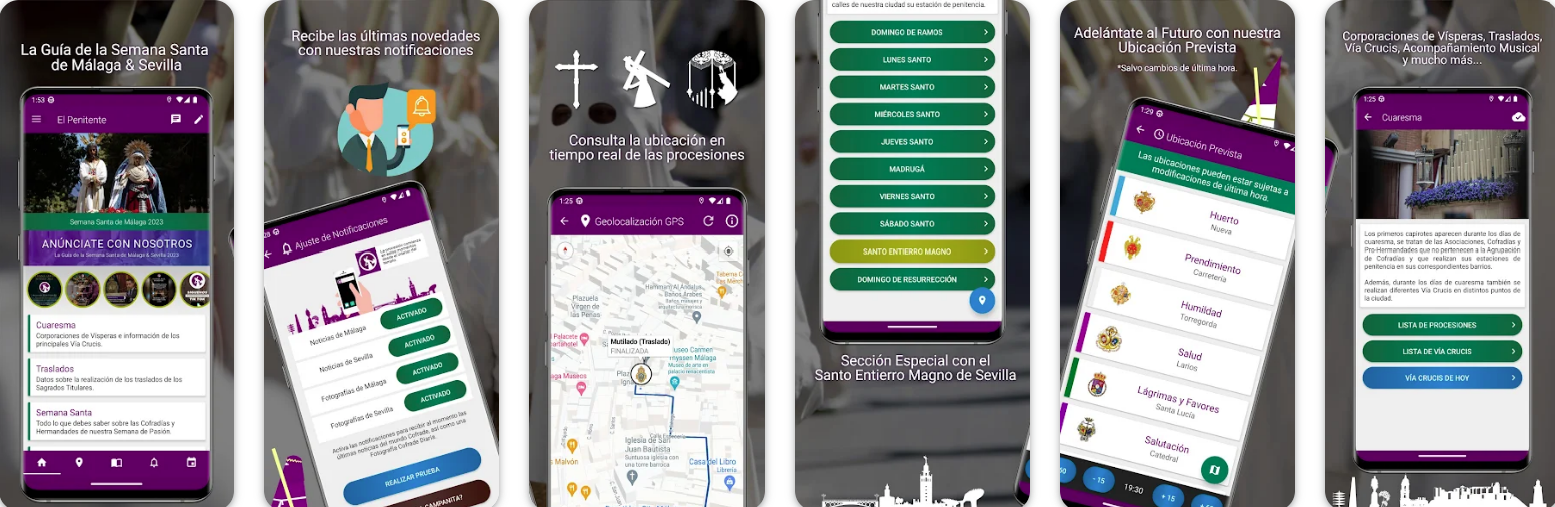
\includegraphics[width=0.9\textwidth]{imagenes/el_penitente.png}
\caption{Interfaz de la aplicación El Penitente \cite{fotosElpenitente}}
\label{fig:penitente}
\end{figure}

Su mayor limitación es que está diseñada y pensada para ciudades específicas y no constituye una solución unificada a nivel nacional.

Otra aplicación a analizar es \textit{Valladolid Cofrade} \cite{valladolidCofrade}, una herramienta reciente desarrollada como aplicación web progresiva (PWA) \cite{queEsPWA}, es decir, una aplicación accesible desde el navegador que puede instalarse en el dispositivo y funcionar de forma similar a una aplicación nativa. Esta permite a los usuarios acceder a información sobre la Semana Santa sin realizar la instalación tradicional desde tiendas oficiales. La aplicación ofrece información sobre programas, recorridos y un sistema de avisos y notificaciones en tiempo real ante cambios o incidencias (Figura \ref{fig:valladolid_cofrade}).

\begin{figure}[ht!]
\centering
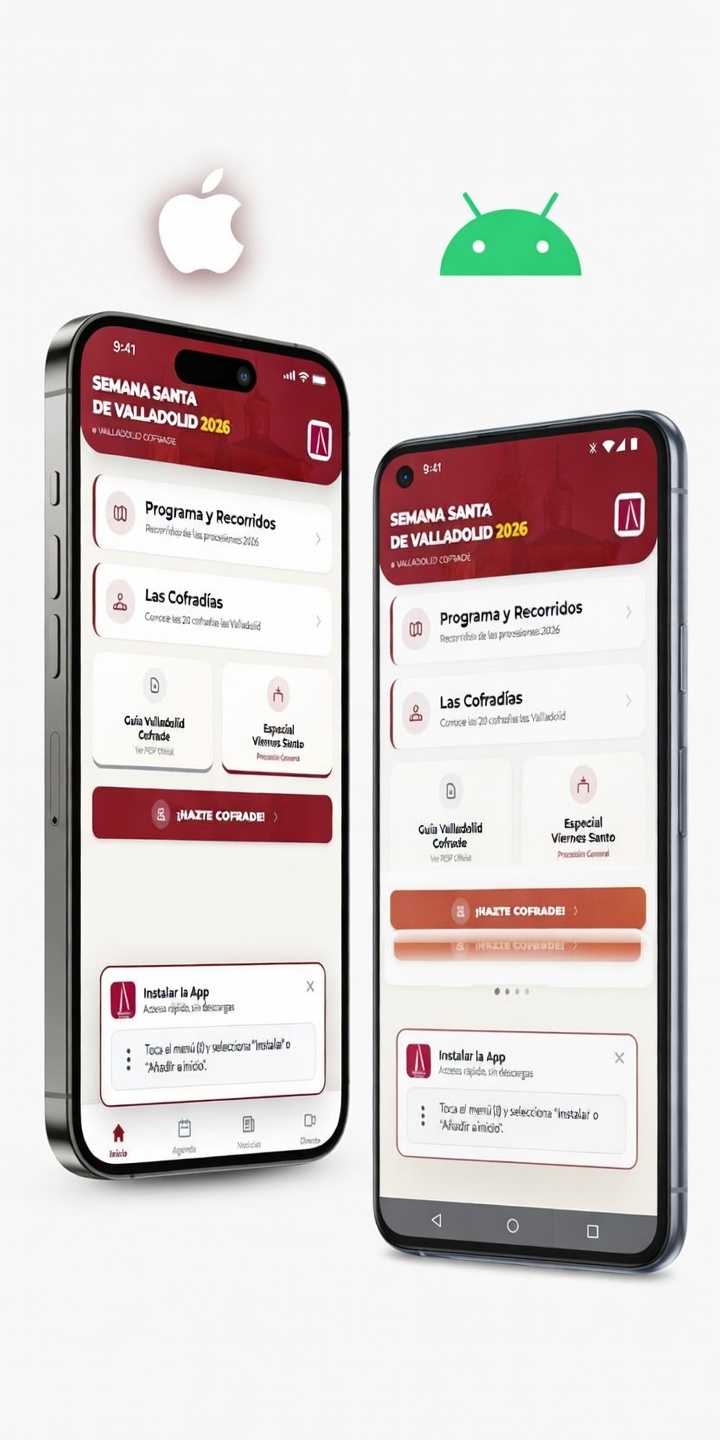
\includegraphics[width=0.4\textwidth]{imagenes/valladolid_cofrade.jpg}
\caption{Interfaz de la aplicación Valladolid Cofrade \cite{valladolidCofrade}}
\label{fig:valladolid_cofrade}
\end{figure}

En otras ciudades se cuenta con aplicaciones locales específicas o sitios web adaptados, como sSantaZgz en Zaragoza \cite{sSantaZgz} o Junta Pro Semana Santa de Zamora \cite{juntaZamora}. Estas aplicaciones muestran el programa oficial, los distintos recorridos e incluso, en algunos casos, como en la de Zamora, incluyen herramientas para conocer la previsión meteorológica.

Más allá de estas limitaciones técnicas, también hay que destacar la diversidad organizativa de la Semana Santa en España, ya que esta depende de la ciudad, de la estructura que se siga en ella y de la terminología utilizada. Por ejemplo, en algunas ciudades, como Valladolid, es común emplear los términos \textit{cofradía} o \textit{cofrade}, mientras que en otras, como Sevilla, se utilizan \textit{hermandad} o \textit{nazareno} para referirse a conceptos equivalentes. Desde el punto de vista organizativo, existen diferentes formas de organizar los eventos, recorridos e itinerarios de las procesiones. Incluso hay diferencias en elementos como pasos, imágenes, homilías, rezos o cánticos que forman parte de estas procesiones o eventos.

Estas diferencias hacen que cada aplicación tenga un diseño distinto, pensado específicamente para una ciudad concreta, dificultando la creación de una solución reutilizable. Por tanto, en la actualidad no existe una plataforma que consiga unificar y generalizar estos conceptos y ofrecer una visión global de la Semana Santa.

Además de las aplicaciones, los usuarios también hacen uso de las publicaciones oficiales de las cofradías en sus páginas web o de programas impresos. Sin embargo, los medios que realmente resultan útiles para la actualización inmediata de la información son las redes sociales oficiales de las cofradías o de las Juntas de Cofradías, que permiten a los espectadores recibir información sobre cambios o comunicados al instante. Aun así, esta forma de comunicación no siempre resulta fácil de encontrar o de organizar debido a la diversidad de cuentas que gestionan dicha información.

\subsection{Aplicaciones de seguimiento en tiempo real}

En cuanto a la geolocalización y el seguimiento en tiempo real, se trata de una tecnología ya existente que se utiliza en diversas aplicaciones como \textit{Google Maps} \cite{googlemapsapi}, que permite conocer la ubicación, cómo llegar a distintos destinos o el estado del transporte público (Figura \ref{fig:googlemaps}).

\begin{figure}[ht!]
\centering
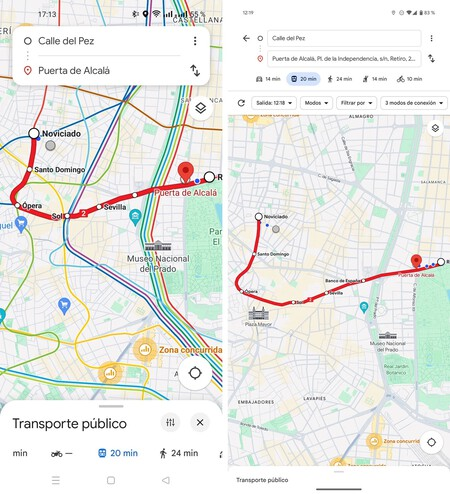
\includegraphics[width=0.6\textwidth]{imagenes/googlemaps.jpeg}
\caption{Ejemplo de geolocalización en tiempo real en Google Maps}
\label{fig:googlemaps}
\end{figure}

Además, plataformas como \textit{Uber} \cite{uber} permiten a los usuarios conocer en todo momento la ubicación exacta del vehículo solicitado (Figura \ref{fig:uber}).

\begin{figure}[ht!]
\centering
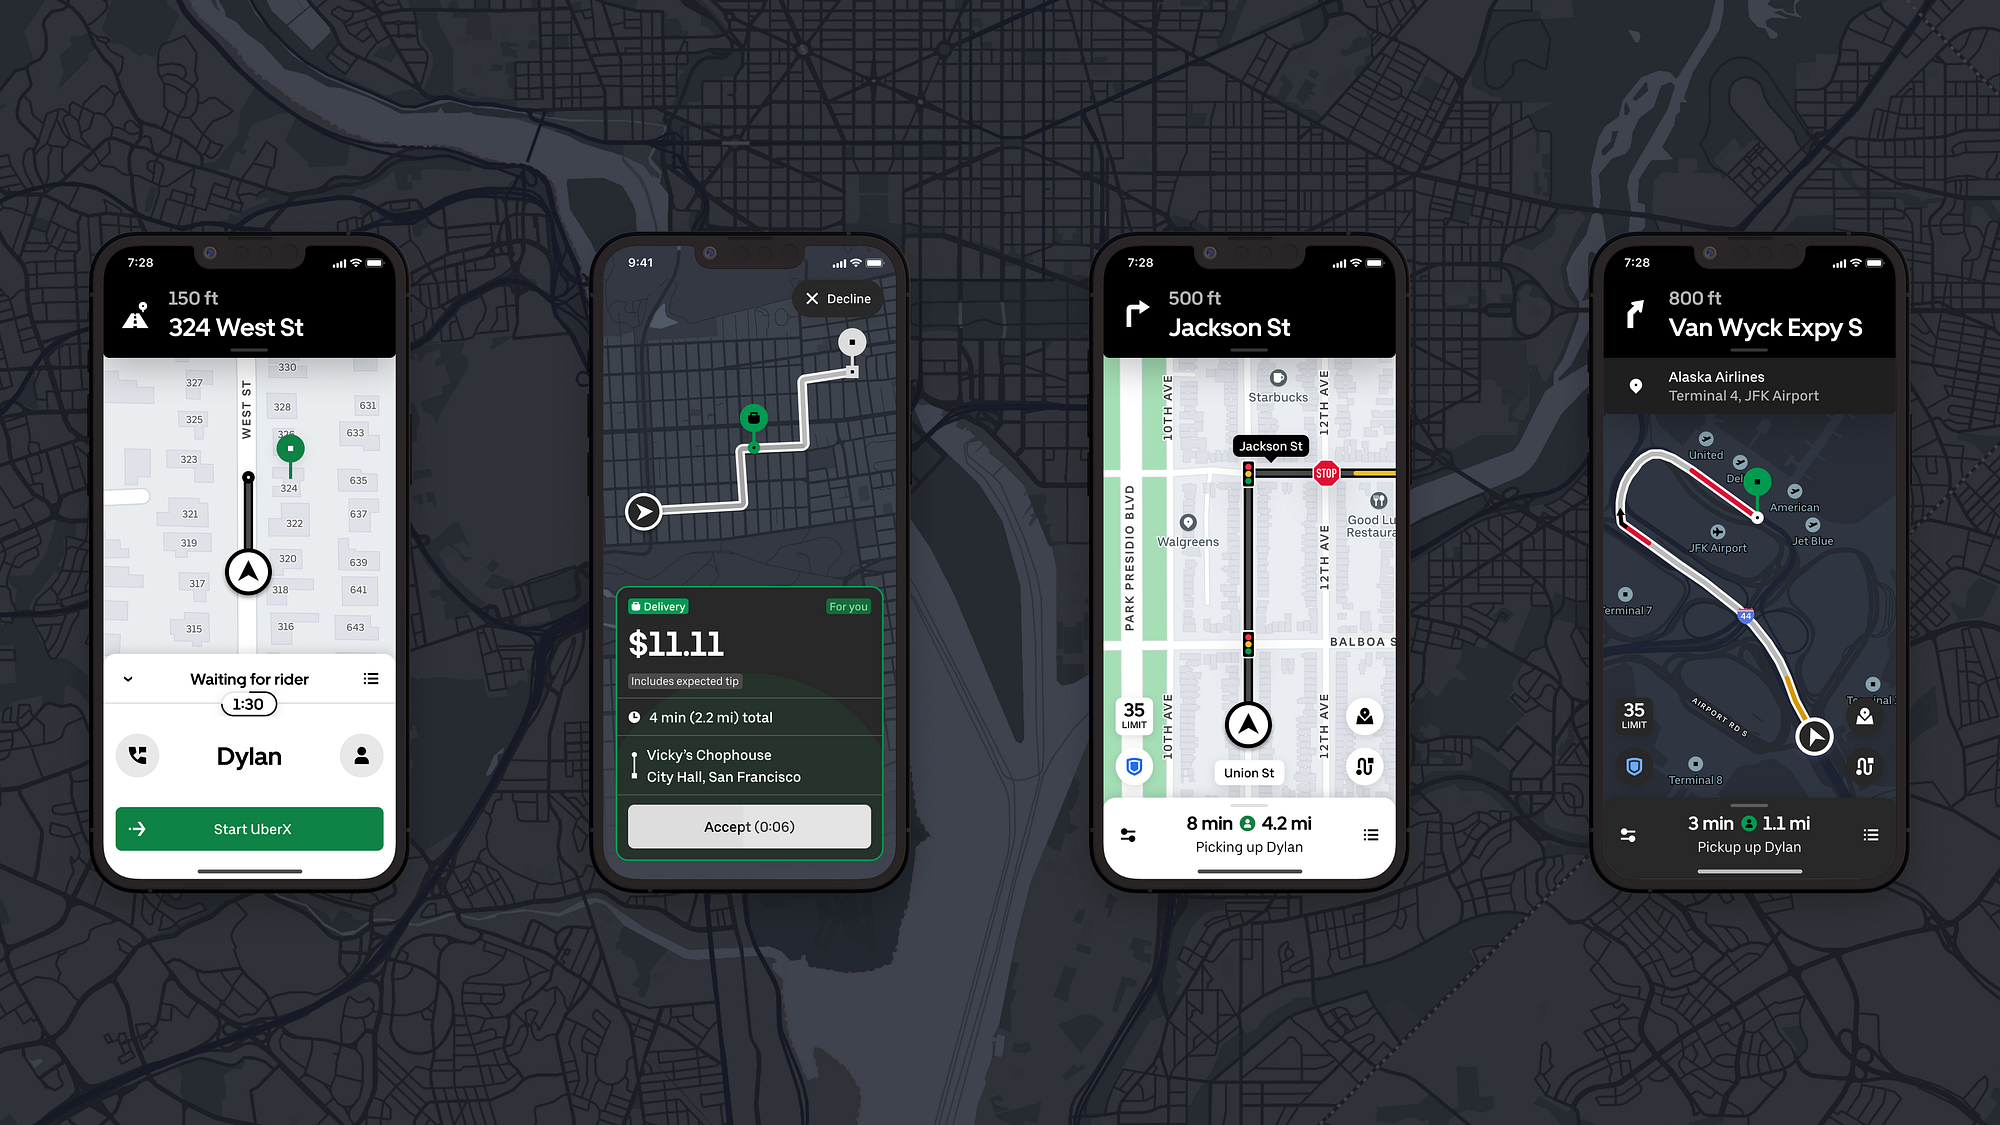
\includegraphics[width=0.8\textwidth]{imagenes/uber.png}
\caption{Seguimiento en tiempo real de un vehículo en Uber}
\label{fig:uber}
\end{figure}

Además, existen diversos Trabajos de Fin de Grado centrados en el desarrollo de aplicaciones móviles y el uso de tecnologías de geolocalización. Un ejemplo es el proyecto realizado por Mario Llorente Pérez \cite{marioTFG}, enfocado en una aplicación móvil relacionada con actividades deportivas y el uso de mapas y geolocalización. En trabajos como este puede observarse el importante papel que juega la localización en tiempo real y la necesidad de diseñar interfaces que permitan al usuario interactuar con la aplicación de forma sencilla.

Todas estas aplicaciones y trabajos constituyen ejemplos claros de que el seguimiento en tiempo real es una funcionalidad ampliamente utilizada, a pesar de que en el contexto de la Semana Santa sigue estando limitada y, cuando se ofrece, suele restringirse a entornos locales o presentar un nivel de precisión reducido.

Por tanto, su incorporación en una solución a nivel nacional conseguiría no solo mejorar la experiencia de los usuarios, sino también superar las limitaciones de las soluciones actuales en cuanto a la oferta de información precisa sobre el estado y la ubicación de las procesiones o eventos.

\section{Objetivos}\label{cap:objetivos}

El objetivo principal de este Trabajo de Fin de Grado es el diseño y desarrollo de una aplicación móvil orientada a la Semana Santa, capaz de centralizar en una única plataforma la información de las distintas celebraciones de Semana Santa a nivel nacional, con independencia de la ciudad, cofradía o terminología empleada en cada una de ellas. En concreto, se busca ofrecer a los usuarios una herramienta que les permita consultar la información relevante de la Semana Santa de una ciudad y visualizar en tiempo real, mediante geolocalización, la ubicación, el recorrido y el estado de sus procesiones.

Para alcanzar este objetivo, se plantean los siguientes objetivos específicos:

\begin{itemize}
\item Diseñar dicha aplicación permitiendo a los usuarios elegir entre las distintas Semanas Santas dentro del territorio nacional.
\item Proporcionar acceso a la información general relacionada con la Semana Santa, incluyendo historia, cofradías o hermandades y elementos representativos.
\item Mostrar información detallada sobre los eventos, como nombre, descripción, fechas, horas e itinerarios.
\item Añadir funcionalidades de personalización, como la selección de eventos o elementos de interés y la recepción de notificaciones ante cambios o incidencias.
\item Implementar un sistema de visualización sobre mapa que permita representar las procesiones y su evolución en tiempo real.
\item Facilitar la navegación del usuario mediante la posibilidad de calcular rutas hacia ubicaciones concretas relacionadas con los eventos.
\item Desarrollar una solución accesible desde dispositivos móviles que garantice una experiencia de uso adecuada.
\item Diseñar una arquitectura escalable que permita la incorporación de nuevas ciudades y eventos sin necesidad de rediseñar el sistema.
\end{itemize}

\section{Estructura de la memoria}\label{cap:estructura_memoria}

Se debe actualizar al terminar el TFG!!!!!!!!!!!!!!!!!!!!!


La memoria se ha organizado en distintos capítulos en los cuales se puede ver la estructura y el desarrollo de dicho proyecto, de forma que se pueda comprender el proyecto de forma clara y completa.

En primer lugar, en este capítulo de introducción se presenta el contexto del proyecto, la motivación que lo impulsa, el estado actual de las distintas soluciones existentes, así como los objetivos que se llevan a cabo.

Después, en el capítulo de planificación se describe la metodología seguida durante el desarrollo de la aplicación, la organización del proyecto, además de las distintas fases de desarrollo y gestión de tareas.

A continuación, en el capítulo de análisis se identifican los actores del sistema, se especifican los requisitos funcionales, de información y no funcionales, y se detallan los casos de uso y el modelo de dominio sobre los que se sustenta el desarrollo de la aplicación.

Seguido por el capítulo de las iteraciones, en el cual se muestran las distintas etapas en las que se ha dividido y repartido el desarrollo de la aplicación, mostrando la evolución que ha ido teniendo el sistema a lo largo del desarrollo del proyecto.

Además, cuenta con un capítulo de estado, en el que se muestra el estado final del sistema desarrollado.

Por último, incluye un capítulo de pruebas en el que se analizan los resultados obtenidos al conseguir construir la versión final y operativa de la aplicación.

Esta memoria concluye con un capítulo de conclusiones, donde se valoran los objetivos conseguidos y se plantean posibles mejoras futuras.
%

\chapter{Planificación}\label{cap:planificacion}
\section{Metodología}\label{cap:metodología}

Para el desarrollo de este proyecto se ha decidido hacer uso de una metodología \textbf{iterativa incremental} \cite{sommerville2015}. Este modelo se ha seleccionado porque permite organizar el proyecto en ciclos o iteraciones sucesivas, donde cada una añade funcionalidad al sistema de forma progresiva. Cada iteración incluye sus propias fases de análisis, diseño, implementación y pruebas, lo que facilita la validación continua del producto y la detección temprana de errores.

La elección de esta metodología está justificada por la naturaleza del proyecto, ya que permite entregar incrementos funcionales del sistema de manera gradual, comenzando por las funcionalidades básicas del módulo ciudadano y avanzando progresivamente hacia características más complejas como la geolocalización en tiempo real, los paneles de gestión y el sistema de notificaciones. Al ser un proyecto desarrollado por un único desarrollador, este modelo resulta adecuado porque combina la flexibilidad de adaptarse a posibles ajustes durante el desarrollo con una planificación estructurada que facilita el seguimiento del avance.

El proyecto se ha organizado en una \textbf{fase inicial de análisis} general, seguida de \textbf{cinco iteraciones} que abordan de forma incremental los distintos módulos del sistema, y una \textbf{fase final} de documentación, integración y entrega.
\section{Planificación, Fases e iteraciones}\label{cap:planificacionExtensa}

\subsection{Planificación inicial}

Este proyecto consta de tres grandes fases, cuya planificación general se puede observar en el siguiente Diagrama de Gantt \cite{diagramaGantt} (Figura \ref{fig:DiagramaGanttCompleto}): una primera fase de análisis, una segunda fase de desarrollo iterativo e incremental, organizada en cinco iteraciones, y una tercera y última fase de documentación y entrega.

\begin{figure}[H]
    \centering
    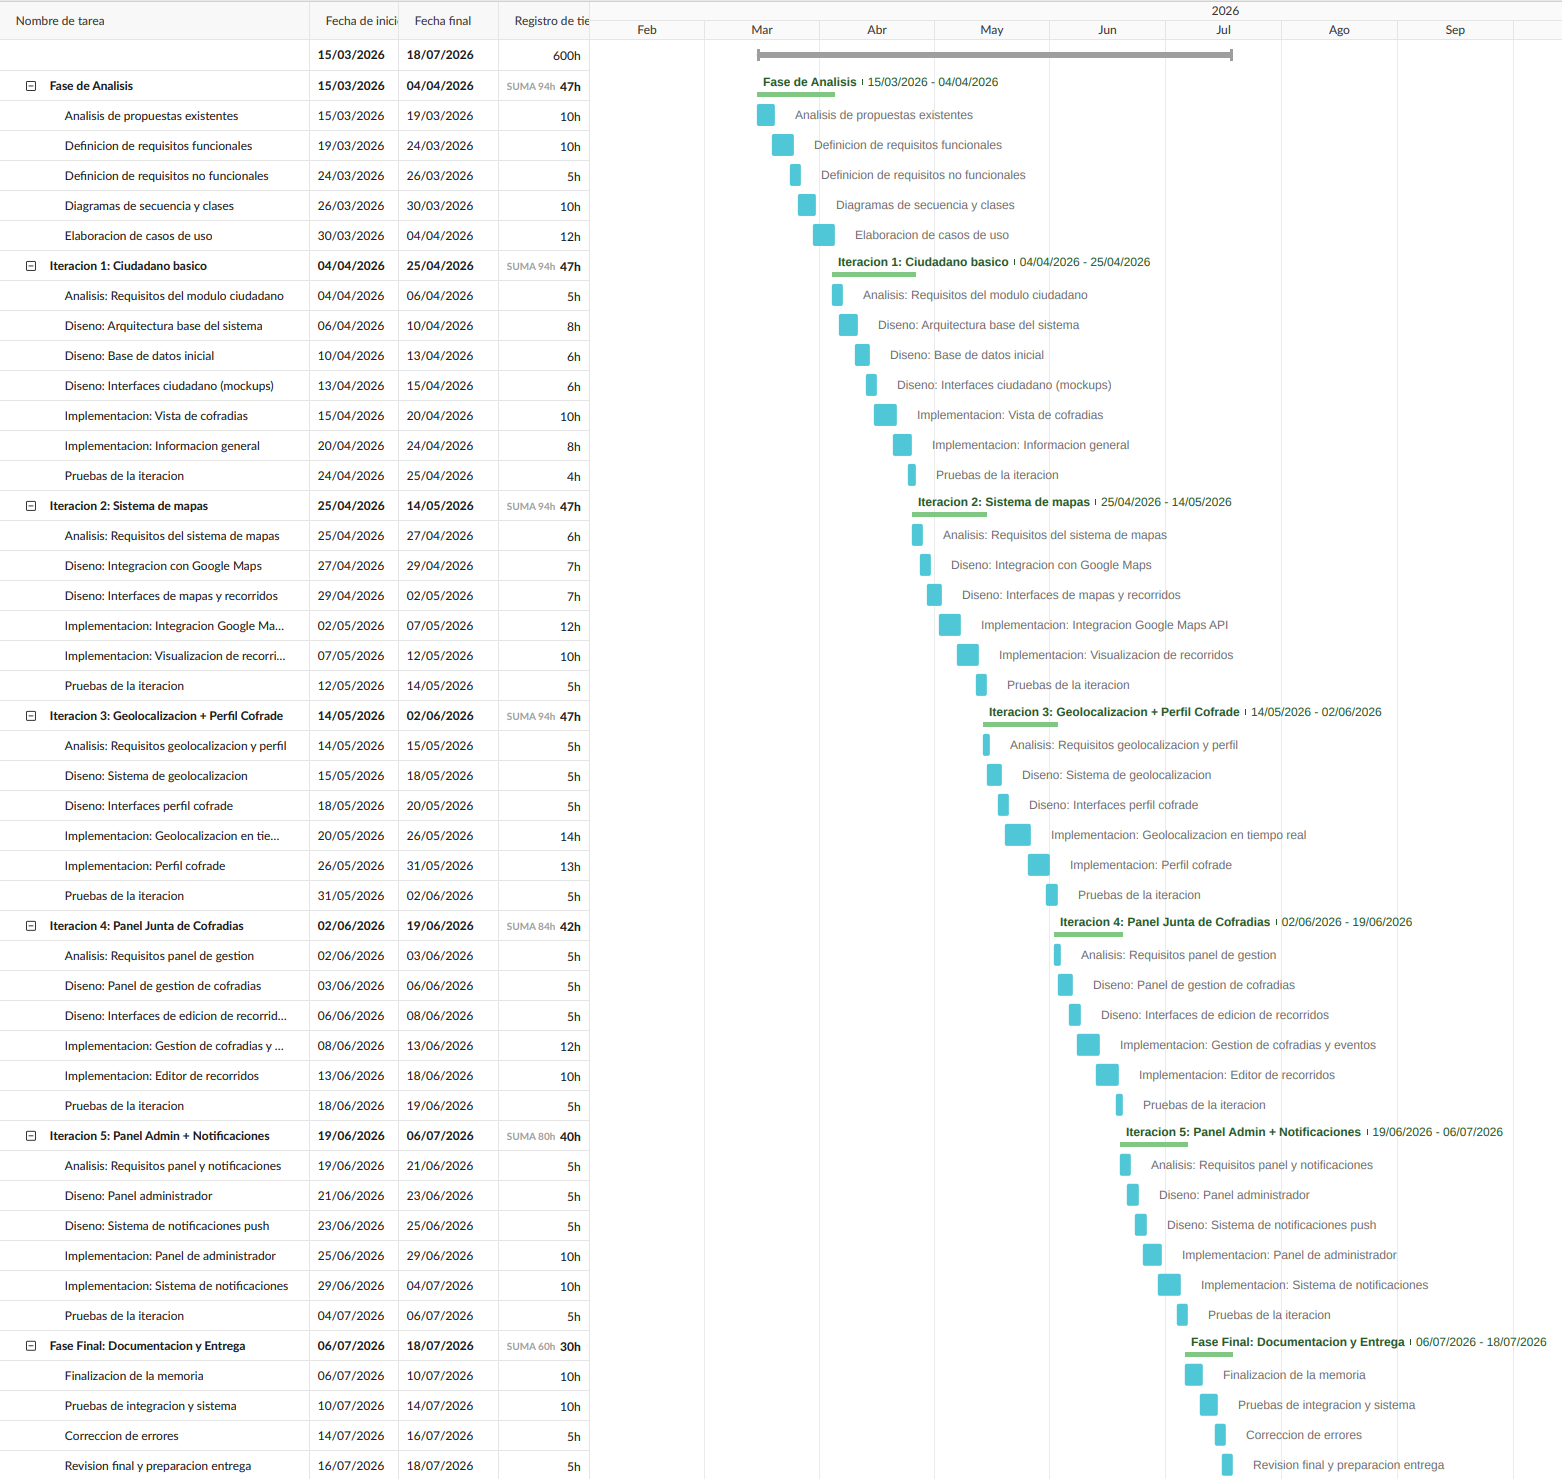
\includegraphics[width=1\textwidth]{imagenes/DiagramaGantBig.png}
    \caption{Diagrama de Gantt general completo del proyecto}
    \label{fig:DiagramaGanttCompleto}
\end{figure}

\subsection{Fase de análisis}

Esta primera fase se centra en el análisis de las aplicaciones relacionadas con la Semana Santa existentes, la identificación de sus carencias y áreas de mejora, y en la definición extendida de los requisitos funcionales y no funcionales \cite{ieee29148} del sistema, además de la elaboración de los casos de uso \cite{uml} y los distintos diagramas que servirán como base para la realización del desarrollo de la aplicación.

Esta fase comienza con el análisis de las propuestas existentes en el mercado, identificando las características principales de aplicaciones como \textit{El Penitente} \cite{elpenitente}, \textit{Valladolid Cofrade} \cite{valladolidCofrade} o \textit{sSantaZgz} \cite{sSantaZgz}.

Seguido de este análisis se realiza la definición de los requisitos funcionales, los cuales describen las funcionalidades concretas que el sistema debe ofrecer, y los requisitos no funcionales, que definen las condiciones de calidad, rendimiento y seguridad que debe cumplir \cite{ieee29148}, teniendo en cuenta los cuatro perfiles de usuario: ciudadano, cofrade, Junta de Cofradías y administrador. También se elaboran los diagramas de secuencia y el modelo de dominio, así como los casos de uso \cite{uml}, representaciones estandarizadas de las interacciones entre los usuarios y el sistema, que servirán para el desarrollo posterior.

\subsection{Fase de iteraciones}

Esta segunda fase está centrada en el diseño e implementación de la aplicación de forma iterativa e incremental \cite{larman2004}. Aunque el marco general del proyecto sigue el modelo en cascada --en el sentido de que el análisis es seguido del diseño y tras este la implementación--, en esta fase se aplica un ciclo interno de análisis, diseño, implementación y pruebas en cada iteración, lo que permite ir incorporando las funcionalidades de forma progresiva y verificando su correcto funcionamiento antes de darla por finalizada y avanzar a la siguiente. El desglose detallado de tareas y horas de cada iteración puede consultarse en el Diagrama de Gantt (Figura~\ref{fig:DiagramaGanttCompleto}).

Estas iteraciones abarcan desde las funcionalidades básicas del ciudadano hasta las más complejas, como la geolocalización en tiempo real, es decir, la capacidad de conocer y actualizar la posición geográfica de una procesión de forma continua haciendo uso de la tecnología GPS\footnote{GPS (Global Positioning System): sistema de navegación por satélite que permite determinar la posición geográfica de un dispositivo en cualquier punto del planeta.} del móvil, o el sistema de notificaciones (mensajes enviados desde el servidor a los dispositivos de los usuarios sin que estos tengan que abrir la aplicación activamente).

\subsubsection{Iteración 1: Módulo ciudadano básico}

Esta primera iteración tiene como objetivo establecer la arquitectura base del sistema y desarrollar las funcionalidades fundamentales del perfil de ciudadano, entre las que se incluyen la visualización de la información general de la Semana Santa, el listado de organizaciones y la consulta de eventos.

\subsubsection{Iteración 2: Sistema de mapas}

Esta segunda iteración se centra principalmente en la implementación del sistema de mapas, que permitirá visualizar los distintos recorridos de las procesiones.

\subsubsection{Iteración 3: Geolocalización y perfil cofrade}

Esta tercera iteración se centra en la implementación completa del sistema de geolocalización en tiempo real, de forma que se pueda conocer y actualizar de manera continua la posición de las procesiones durante su recorrido. Además, se desarrolla el perfil de cofrade con sus correspondientes funcionalidades, incluyendo la posibilidad de compartir la ubicación durante las procesiones.

\subsubsection{Iteración 4: Panel de la Junta de Cofradías}

Esta cuarta iteración corresponde al desarrollo del panel de gestión para las Juntas de Cofradías, permitiendo administrar la información de la Semana Santa, incluyendo eventos, recorridos, imágenes y participantes. El acceso a este panel está restringido mediante un mecanismo de control de acceso \cite{owasp}, que permite diferenciar los permisos y limitaciones de los distintos roles del sistema.

\subsubsection{Iteración 5: Panel de administrador y notificaciones}

Esta quinta y última iteración se centra en la implementación del panel de administrador global del sistema, así como del sistema de notificaciones, que permitirá a la Junta de Cofradías comunicar a los usuarios cambios o incidencias en las procesiones de forma inmediata, sin necesidad de que estos tengan la aplicación abierta.

\subsection{Fase final: documentación y entrega}

En esta última fase se realizan las pruebas de integración del sistema completo, la corrección de errores detectados, la finalización de la memoria del proyecto y la preparación de la entrega final.

\section{Análisis de riesgos}\label{cap:analisisRiesgos}

Otra parte importante en la planificación de un proyecto de desarrollo de software es el análisis de riesgos. Un riesgo es un evento de incertidumbre que puede afectar de forma positiva o negativa a los objetivos del proyecto \cite{pmbok}. Para garantizar el alcance de los objetivos del proyecto, es necesario realizar un análisis de estos riesgos.

Los riesgos identificados se organizan en función de su prioridad, la cual se determina mediante la técnica de análisis de exposición al riesgo (\textit{Risk Exposure}, RE) \cite{boehm}, donde el riesgo se calcula mediante un valor numérico que representa la probabilidad e impacto estimados de cada evento. Se define de la siguiente manera:

\begin{equation}
    RE = \text{probabilidad} \times \text{impacto}
\end{equation}

La variable probabilidad representa la probabilidad de que el riesgo se materialice en el proyecto (escala de 1 a 10), mientras que el impacto representa la gravedad de sus consecuencias en caso de ocurrir (escala de 1 a 10). En la Tabla~\ref{tab:riesgos} se muestran los riesgos identificados en el proyecto.

\begin{table}[ht!]
\centering
\begin{tabular}{|l|c|c|c|}
\hline
\textbf{Riesgo} & \textbf{Probabilidad} & \textbf{Impacto} & \textbf{Prioridad} \\
\hline
1. Estimaciones de tiempo erróneas & 8 & 7 & 56 \\
\hline
2. Problemas con la integración de Google Maps & 6 & 8 & 48 \\
\hline
3. Errores durante el desarrollo & 7 & 6 & 42 \\
\hline
4. Falta de experiencia con tecnologías móviles & 7 & 6 & 42 \\
\hline
5. Problemas con la geolocalización en tiempo real & 5 & 8 & 40 \\
\hline
6. Cambios en los requisitos & 6 & 6 & 36 \\
\hline
7. Especificaciones ambiguas o poco definidas & 5 & 6 & 30 \\
\hline
8. Problemas con el entorno de desarrollo & 4 & 5 & 20 \\
\hline
9. Indisponibilidad del desarrollador & 3 & 6 & 18 \\
\hline
10. Problemas con Firebase o la base de datos & 3 & 5 & 15 \\
\hline
\end{tabular}
\caption{Riesgos identificados en el proyecto}
\label{tab:riesgos}
\end{table}

\subsection{Planificación de riesgo}

Tras realizar la identificación de los riesgos, el siguiente paso es la decisión de qué medidas se deben tomar para reducir la probabilidad de que el riesgo ocurra, de forma que se pueda disminuir su impacto una vez se materialice.

\begin{table}[ht!]
\centering
\begin{tabular}{|p{3cm}|p{10cm}|}
\hline
\textbf{Riesgo} & Estimaciones de tiempo erróneas \\
\hline
\textbf{Reducción} & Planificar las tareas con margen por si la estimación ha sido inferior al tiempo necesario. Dividir las tareas grandes en subtareas más pequeñas y manejables. \\
\hline
\textbf{Contingencia} & Cambiar la planificación, reducir el alcance del proyecto priorizando las funcionalidades esenciales. \\
\hline
\end{tabular}
\caption{Riesgo 1: Estimaciones de tiempo erróneas}
\end{table}

\begin{table}[ht!]
\centering
\begin{tabular}{|p{3cm}|p{10cm}|}
\hline
\textbf{Riesgo} & Problemas con la integración de Google Maps \\
\hline
\textbf{Reducción} & Realizar pruebas de concepto tempranas con la API de Google Maps. Documentarse sobre las limitaciones y cuotas del servicio. \\
\hline
\textbf{Contingencia} & Considerar alternativas como OpenStreetMap \cite{openstreetmap} o Mapbox en caso de problemas persistentes. \\
\hline
\end{tabular}
\caption{Riesgo 2: Problemas con la integración de Google Maps}
\end{table}

\begin{table}[ht!]
\centering
\begin{tabular}{|p{3cm}|p{10cm}|}
\hline
\textbf{Riesgo} & Errores durante el desarrollo \\
\hline
\textbf{Reducción} & Verificar que la funcionalidad está implementada correctamente antes de dar por finalizado el incremento. Realizar pruebas unitarias\footnote{Pruebas unitarias: pruebas que verifican el correcto funcionamiento de componentes individuales del código de forma aislada.}. \\
\hline
\textbf{Contingencia} & Volver al último punto correctamente probado y continuar desde ahí. Utilizar control de versiones \cite{github} para recuperar estados anteriores del código. \\
\hline
\end{tabular}
\caption{Riesgo 3: Errores durante el desarrollo}
\end{table}

\begin{table}[ht!]
\centering
\begin{tabular}{|p{3cm}|p{10cm}|}
\hline
\textbf{Riesgo} & Falta de experiencia con tecnologías móviles \\
\hline
\textbf{Reducción} & Formarse en las tecnologías clave antes de proceder al desarrollo. Consultar documentación oficial y tutoriales. \\
\hline
\textbf{Contingencia} & Aprovechar la experiencia del tutor para solventar los posibles problemas. Buscar soluciones en comunidades de desarrolladores. \\
\hline
\end{tabular}
\caption{Riesgo 4: Falta de experiencia con tecnologías móviles}
\end{table}

\begin{table}[ht!]
\centering
\begin{tabular}{|p{3cm}|p{10cm}|}
\hline
\textbf{Riesgo} & Problemas con la geolocalización en tiempo real \\
\hline
\textbf{Reducción} & Investigar las mejores prácticas para implementar geolocalización en aplicaciones móviles. Realizar prototipos tempranos para validar la viabilidad técnica. \\
\hline
\textbf{Contingencia} & Implementar un modo de actualización manual de la ubicación como alternativa temporal. \\
\hline
\end{tabular}
\caption{Riesgo 5: Problemas con la geolocalización en tiempo real}
\end{table}

\begin{table}[ht!]
\centering
\begin{tabular}{|p{3cm}|p{10cm}|}
\hline
\textbf{Riesgo} & Cambios en los requisitos \\
\hline
\textbf{Reducción} & El desarrollo iterativo permite adaptar el sistema a cambios de forma gradual. \\
\hline
\textbf{Contingencia} & Reevaluar las prioridades y ajustar el alcance del proyecto según las nuevas necesidades. \\
\hline
\end{tabular}
\caption{Riesgo 6: Cambios en los requisitos}
\end{table}

\begin{table}[ht!]
\centering
\begin{tabular}{|p{3cm}|p{10cm}|}
\hline
\textbf{Riesgo} & Especificaciones genéricas \\
\hline
\textbf{Reducción} & Reunir toda la información posible antes de abordar una tarea. Clarificar requisitos con el tutor. \\
\hline
\textbf{Contingencia} & Prototipar en caso de ser necesario para validar la interpretación de los requisitos. \\
\hline
\end{tabular}
\caption{Riesgo 7: Especificaciones genéricas}
\end{table}

\begin{table}[ht!]
\centering
\begin{tabular}{|p{3cm}|p{10cm}|}
\hline
\textbf{Riesgo} & Problemas con el entorno de desarrollo \\
\hline
\textbf{Reducción} & Utilizar un repositorio remoto (GitHub \cite{github}) para almacenar copias de seguridad del código. \\
\hline
\textbf{Contingencia} & Utilizar una máquina de respaldo o entorno de desarrollo alternativo. \\
\hline
\end{tabular}
\caption{Riesgo 8: Problemas con el entorno de desarrollo}
\end{table}

\begin{table}[ht!]
\centering
\begin{tabular}{|p{3cm}|p{10cm}|}
\hline
\textbf{Riesgo} & Indisposición del desarrollador \\
\hline
\textbf{Reducción} & Planificar las tareas con margen por si es necesario extender el tiempo para completar el incremento. \\
\hline
\textbf{Contingencia} & Realizar horas extra en caso necesario y ajustar la planificación. \\
\hline
\end{tabular}
\caption{Riesgo 9: Indisposición del desarrollador}
\end{table}

\begin{table}[ht!]
\centering
\begin{tabular}{|p{3cm}|p{10cm}|}
\hline
\textbf{Riesgo} & Problemas con Firebase/base de datos \\
\hline
\textbf{Reducción} & Documentarse sobre las limitaciones del plan gratuito de Firebase \cite{firebasefcm}. Diseñar una estructura de datos eficiente. \\
\hline
\textbf{Contingencia} & Migrar a un servicio alternativo en caso de problemas críticos. \\
\hline
\end{tabular}
\caption{Riesgo 10: Problemas con Firebase/base de datos}
\end{table}

\subsection{Monitorización de riesgos}

Durante el desarrollo del proyecto, se debe realizar un seguimiento continuo de los riesgos identificados para detectar de forma temprana su aparición y poder aplicar las medidas pertinentes.

\textit{!!!!!!!!!!!!!!!!!!!!!!!!!!!!!!Nota : Esta sección se completará al finalizar el desarrollo del proyecto, documentando qué riesgos se manifestaron, el impacto que tuvieron y las medidas que se tomaron para subsanarlos.}

\section{Seguimiento del proyecto}\label{cap:planificacionFinal}

\textit{Nota: Esta sección se completará al finalizar el desarrollo del proyecto, comparando la planificación inicial con la duración real del proyecto.}
comentar que ha habido distintas planificacion debedo a diversos cortatimepo que han surguido a lo largo de los mese de desarrollo
% Se incluirá un diagrama de Gantt con la duración real del proyecto:
% \begin{figure}[H]
%     \centering
%     \includegraphics[width=1\textwidth]{imagenes/GanttReal.pdf}
%     \caption{Diagrama de Gantt de la duración real del proyecto}
%     \label{fig:GanttReal}
% \end{figure}

\subsection{Monitorización de riesgos}

Durante el desarrollo del proyecto, se debe realizar un seguimiento continuo de los riesgos identificados para detectar de forma temprana su aparición y poder aplicar las medidas pertinentes.

\textit{!!!!!!!!!!!!!!!!!!!!!!!!!!!!!!Nota : Esta sección se completará al finalizar el desarrollo del proyecto, documentando qué riesgos se manifestaron, el impacto que tuvieron y las medidas que se tomaron para subsanarlos.}

\section{Estimación de costes}\label{cap:estimacionCostes}

A continuación se presenta el presupuesto estimado del proyecto, calculado como si este fuese desarrollado por un equipo profesional completo, siguiendo los perfiles habituales en el desarrollo de una aplicación móvil de estas características. Se trata de una estimación teórica con fines de planificación y no de los costes reales asumidos por el autor, quien ha desarrollado el TFG de forma individual.

\subsection{Costes de personal}

Un proyecto de estas características, correspondiente al desarrollo completo de una aplicación móvil sobre la Semana Santa, requeriría en un entorno profesional un equipo multidisciplinar. Se han considerado los siguientes seis perfiles, entre los que se reparten las 300 horas estimadas de duración del proyecto:

\begin{itemize}
    \item \textbf{Jefe de Proyecto}: coordinación general, planificación y seguimiento.
    \item \textbf{Analista Funcional}: recogida y especificación de requisitos, análisis del dominio.
    \item \textbf{Diseñador UX/UI}: diseño de la experiencia e interfaz de usuario.
    \item \textbf{Desarrollador Backend}: implementación del servidor, base de datos y API.
    \item \textbf{Desarrollador Frontend/Mobile}: implementación de la aplicación Android.
    \item \textbf{Tester/QA}: pruebas funcionales, de regresión y control de calidad.
\end{itemize}

Para cada perfil se ha calculado el coste por hora a partir del sueldo bruto anual medio en España, incrementado en un 30\% en concepto de cotizaciones a la Seguridad Social a cargo de la empresa, y dividido entre 1.800 horas anuales de jornada completa. La Tabla~\ref{tab:horas_personal} recoge el reparto de horas y el coste asociado a cada perfil.

\begin{table}[ht!]
\centering
\begin{tabular}{|l|r|r|r|}
\hline
\textbf{Perfil} & \textbf{Horas} & \textbf{Coste/hora} & \textbf{Coste total} \\
\hline
Jefe de Proyecto \cite{salarioJefeProyecto}          & 45  & 33€ & 1.485,00€ \\
\hline
Analista Funcional \cite{salarioAnalista}            & 45  & 27€ & 1.215,00€ \\
\hline
Diseñador UX/UI \cite{salarioUXUI}                   & 30  & 27€ &   810,00€ \\
\hline
Desarrollador Backend \cite{salarioBackend}          & 75  & 26€ & 1.950,00€ \\
\hline
Desarrollador Frontend/Mobile \cite{salarios}        & 75  & 19€ & 1.425,00€ \\
\hline
Tester/QA \cite{salarioTester}                       & 30  & 17€ &   510,00€ \\
\hline
\textbf{Total} & \textbf{300} & & \textbf{7.395,00€} \\
\hline
\end{tabular}
\caption{Reparto de horas y coste de personal por perfil}
\label{tab:horas_personal}
\end{table}

\subsection{Costes de equipo y amortización}

El equipo del proyecto necesitaría un ordenador portátil por persona, además de un dispositivo Android dedicado a las pruebas. Se considera una duración total del proyecto de 5 meses.

\begin{itemize}
    \item \textbf{Ordenadores portátiles}: 6 unidades valoradas en 1.000€ cada una, con una vida útil estimada de 5 años (60 meses). La amortización mensual por unidad es de 16,66€, lo que supone 83,30€ por portátil durante los 5 meses del proyecto, y 500,00€ en total para los 6 puestos de trabajo.
    \item \textbf{Dispositivo Android de pruebas}: 1 unidad valorada en 300€, con una vida útil estimada de 3 años (36 meses). La amortización mensual es de 8,33€, lo que supone 41,65€ para los 5 meses del proyecto.
\end{itemize}

Ahora bien, estos importes corresponden a la ocupación de los equipos durante los 5 meses completos del proyecto. Dado que el trabajo real asciende a 300 horas, frente a una capacidad disponible de 750 horas en ese periodo (150 horas/mes de jornada completa, según el criterio de 1.800 horas anuales aplicado en el apartado anterior), el resto del tiempo los equipos podrían destinarse a otro uso. Por ello, la amortización se imputa de forma proporcional al uso real del proyecto (300/750 = 40\%).

El coste de amortización así calculado asciende a \textbf{216,66€}, tal y como recoge la Tabla~\ref{tab:amortizacion}.

\begin{table}[ht!]
\centering
\begin{tabular}{|l|r|r|r|r|}
\hline
\textbf{Recurso} & \textbf{Valor} & \textbf{Vida útil} & \textbf{Amort. (5 meses)} & \textbf{Amort. proporcional (300h, 40\%)} \\
\hline
Portátiles (x6) & 6.000,00€ & 5 años & 500,00€ & 200,00€ \\
\hline
Dispositivo Android (x1) & 300,00€ & 3 años & 41,65€ & 16,66€ \\
\hline
\textbf{Total amortización} & & & 541,65€ & \textbf{216,66€} \\
\hline
\end{tabular}
\caption{Amortización de los recursos de equipo, prorrateada al uso real del proyecto}
\label{tab:amortizacion}
\end{table}

\subsection{Costes de licencias de software}

Buena parte de las herramientas empleadas disponen de planes gratuitos o licencias universitarias suficientes para un proyecto de este tamaño. Sin embargo, un equipo profesional de 6 personas necesitaría además herramientas colaborativas de pago para la gestión del proyecto y el diseño. La Tabla~\ref{tab:licencias} recoge el coste y la fuente de cada licencia.

\begin{table}[ht!]
\centering
\begin{tabular}{|l|r|l|}
\hline
\textbf{Herramienta} & \textbf{Coste} & \textbf{Fuente} \\
\hline
Android Studio & 0,00€ & \cite{androidstudio} \\
\hline
Visual Studio Code & 0,00€ & \cite{vscode} \\
\hline
Overleaf (plan gratuito) & 0,00€ & --- \\
\hline
Google Firebase (plan gratuito) & 0,00€ & \cite{firebasefcm} \\
\hline
Google Maps API (crédito gratuito) & 0,00€ & \cite{googlemapsapi} \\
\hline
GitHub (plan gratuito) & 0,00€ & \cite{github} \\
\hline
Cuenta de desarrollador Google Play (pago único) & 23,00€ & \cite{googlePlayFee} \\
\hline
Figma Professional (1 licencia, 5 meses) & 69,00€ & \cite{figmaPricing} \\
\hline
Jira Software Standard (6 usuarios, 5 meses) & 218,40€ & \cite{jiraPricing} \\
\hline
\textbf{Total licencias} & \textbf{310,40€} & \\
\hline
\end{tabular}
\caption{Coste de licencias de software}
\label{tab:licencias}
\end{table}

\subsection{Otros costes indirectos}

Un equipo de 6 personas trabajando de forma presencial o híbrida necesitaría un espacio de oficina. Se ha tomado como referencia el alquiler de un despacho de 22 m\textsuperscript{2} en un espacio de coworking en el centro de Valladolid, con todos los suministros incluidos (calefacción, refrigeración, electricidad, wifi y limpieza), por un importe de 475€ al mes \cite{oficinaValladolid}. Para los 5 meses de duración del proyecto, el coste estructural asciende a 2.375,00€.

Al igual que con la amortización de equipos, este importe corresponde a la disponibilidad del espacio durante los 5 meses completos, mientras que el uso real del proyecto es de 300 horas frente a una capacidad de 750 horas en ese periodo (40\%); el resto del tiempo el espacio podría destinarse a otro uso. Aplicando este mismo criterio de proporcionalidad, el coste estructural imputado al proyecto asciende a \textbf{950,00€} (2.375,00€ × 40\%).

\subsection{Coste total}

La Tabla~\ref{tab:costes_totales} resume el presupuesto completo del proyecto, considerando personal, amortización de equipo, licencias de software y costes estructurales —estos dos últimos prorrateados a las 300 horas reales de uso— para una duración de 300 horas repartidas en 5 meses.

\begin{table}[ht!]
\centering
\begin{tabular}{|l|r|}
\hline
\textbf{Elemento} & \textbf{Coste} \\
\hline
Personal (Tabla~\ref{tab:horas_personal}) & 7.395,00€ \\
\hline
Amortización de equipo, prorrateada (Tabla~\ref{tab:amortizacion}) & 216,66€ \\
\hline
Licencias de software (Tabla~\ref{tab:licencias}) & 310,40€ \\
\hline
Costes estructurales, prorrateados (oficina y suministros) & 950,00€ \\
\hline
\textbf{Total} & \textbf{8.872,06€} \\
\hline
\end{tabular}
\caption{Costes totales del proyecto}
\label{tab:costes_totales}
\end{table}

\subsection{Coste estimado de Firebase en producción}\label{cap:costeFirebaseProduccion}

Los costes anteriores corresponden únicamente al desarrollo del TFG, durante el cual el uso de Firebase se ha mantenido dentro de la capa gratuita (plan \textit{Spark}). Sin embargo, tal y como se señala en la Sección~\ref{cap:puntosDebiles}, el paso a producción con usuarios reales implicaría migrar al plan de pago \textit{Blaze}, facturado según el consumo real. A modo orientativo, y tomando las tarifas oficiales vigentes del plan Blaze para Cloud Firestore \cite{firebasepricing} --0,06 € por cada 100.000 lecturas, 0,18 € por cada 100.000 escrituras y 0,26 € por GB almacenado al mes, descontando la cuota gratuita diaria de 50.000 lecturas y 20.000 escrituras--, se puede estimar el coste de una semana de Semana Santa en una única ciudad piloto:

\begin{itemize}
    \item \textbf{Lecturas}: suponiendo 3.000 usuarios simultáneos consultando el mapa en tiempo real durante una media de 3 horas al día, con actualizaciones cada 30 segundos (RNF-08), se generarían unas 360 lecturas por usuario y día, es decir, aproximadamente 1.080.000 lecturas diarias (7.560.000 en los 7 días de Semana Santa). Descontando la cuota gratuita, el coste asciende a unos \textbf{4,30 €}.
    \item \textbf{Escrituras}: suponiendo 200 cofrades compartiendo su ubicación durante 2 horas al día (240 escrituras por cofrade y día), se generarían unas 48.000 escrituras diarias (336.000 en los 7 días). Descontando la cuota gratuita, el coste asciende a unos \textbf{0,35 €}.
    \item \textbf{Almacenamiento y notificaciones}: el volumen de datos almacenado (perfiles, códigos de acceso, información de cofradías y procesiones) se mantendría muy por debajo de 1~GB, dentro de la cuota gratuita; Cloud Messaging no tiene coste en el plan Blaze \cite{firebasepricing}.
\end{itemize}

Bajo estas hipótesis, el coste de Firebase para una semana de Semana Santa en una ciudad piloto rondaría los \textbf{5 €}, una cifra reducida gracias al bajo coste unitario de las operaciones de Firestore. No obstante, este importe crecería proporcionalmente al escalar la aplicación a más ciudades y usuarios, tal y como se plantea en el trabajo futuro (Sección~\ref{cap:trabajo_futuro}), por lo que esta estimación --y las hipótesis de partida sobre el número de usuarios y ciudades-- debería revisarse y ajustarse junto con el tutor antes de un despliegue real en producción.

\chapter{Análisis}\label{cap:analisis}
\section{Requisitos}
\label{cap:requisitos}

% Comando para indicar la prioridad de un requisito de forma uniforme.
\newcommand{\prioridad}[1]{\textit{(Prioridad: #1)}}

\subsection{Requisitos funcionales}

Los requisitos funcionales definen las diferentes funciones del sistema, además de cómo debe ser su comportamiento en ciertas situaciones. Cada requisito incluye, junto a su descripción, el nivel de prioridad asignado (Alta, Media o Baja), que indica su importancia relativa dentro del proyecto.

Para facilitar su lectura, los requisitos se han agrupado según el perfil de usuario (Sección~\ref{cap:analisis_usuarios}) al que van dirigidos --ciudadano, cofrade, Junta de Cofradías o administrador--. Dentro de cada grupo se han ordenado de mayor a menor prioridad, salvo en el del ciudadano: al ser el grupo más numeroso, sus requisitos se listan siguiendo en su lugar el flujo de uso habitual de la aplicación (desde que se accede hasta la geolocalización en tiempo real y las notificaciones), para que el lector pueda seguirlos en el mismo orden en que se encontraría con ellos. Además el perfil de cofrade incluye, a mayores de los requisitos propios de dicho perfil, todos los requisitos del ciudadano, ya que un cofrade puede hacer uso de todas las funciones generales de la aplicación.

\subsubsection{Ciudadano}

\begin{itemize}
    \item \textbf{RF-01} \prioridad{Alta} El sistema debe permitir el uso de la aplicación como ciudadano sin la necesidad de realizar un registro previo.

    \item \textbf{RF-02} \prioridad{Alta} El sistema debe permitir al usuario seleccionar la ciudad de la que desea consultar la Semana Santa.

    \item \textbf{RF-03} \prioridad{Alta} El sistema debe solicitar permiso a los usuarios para acceder a su ubicación en tiempo real.

    \item \textbf{RF-04} \prioridad{Media} El sistema debe seleccionar automáticamente la ciudad más cercana en función de la ubicación del usuario.

    \item \textbf{RF-05} \prioridad{Alta} El sistema debe mostrar la información detallada de las cofradías.

    \item \textbf{RF-06} \prioridad{Alta} El sistema debe mostrar la información detallada de los eventos.

    \item \textbf{RF-07} \prioridad{Alta} El sistema debe mostrar la información detallada de las procesiones.

    \item \textbf{RF-08} \prioridad{Alta} El sistema debe mostrar la información detallada de las procesiones.

    \item \textbf{RF-09} \prioridad{Alta} El sistema debe mostrar la información detallada de los pasos.

    \item \textbf{RF-10} \prioridad{Alta} El sistema debe mostrar un calendario con los días de la Semana Santa, indicando en cada día si hay eventos o procesiones programadas.

    \item \textbf{RF-11} \prioridad{Alta} El sistema debe permitir a los usuarios seleccionar un día concreto del calendario para consultar el listado de procesiones programadas ese día.

    \item \textbf{RF-12} \prioridad{Media} El sistema debe permitir a los usuarios acceder, desde un menú principal, a los listados completos de procesiones, pasos, eventos y cofradías.

    \item \textbf{RF-13} \prioridad{Alta} El sistema debe permitir a los usuarios realizar búsquedas sobre eventos, procesiones, pasos o cofradías específicas.

    \item \textbf{RF-14} \prioridad{Media} El sistema debe permitir filtrar cofradías, eventos y procesiones por distintos criterios (día, hora, tipo, etc.).

    \item \textbf{RF-15} \prioridad{Media} El sistema debe permitir a los usuarios marcar cofradías, eventos o procesiones como favoritas, para filtrar la información mostrada en la aplicación.

    \item \textbf{RF-16} \prioridad{Media} El sistema debe permitir al usuario interactuar con el mapa (zoom, desplazamiento, ...).

    \item \textbf{RF-17} \prioridad{Alta} Sin que el usuario tenga que seleccionar ninguna cofradía, evento o procesión, el sistema debe mostrar por defecto en el mapa las procesiones y eventos que están actualmente en curso.

    \item \textbf{RF-18} \prioridad{Baja} El sistema debe mostrar en el mapa los puntos de interés del recorrido de las procesiones que se estén mostrando.

    \item \textbf{RF-19} \prioridad{Alta} El sistema debe permitir visualizar la posición de las procesiones en tiempo real mediante geolocalización.

    \item \textbf{RF-20} \prioridad{Baja} El sistema debe poder sugerir rutas hacia las ubicaciones más relevantes de una procesión (inicio, puntos de interés\footnote{Punto de interés: lugar concreto del recorrido de una procesión al que se le da un significado propio dentro de la celebración, como un encuentro con otra procesión, la entrada a una iglesia de la que la procesión sale más tarde, o una parada para una lectura o un cántico.}, fin, ...).

    \item \textbf{RF-21} \prioridad{Baja} El sistema debe poder generar rutas entre dos puntos evitando las procesiones activas.

    \item \textbf{RF-22} \prioridad{Alta} El sistema debe enviar a cada usuario las notificaciones de la ciudad que tiene seleccionada en la aplicación (RI-11), siempre que no haya desactivado su recepción (RF-22).

    \item \textbf{RF-23} \prioridad{Media} El sistema debe permitir al usuario desactivar la recepción de notificaciones sobre los cambios de estado de las procesiones y de los eventos, a través del propio permiso de notificaciones del dispositivo --sin necesidad de un interruptor propio dentro de la aplicación, que sería redundante con él--.

\end{itemize}

\subsubsection{Cofrade}

\begin{itemize}
    \item \textbf{RF-24} \prioridad{Alta} El sistema debe permitir a los cofrades de la cofradía acceder al modo cofrade mediante el código de acceso.
 
    \item \textbf{RF-25} \prioridad{Alta} El sistema debe permitir a los cofrades compartir, y dejar de compartir en cualquier momento, su ubicación en tiempo real durante las procesiones.

    \item \textbf{RF-26} \prioridad{Media} El sistema debe detectar e ignorar las geolocalizaciones erróneas o inconsistentes recibidas de los cofrades.
\end{itemize}

\subsubsection{Miembro de la Junta de Cofradías}

\begin{itemize}
    \item \textbf{RF-27} \prioridad{Media} El sistema debe permitir al miembro de la Junta de Cofradías iniciar sesion con su usuario y contraseña.

    \item \textbf{RF-28} \prioridad{Media} El sistema debe permitir al miembro de la Junta de Cofradías gestionar la información de su propio perfil.

    \item \textbf{RF-29} \prioridad{Alta} El sistema debe permitir al miembro de la Junta de Cofradías crear y eliminar cofradías, eventos y procesiones.

    \item \textbf{RF-30} \prioridad{Alta} El sistema debe permitir al miembro de la Junta de Cofradías editar información de cofradías, eventos, procesiones y de la Semana Santa de su ciudad.

    \item \textbf{RF-31} \prioridad{Media} El sistema debe permitir al miembro de la Junta de Cofradías gestionar (dar de alta, editar y dar de baja) los pasos que pertenecen a cada una de las cofradías de su ciudad --un paso pertenece siempre a una única cofradía (RI-07), aunque después pueda participar en varios eventos y procesiones de esa misma cofradía--.

    \item \textbf{RF-32} \prioridad{Media} El sistema debe permitir al miembro de la Junta de Cofradías emitir, cuando lo necesite, un código de acceso para una cofradía, para que sus cofrades puedan acceder al modo cofrade; el valor del código lo genera automáticamente el propio sistema, sin que tenga que escribirlo a mano.

    \item \textbf{RF-33} \prioridad{Alta} El sistema debe permitir al miembro de la Junta de Cofradías definir y modificar los recorridos de las procesiones en el mapa.

    \item \textbf{RF-34} \prioridad{Baja} El sistema debe permitir al miembro de la Junta de Cofradías gestionar (dar de alta, editar y dar de baja) los puntos de interés de las procesiones.

    \item \textbf{RF-35} \prioridad{Alta} El sistema debe permitir al miembro de la Junta de Cofradías actualizar el estado de las procesiones en tiempo real (programada, en curso, finalizada o cancelada).

    \item \textbf{RF-36} \prioridad{Alta} Cuando una procesión o evento pase a estado en curso o a finalizado, el sistema debe generar y enviar automáticamente la notificación correspondiente (RI-08), sin que el miembro de la Junta de Cofradías tenga que crearla a mano.

    \item \textbf{RF-37} \prioridad{Alta} El sistema debe permitir al miembro de la Junta de Cofradías crear y eliminar notificaciones dirigidas a todos los usuarios sobre incidencias o cambios en eventos y procesiones.

\end{itemize}

\subsubsection{Administrador}

\begin{itemize}
    \item \textbf{RF-38} \prioridad{Alta} El sistema debe permitir al administrador gestionar (dar de alta, editar y dar de baja) las ciudades disponibles.

    \item \textbf{RF-39} \prioridad{Alta} El sistema debe permitir al administrador gestionar (dar de alta, editar y dar de baja) las Juntas de Cofradías del sistema.

    \item \textbf{RF-40} \prioridad{Alta} El sistema debe permitir al administrador gestionar (dar de alta, editar y dar de baja) a los miembros de las Juntas de Cofradías.

    \item \textbf{RF-41} \prioridad{Baja} El sistema debe permitir al administrador gestionar la información general de la aplicación (por ejemplo, textos legales o de ayuda).
\end{itemize}


\subsection{Requisitos de información}
 
Los requisitos de información definen los datos que el sistema debe almacenar y gestionar para su correcto funcionamiento. Al igual que en los requisitos funcionales, se indica la prioridad de cada uno de ellos, ordenados de mayor a menor prioridad. En este caso no se agrupan por perfil de usuario, ya que describen el modelo de datos del sistema en su conjunto y no están asociados a un único actor.
 
\begin{itemize}

    \item \textbf{RI-10} \prioridad{Alta} El sistema debe almacenar la información sobre las ciudades:
    \begin{itemize}
        \item Identificador.
        \item Nombre.
        \item Comunidad autónoma.
        \item Provincia.
        \item Historia.
        \item Patrimonio.
        \item Si está activa (visible para el ciudadano) o no.
        \item Latitud y longitud (opcionales), para poder preseleccionar la ciudad más cercana al Ciudadano por GPS.
        \item Junta de Cofradías que la gestiona.
    \end{itemize}

    \item \textbf{RI-09} \prioridad{Alta} El sistema debe almacenar la información sobre las Juntas de
    Cofradías/hermandades:
    \begin{itemize}
        \item Identificador.
        \item Nombre.
        \item Email.
        \item Teléfono.
        \item Ciudad que gestiona (relación 1:1; no agrupa directamente a las cofradías de esa ciudad, ver RI-02).
        \item Miembros que la componen.
    \end{itemize}

    \item \textbf{RI-12} \prioridad{Alta} El sistema debe almacenar la información sobre los usuarios con credenciales propias --miembros de Junta de Cofradías y administradores; el ciudadano y el cofrade nunca se registran, ver Sección~\ref{sec:usuariosBD}--:
    \begin{itemize}
        \item Identificador.
        \item Email.
        \item Contraseña, como \emph{hash} (nunca en texto plano).
        \item Fecha de ingreso.
        \item Si es miembro de Junta de Cofradías, además: nombre, teléfono, Junta de Cofradías a la que pertenece, si está activo o desactivado, si sigue usando la contraseña provisional que se le generó al darlo de alta, y si tiene una solicitud de reactivación pendiente.
        \item El administrador no tiene ninguna columna propia más allá de estas: cualquier administrador puede gestionar cualquier ciudad, no está atado a ninguna en concreto.
    \end{itemize}

    \item \textbf{RI-02} \prioridad{Alta} El sistema debe almacenar la información sobre las cofradías/hermandades:
    \begin{itemize}
        \item Identificador.
        \item Nombre.
        \item Historia.
        \item Web oficial.
        \item Fecha de creación.
        \item Si está activa (visible para el ciudadano) o todavía en preparación.
        \item Ciudad a la que pertenece --nunca a la Junta de Cofradías que la gestiona, ver Apéndice~\ref{cap:esquemaBD}--.
        \item Pasos que posee, y eventos y procesiones en los que participa.
    \end{itemize}

    \item \textbf{RI-03} \prioridad{Alta} El sistema debe almacenar la información sobre los eventos:
    \begin{itemize}
        \item Identificador.
        \item Nombre.
        \item Historia.
        \item Tradición.
        \item Fecha.
        \item Estado (programado, en curso, finalizado o cancelado).
        \item Web oficial.
        \item Ubicación en la que se celebra.
        \item Cofradías que participan en él (puede ser más de una).
        \item Pasos que participan en él.
    \end{itemize}

    \item \textbf{RI-01} \prioridad{Alta} El sistema debe almacenar el histórico de posiciones que comparten los cofrades durante una procesión, como lecturas \textbf{anónimas} --sin ningún dato que identifique a la persona que las envía, ver Sección~\ref{sec:usuariosBD}--:
    \begin{itemize}
        \item Identificador.
        \item Latitud y longitud.
        \item Instante de la lectura.
        \item Procesión a la que pertenece.
    \end{itemize}

    \item \textbf{RI-04} \prioridad{Alta} Al ser una procesión un tipo concreto de evento, el sistema debe almacenar sobre ella, además de toda la información de RI-03 (incluidos los pasos que participan en ella):
    \begin{itemize}
        \item Fecha de inicio y fecha de fin.
        \item Recorrido asociado.
        \item Histórico de posiciones anónimas de sus cofrades (RI-01), a partir del cual se calcula al vuelo su posición actual mientras está en curso.
        \item Progreso alcanzado, a lo largo del recorrido, por el cofrade más adelantado y por el más atrasado que están compartiendo ubicación, para pintar la estela en vivo de la procesión.
    \end{itemize}

    \item \textbf{RI-05} \prioridad{Alta} El sistema debe almacenar la información sobre los recorridos:
    \begin{itemize}
        \item Identificador.
        \item Distancia total.
        \item Tiempo estimado.
        \item Puntos de ruta que lo componen, cada uno con su orden dentro del recorrido y la hora prevista de paso.
    \end{itemize}

    \item \textbf{RI-08} \prioridad{Alta} El sistema debe almacenar la información sobre las notificaciones:
    \begin{itemize}
        \item Identificador.
        \item Título.
        \item Mensaje.
        \item Fecha de creación.
        \item Fecha de expiración (opcional).
        \item Tipo (inicio, fin, incidencia, cambio de horario o cancelación).
        \item Prioridad (baja, media o alta; obligatoria salvo en las de tipo inicio y fin, que genera el propio sistema).
        \item Ciudad a la que pertenece.
    \end{itemize}

    \item \textbf{RI-07} \prioridad{Media} El sistema debe almacenar la información sobre los pasos:
    \begin{itemize}
        \item Identificador.
        \item Nombre.
        \item Historia.
        \item Análisis artístico.
        \item Imagen.
        \item Cofradía a la que pertenece.
        \item Eventos y procesiones en los que participa.
    \end{itemize}

    \item \textbf{RI-06} \prioridad{Media} El sistema debe almacenar la información sobre los puntos de un recorrido y demás ubicaciones de referencia utilizadas en el mapa:
    \begin{itemize}
        \item Latitud.
        \item Longitud.
        \item Dirección (opcional).
        \item Si el punto se destaca como punto de interés (un encuentro, la entrada a una iglesia, una parada para una lectura u oración, un monumento...), además: tipo, nombre, descripción e imagen.
    \end{itemize}

    \item \textbf{RI-11} \prioridad{Media} El sistema debe almacenar la información sobre los dispositivos registrados para recibir notificaciones \emph{push}:
    \begin{itemize}
        \item Identificador.
        \item Token de Expo Push del dispositivo.
        \item Ciudad de la que quiere recibir notificaciones.
        \item Fecha de registro y de última actualización.
    \end{itemize}

\end{itemize}

\subsection{Requisitos no funcionales}

Los requisitos no funcionales describen las características de calidad del sistema, así como restricciones sobre su funcionamiento. También se indica la prioridad de cada uno de ellos, ordenados de mayor a menor prioridad. Al igual que los requisitos de información, no se agrupan por perfil de usuario, ya que son de aplicación transversal a todo el sistema.

\begin{itemize}
    \item \textbf{RNF-01} \prioridad{Alta} El sistema debe garantizar la seguridad de los datos de los usuarios, especialmente en lo relativo a la información de ubicación.

    \item \textbf{RNF-02} \prioridad{Alta} La aplicación debe ser accesible y fácil de usar para usuarios sin experiencia previa.

    \item \textbf{RNF-05} \prioridad{Alta} El sistema debe implementar mecanismos de control de acceso que diferencien entre ciudadanos, cofrades, miembros de la junta de cofradías y administrador.

    \item \textbf{RNF-07} \prioridad{Alta} El sistema debe ser compatible tanto con dispositivos Android como con dispositivos iOS.

    \item \textbf{RNF-08} \prioridad{Alta} El sistema debe actualizar la posición de las procesiones con una frecuencia mínima de 30 segundos\footnote{Este intervalo se ha elegido como equilibrio entre ofrecer una posición suficientemente precisa para el usuario y evitar un consumo excesivo de batería y datos móviles en los dispositivos de los cofrades que comparten su ubicación.}.

    \item \textbf{RNF-03} \prioridad{Media} El sistema debe funcionar correctamente en dispositivos móviles con conexión a internet. Sin conexión, únicamente estará disponible la información estática de la aplicación (previamente almacenada en local), quedando inoperativas la geolocalización en tiempo real, las notificaciones.

    \item \textbf{RNF-04} \prioridad{Media} El sistema debe gestionar de forma eficiente la carga del mapa, garantizando tiempos de respuesta menores a 10 segundos\footnote{Valor tomado como referencia habitual de usabilidad para evitar que el usuario perciba la aplicación como lenta al cargar el mapa.}.

    \item \textbf{RNF-06} \prioridad{Media} El sistema debe ser capaz de enviar notificaciones de manera fiable y en tiempo adecuado (menos de 60 segundos de latencia).
\end{itemize}

\section{Casos de uso}\label{cap:casos_de_uso}

Los casos de uso son los escenarios detallados que describen cómo interactúan los diferentes usuarios con la aplicación, desde la consulta de información hasta la gestión administrativa de la Semana Santa. Debido a que los usuarios pueden comportarse con diferentes roles (ciudadano, cofrade, Junta de Cofradías o administrador), es importante diferenciar los casos de uso entre cada uno de ellos. Para ello se han dividido los mismos en cuatro diagramas (ver figuras ~\ref{fig:casoUso1}, ~\ref{fig:casoUso2}, ~\ref{fig:casoUso3}, ~\ref{fig:casoUso4}), uno para cada rol.

\begin{figure}[H]
    \centering
    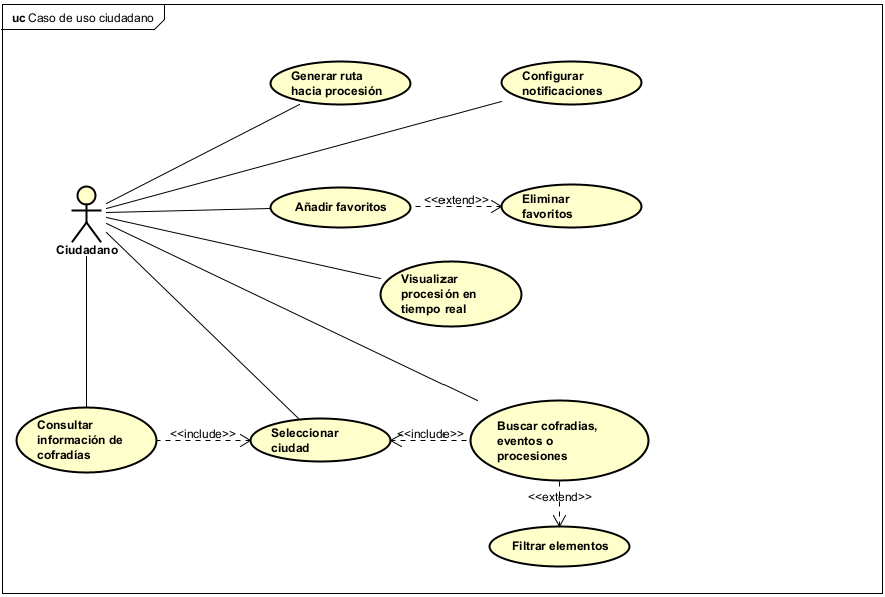
\includegraphics[width=0.6\textwidth]{imagenes/casoDeUsoCiudadano.png}
    \caption{Diagrama de caso de uso Ciudadano}
    \label{fig:casoUso1}
\end{figure}

\begin{figure}[H]
    \centering
    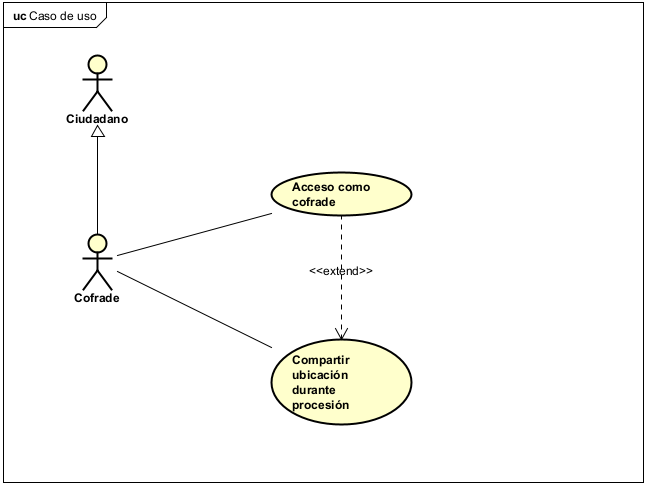
\includegraphics[width=0.6\textwidth]{imagenes/casoDeUsoCofrade.png}
    \caption{Diagrama de caso de uso Cofrade}
    \label{fig:casoUso2}
\end{figure}

\begin{figure}[H]
    \centering
    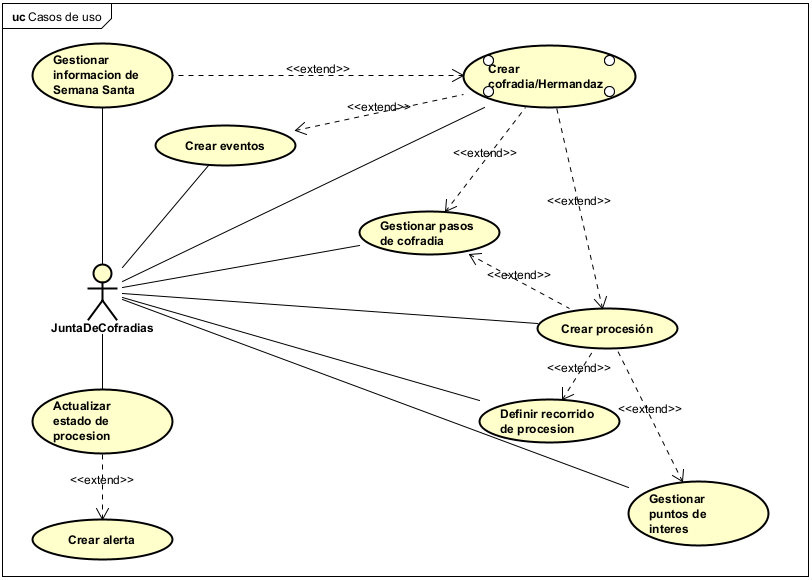
\includegraphics[width=0.6\textwidth]{imagenes/casoDeUsoJuntaDeCofradias.png}
    \caption{Diagrama de caso de uso Junta de Cofradías}
    \label{fig:casoUso3}
\end{figure}


\begin{figure}[H]
    \centering
    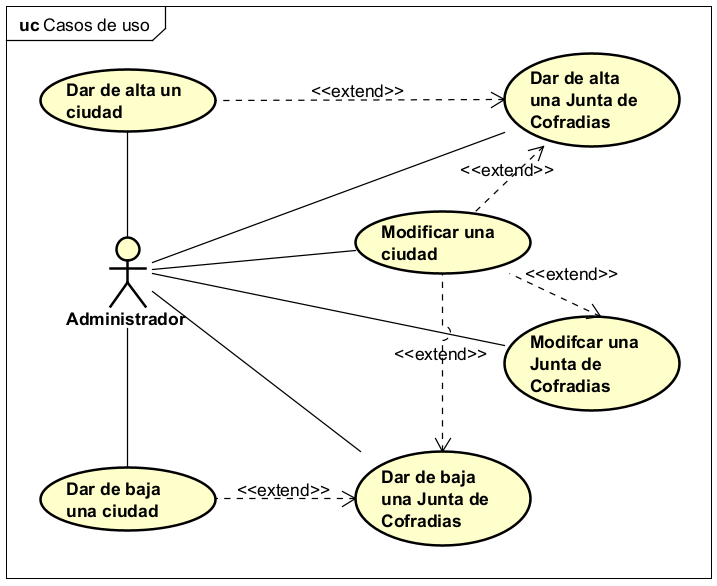
\includegraphics[width=0.6\textwidth]{imagenes/casoDeUsoAdministrador.png}
    \caption{Diagrama de caso de uso Administrador}
    \label{fig:casoUso4}
\end{figure}

En las siguientes tablas se exponen los cinco casos de uso más representativos del sistema, uno por cada rol implicado (ciudadano, cofrade, Junta de Cofradías y administrador), donde se detallan: el caso de uso, los actores que lo realizan, las precondiciones necesarias para iniciar el caso de uso, las postcondiciones que deben cumplirse al completarse, una secuencia base de pasos, secuencias alternativas que pueden darse durante la ejecución y los requisitos relacionados con el caso de uso. El resto de los casos de uso identificados, de carácter más secundario, se recogen en el Apéndice~\ref{cap:casos_de_uso_adicionales}.


\begin{table}[h!]
    \centering
    \renewcommand{\arraystretch}{1.5}

    \begin{tabular}{|p{4cm}|p{11cm}|}
        \hline
        \multicolumn{2}{|l|}{\textbf{Caso de uso: Visualizar procesión en tiempo real}}                                                             \\
        \hline
        \textbf{Resumen}                                                                                                                           & El usuario visualiza la posición actual de una procesión en el mapa. \\
        \hline
        \textbf{Actor}                                                                                                                             & Ciudadano                                                            \\
        \hline
        \textbf{Precondición}                                                                                                                      & La procesión está en curso El usuario tiene conexión a internet      \\
        \hline
        \textbf{Postcondición}                                                                                                                     & Se muestra la lista de cofradías con su información.                 \\
        \hline
        \multicolumn{2}{|l|}{\textbf{Secuencia Base}}                                                                                               \\
        \hline
        \multicolumn{2}{|p{15cm}|}{ [1] El usuario selecciona una procesión activa. }                                                               \\
        \hline
        \multicolumn{2}{|p{15cm}|}{ [2] El sistema muestra el mapa con el recorrido de la procesión. }                                              \\
        \hline
        \multicolumn{2}{|p{15cm}|}{ [3] El sistema actualiza la posición en tiempo real. }                                                          \\
        \hline
        \multicolumn{2}{|p{15cm}|}{ [4] El usuario puede interactuar con el mapa (zoom, desplazamiento). }                                          \\
        \hline
        \multicolumn{2}{|l|}{\textbf{Secuencia Alternativa}}                                                                                        \\
        \hline
        \multicolumn{2}{|p{15cm}|}{ [1.a.1] La procesión no está activa: El sistema muestra el recorrido planificado sin posición en tiempo real. } \\
        \hline
        \multicolumn{2}{|p{15cm}|}{ [3.a.1] Pérdida de conexión: El sistema muestra la última posición conocida. }                                  \\
        \hline
        \textbf{Requisitos Relacionados}                                                                                                           & RF-05, RF-14 y RF-16.                                                \\
        \hline
    \end{tabular}
    \caption{Caso de uso: Visualizar procesión en tiempo real}
\end{table}


\begin{table}[h!]
    \centering
    \renewcommand{\arraystretch}{1.5}

    \begin{tabular}{|p{4cm}|p{11cm}|}
        \hline
        \multicolumn{2}{|l|}{\textbf{Caso de uso: Compartir ubicación durante procesión}}                                                   \\
        \hline
        \textbf{Resumen}                                                                                                                   & Un cofrade comparte su ubicación en tiempo real durante una procesión.                                         \\
        \hline
        \textbf{Actor}                                                                                                                     & Cofrade                                                                                                        \\
        \hline
        \textbf{Precondición}                                                                                                              & El cofrade está registrado, el cofrade tiene permisos de ubicación y hay una procesión de su cofradía en curso \\
        \hline
        \textbf{Postcondición}                                                                                                             & La ubicación del cofrade se transmite al sistema.                                                              \\
        \hline
        \multicolumn{2}{|l|}{\textbf{Secuencia Base}}                                                                                       \\
        \hline
        \multicolumn{2}{|p{15cm}|}{ [1] El cofrade accede a la procesión activa de su cofradía. }                                           \\
        \hline
        \multicolumn{2}{|p{15cm}|}{ [2] El cofrade activa la opción de compartir ubicación. }                                               \\
        \hline
        \multicolumn{2}{|p{15cm}|}{ [3] El sistema solicita permisos de ubicación si no los tiene. }                                        \\
        \hline
        \multicolumn{2}{|p{15cm}|}{ [4] El cofrade concede los permisos. }                                                                  \\
        \hline
        \multicolumn{2}{|p{15cm}|}{ [5] El sistema comienza a transmitir la ubicación. }                                                    \\
        \hline
        \multicolumn{2}{|p{15cm}|}{ [6] El sistema muestra indicador de ubicación compartida. }                                             \\
        \hline
        \multicolumn{2}{|l|}{\textbf{Secuencia Alternativa}}                                                                                \\
        \hline
        \multicolumn{2}{|p{15cm}|}{ [4.a.1] El usuario deniega permisos: El sistema informa que no puede compartir ubicación sin permiso. } \\
        \hline
        \multicolumn{2}{|p{15cm}|}{ [2.a.1] Cancelación de la operación: El usuario desea cancelar la operacion. }                             \\
        \hline
        \multicolumn{2}{|p{15cm}|}{ [5.a.1] Pérdida de conexión: El sistema muestra la última posición conocida. }                          \\
        \hline
        \textbf{Requisitos Relacionados}                                                                                                   & RF-13 y RF-17.                                                                                                 \\
        \hline
    \end{tabular}
    \caption{Caso de uso: Compartir ubicación durante procesión}
\end{table}


\begin{table}[h!]
    \centering
    \renewcommand{\arraystretch}{1.5}

    \begin{tabular}{|p{4cm}|p{11cm}|}
        \hline
        \multicolumn{2}{|l|}{\textbf{Caso de uso: Crear alerta}}                                                         \\
        \hline
        \textbf{Resumen}                                                                                                & La Junta de Cofradías crea una alerta para informar a los usuarios sobre incidencias o información relevante. \\
        \hline
        \textbf{Actor}                                                                                                  & Junta de Cofradías                                                                                            \\
        \hline
        \textbf{Precondición}                                                                                           & El usuario tiene rol de Junta de Cofradías.                                                                   \\
        \hline
        \textbf{Postcondición}                                                                                          & La alerta queda creada y se envian notificaciones a los usuarios afectados.                                   \\
        \hline
        \multicolumn{2}{|l|}{\textbf{Secuencia Base}}                                                                    \\
        \hline
        \multicolumn{2}{|p{15cm}|}{ [1] El usuario accede al panel de gestion de alertas. }                              \\
        \hline
        \multicolumn{2}{|p{15cm}|}{ [2] El usuario selecciona crear nueva alerta. }                                      \\
        \hline
        \multicolumn{2}{|p{15cm}|}{ [3] El sistema muestra el formulario de creacion. }                                  \\
        \hline
        \multicolumn{2}{|p{15cm}|}{ [4] El usuario selecciona el tipo de alerta. }                                       \\
        \hline
        \multicolumn{2}{|p{15cm}|}{ [5] El usuario introduce titulo y mensaje de la alerta. }                            \\
        \hline
        \multicolumn{2}{|p{15cm}|}{ [6] El usuario selecciona la prioridad de la alerta. }                               \\
        \hline
        \multicolumn{2}{|p{15cm}|}{ [7] El usuario define fecha de expiracion (opcional). }                              \\
        \hline
        \multicolumn{2}{|p{15cm}|}{ [8] El usuario selecciona los destinatarios. }                                       \\
        \hline
        \multicolumn{2}{|p{15cm}|}{ [9] El usuario confirma la creacion. }                                               \\
        \hline
        \multicolumn{2}{|p{15cm}|}{ [10] El sistema crea la alerta y envia notificaciones. }                             \\
        \hline
        \multicolumn{2}{|l|}{\textbf{Secuencia Alternativa}}                                                             \\
        \hline
        \multicolumn{2}{|p{15cm}|}{ [4.a.1] Cancelación de la operación: El usuario desea cancelar la operacion. }          \\
        \hline
        \multicolumn{2}{|p{15cm}|}{ [5.a.1] Cancelación de la operación: El usuario desea cancelar la operacion. }          \\
        \hline
        \multicolumn{2}{|p{15cm}|}{ [6.a.1] Cancelación de la operación: El usuario desea cancelar la operacion. }          \\
        \hline
        \multicolumn{2}{|p{15cm}|}{ [7.a.1] Cancelación de la operación: El usuario desea cancelar la operacion. }          \\
        \hline
        \multicolumn{2}{|p{15cm}|}{ [8.a.1] Cancelación de la operación: El usuario desea cancelar la operacion. }          \\
        \hline
        \multicolumn{2}{|p{15cm}|}{ [9.a.1] Datos incompletos: El sistema muestra los campos requeridos. }               \\
        \hline
        \multicolumn{2}{|p{15cm}|}{ [10.a.1] Error al enviar notificaciones: El sistema reintenta y registra el error. } \\
        \hline
        \textbf{Requisitos Relacionados}                                                                                & RF-11, RF-12 y RF-26.                                                                                         \\
        \hline
    \end{tabular}
    \caption{Caso de uso: Crear alerta}
\end{table}

\begin{table}[h!]
    \centering
    \renewcommand{\arraystretch}{1.5}

    \begin{tabular}{|p{4cm}|p{11cm}|}
        \hline
        \multicolumn{2}{|l|}{\textbf{Caso de uso: Acceso como cofrade}}                                                                   \\
        \hline
        \textbf{Resumen}                                                                                                                 & Un usuario se registra en la aplicación como miembro de una cofradía. \\
        \hline
        \textbf{Actor}                                                                                                                   & Cofrade                                                               \\
        \hline
        \textbf{Precondición}                                                                                                            & El usuario no está registrado.                                        \\
        \hline
        \textbf{Postcondición}                                                                                                           & El usuario queda registrado y puede acceder a funciones de cofrade.   \\
        \hline
        \multicolumn{2}{|l|}{\textbf{Secuencia Base}}                                                                                     \\
        \hline
        \multicolumn{2}{|p{15cm}|}{ [1] El usuario selecciona la opción de registro. }                                                    \\
        \hline
        \multicolumn{2}{|p{15cm}|}{ [2] El sistema muestra el formulario de registro (Introducir código de acceso para dicha cofradía). } \\
        \hline
        \multicolumn{2}{|p{15cm}|}{ [3] El usuario introduce el código de acceso de la cofradía. }                                        \\
        \hline
        \multicolumn{2}{|p{15cm}|}{ [4] El sistema valida el código. }                                                                    \\
        \hline
        \multicolumn{2}{|p{15cm}|}{ [5] El sistema muestra mensaje informando del correcto acceso. }                                      \\
        \hline
        \multicolumn{2}{|l|}{\textbf{Secuencia Alternativa}}                                                                              \\
        \hline
        \multicolumn{2}{|p{15cm}|}{ [3.a.1] Cancelación de la operación: El usuario desea cancelar la operacion. }                           \\
        \hline
        \multicolumn{2}{|p{15cm}|}{ [5.a.1] Codigo inválido: El sistema muestra los errores de validación. }                              \\
        \hline
        \textbf{Requisitos Relacionados}                                                                                                 & RF-02.                                                                \\
        \hline
    \end{tabular}
    \caption{Caso de uso: Acceso como cofrade}
\end{table}

\begin{table}[h!]
    \centering
    \renewcommand{\arraystretch}{1.5}

    \begin{tabular}{|p{4cm}|p{11cm}|}
        \hline
        \multicolumn{2}{|l|}{\textbf{Caso de uso: Dar de alta ciudad}}                                                      \\
        \hline
        \textbf{Resumen}                                                                                                    & El administrador da de alta una nueva ciudad disponible en la aplicación.                                            \\
        \hline
        \textbf{Actor}                                                                                                      & Administrador                                                                                                         \\
        \hline
        \textbf{Precondición}                                                                                               & El usuario tiene rol de Administrador.                                                                               \\
        \hline
        \textbf{Postcondición}                                                                                              & La nueva ciudad queda disponible en el sistema.                                                                      \\
        \hline
        \multicolumn{2}{|l|}{\textbf{Secuencia Base}}                                                                       \\
        \hline
        \multicolumn{2}{|p{15cm}|}{ [1] El usuario accede al panel de administración. }                                     \\
        \hline
        \multicolumn{2}{|p{15cm}|}{ [2] El sistema muestra la lista de ciudades existentes. }                               \\
        \hline
        \multicolumn{2}{|p{15cm}|}{ [3] El usuario selecciona la opción de añadir ciudad. }                                 \\
        \hline
        \multicolumn{2}{|p{15cm}|}{ [4] El usuario introduce los datos de la nueva ciudad. }                                \\
        \hline
        \multicolumn{2}{|p{15cm}|}{ [5] El sistema valida y guarda la nueva ciudad. }                                       \\
        \hline
        \multicolumn{2}{|l|}{\textbf{Secuencia Alternativa}}                                                                \\
        \hline
        \multicolumn{2}{|p{15cm}|}{ [4.a.1] Cancelación de la operación: El usuario desea cancelar la operación. }          \\
        \hline
        \multicolumn{2}{|p{15cm}|}{ [5.a.1] Datos incompletos: El sistema muestra los campos requeridos. }                  \\
        \hline
        \textbf{Requisitos Relacionados}                                                                                    & RF-26.                                                                                                                \\
        \hline
    \end{tabular}
    \caption{Caso de uso: Dar de alta ciudad}
\end{table}

\section{Modelo de dominio}\label{cap:modelo_de_dominio}

En esta sección se detalla el diseño conceptual del sistema, incluyendo las entidades clave y sus relaciones. El modelo refleja la estructura lógica del dominio de la Semana Santa, garantizando una representación fiel de sus procesos, actores y reglas de negocio. Tras las correcciones indicadas por el tutor sobre la versión anterior del diagrama, y una segunda ronda de ajustes propios, se explican a continuación con más detalle las abstracciones incluidas en la Figura~\ref{fig:DiagramDomain}, la relación entre ellas y las decisiones de diseño tomadas para resolver los puntos que generaban confusión.

\clearpage
\begin{figure}[H]
\centering
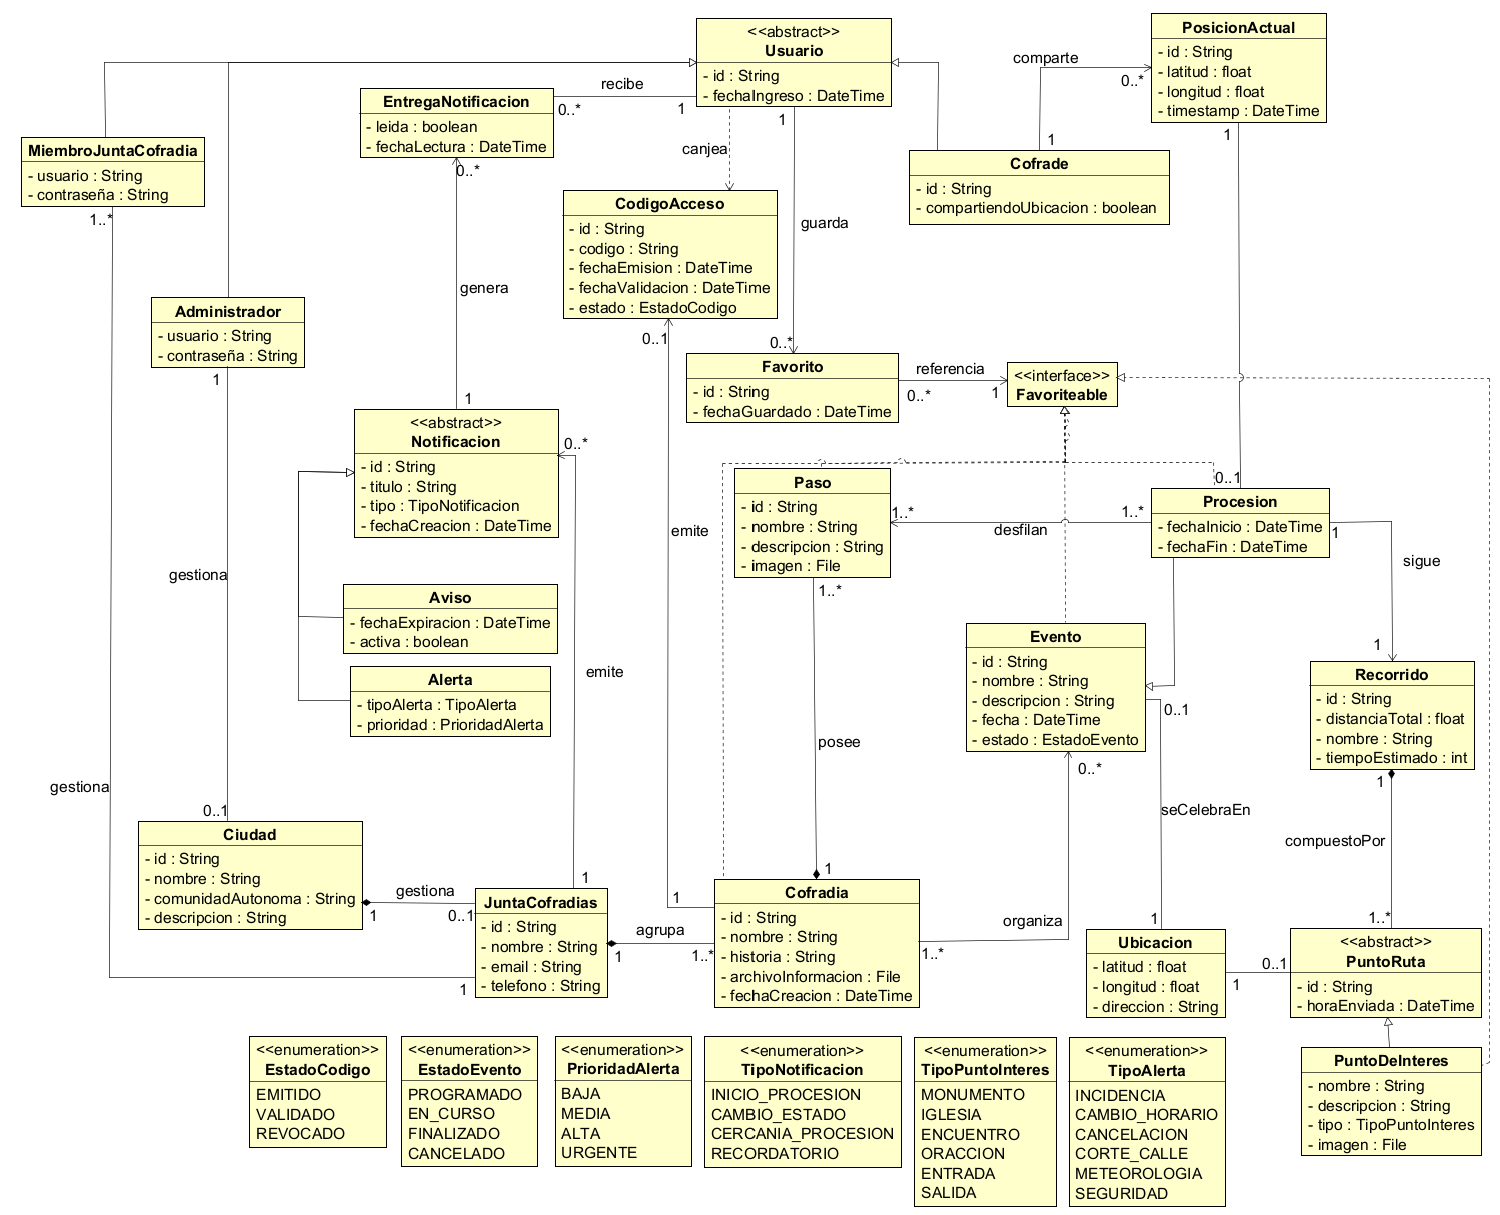
\includegraphics[width=1\textwidth,height=0.85\textheight,keepaspectratio]{imagenes/DiagramaDeDominio.png}
\caption{Diagrama de dominio del proyecto}
\label{fig:DiagramDomain}
\end{figure}

\subsection{Usuarios y roles}

En la versión anterior, todas las asociaciones relativas al usuario (compartir ubicación, guardar favoritos, canjear un código de acceso...) partían de una única clase \texttt{Usuario}, lo que generaba confusión porque algunas de esas asociaciones sólo tienen sentido para un cofrade. Para eliminarla, \texttt{Usuario} pasa a ser una clase abstracta con lo común a cualquier persona que usa la aplicación sin necesidad de registro (\texttt{id} y \texttt{fechaIngreso}, guardar \texttt{Favorito} y recibir \texttt{EntregaNotificacion}), de la que \texttt{Cofrade} hereda añadiendo \texttt{compartiendoUbicacion} y la posibilidad de compartir su \texttt{PosicionActual}.

\texttt{Administrador} y \texttt{MiembroJuntaCofradia} se modelan como clases independientes, al margen de la jerarquía de \texttt{Usuario}: ambas representan cuentas de acceso a paneles de gestión (con su propio \texttt{usuario} y \texttt{contraseña}), y no perfiles de la aplicación pública, por lo que su forma de autenticarse no tiene relación con la de un ciudadano o un cofrade. \texttt{Administrador} administra las \texttt{Ciudad} y las \texttt{JuntaCofradias} del sistema (RF-26 y RF-34); \texttt{MiembroJuntaCofradia} es quien, en representación de una \texttt{JuntaCofradias}, gestiona su contenido (cofradías, eventos, procesiones, alertas...), ya que la propia \texttt{JuntaCofradias} es una entidad organizativa y no una persona que inicia sesión.

El canje de un \texttt{CodigoAcceso} se modela como una dependencia de \texttt{Usuario} hacia \texttt{CodigoAcceso} (\textit{canjea}) y no como una asociación permanente: representa la acción de introducir el código, tras la cual, si es válido, el usuario pasa a ser un \texttt{Cofrade}. El resultado de esa acción queda registrado en el propio \texttt{CodigoAcceso}, a través de su \texttt{estado} (\texttt{EstadoCodigo}: emitido, validado o revocado) y su \texttt{fechaValidacion}.

\subsection{Ciudad y Junta de Cofradías}

Una \texttt{Ciudad} está gestionada como máximo por una \texttt{JuntaCofradias} (multiplicidad \texttt{0..1}), y no por varias: en el dominio de la aplicación cada ciudad cuenta con una única junta de cofradías de referencia (RI-10), que agrupa a su vez todas las \texttt{Cofradia} de esa localidad (\texttt{1..*}) y cuenta con uno o varios \texttt{MiembroJuntaCofradia} que la gestionan desde el panel correspondiente.

\subsection{Cofradías, eventos y procesiones}

Cada \texttt{Cofradia} posee uno o varios \texttt{Paso} (relación de composición, ya que un paso no existe sin la cofradía a la que pertenece) y organiza uno o varios \texttt{Evento}. La relación \textit{organiza} es de muchos a muchos: un mismo evento puede estar organizado conjuntamente por varias cofradías (por ejemplo, una procesión general o un acto conjunto de Semana Santa en el que participan distintas hermandades), y no únicamente por una.

Un \texttt{Paso} puede desfilar en más de una \texttt{Procesion} (por ejemplo, en la procesión propia de su cofradía y en una procesión conjunta como una general o un vía crucis), de ahí que la relación \textit{desfilan} sea de muchos a muchos. Cada \texttt{Procesion} está vinculada a un \texttt{Evento} y sigue un \texttt{Recorrido} (\textit{sigue}), compuesto a su vez por distintos \texttt{PuntoRuta}, clase abstracta de la que heredan \texttt{Ubicacion} y \texttt{PuntoDeInteres}.

La \texttt{Procesion} no incorpora un atributo propio de descripción: su información descriptiva se obtiene a través del \texttt{Evento} al que está vinculada (que sí tiene \texttt{descripcion}) y de la \texttt{historia} de la \texttt{Cofradia} que lo organiza, evitando así duplicar el mismo dato en dos sitios. Por su parte, \texttt{Evento} se asocia a una \texttt{Ubicacion} (\textit{seCelebraEn}) que recoge la latitud, longitud y dirección donde tiene lugar (un pregón, un traslado, un concierto...), reutilizando la misma clase que ya se emplea para los puntos de un recorrido, en lugar de duplicar un atributo de dirección suelto.

Por coherencia con el resto de elementos que pueden marcarse como favoritos, la interfaz \texttt{Favoriteable} la realizan \texttt{Evento}, \texttt{Procesion} y \texttt{Cofradia}, que son los tres tipos de elemento que un usuario puede marcar como favorito según el requisito RF-12.

\subsection{Geolocalización en tiempo real}

Para la geolocalización en tiempo real, un \texttt{Cofrade} puede compartir su posición durante una procesión, lo que genera instancias de \texttt{PosicionActual}. A partir de las distintas posiciones compartidas por los cofrades que participan en una misma procesión, el backend calcula una única \texttt{PosicionActual} agregada, que es la que queda asociada a la \texttt{Procesion} como su posición en vivo (\textit{procesionEnVivo}) y la que consultan el resto de usuarios de la aplicación. Es decir, de cara al usuario que sigue la procesión, ésta se representa como un único punto (el resultado del cálculo), y no como el conjunto de puntos individuales de cada cofrade ni como un trazo continuo; esta decisión de diseño quedará confirmada con el resto del equipo antes de la implementación.

\subsection{Notificaciones, avisos y alertas}

La comunicación con los usuarios se modela mediante la clase abstracta \texttt{Notificacion}, de la que heredan \texttt{Aviso} y \texttt{Alerta}. Ambas comparten el atributo \texttt{tipo} (\texttt{TipoNotificacion}), que indica el origen o motivo concreto de la notificación: \texttt{INICIO\_PROCESION}, \texttt{CAMBIO\_ESTADO} y \texttt{CERCANIA\_PROCESION} corresponden a notificaciones que el sistema genera automáticamente cuando cambia el estado de una cofradía, evento o procesión marcada como favorita por el usuario (por ejemplo, ``comienza la procesión X'' cuando ésta pasa a estado \texttt{EN\_CURSO}), mientras que \texttt{RECORDATORIO} se emite un tiempo antes del inicio previsto. Esta generación automática no requiere que la \texttt{JuntaCofradias} cree la notificación a mano: basta con que el sistema detecte el cambio sobre un elemento favorito para generarla.

La diferencia entre \texttt{Aviso} y \texttt{Alerta} es de naturaleza, no de origen: el \texttt{Aviso} es un mensaje puramente informativo con una fecha de expiración (por ejemplo, un recordatorio o la confirmación de un cambio de estado), mientras que la \texttt{Alerta} se reserva para incidencias que requieren la atención del usuario, e incorpora un \texttt{tipoAlerta} (incidencia, cambio de horario, cancelación, corte de calle, meteorología o seguridad) y una \texttt{prioridad}. Ambas pueden generarse tanto de forma automática (a partir de un cambio de estado) como manualmente por parte de un \texttt{MiembroJuntaCofradia} (RF-27), en particular en el caso de las alertas de incidencias o cortes de calle, que no pueden deducirse solas a partir del estado de una procesión.

Cada notificación entregada a un usuario se registra mediante una \texttt{EntregaNotificacion}, que almacena si ha sido leída y en qué momento, evitando así duplicar la notificación en sí para cada destinatario: una misma \texttt{Notificacion} puede generar tantas instancias de \texttt{EntregaNotificacion} como usuarios la reciban (\texttt{0..*}).

\subsection{Acceso al modo cofrade}

Por último, el acceso al modo cofrade se controla mediante la clase \texttt{CodigoAcceso}: la \texttt{JuntaCofradias} emite los códigos, y un \texttt{Usuario} los canjea para pasar a ser \texttt{Cofrade}. De forma similar, los elementos marcados como favoritos por un usuario (cofradías, eventos o procesiones) se representan mediante la clase \texttt{Favorito}, que hace referencia a cualquier elemento que implemente la interfaz \texttt{Favoriteable}.

\subsection{Modelo de dominio detallado}

Con el modelo de dominio y los diagramas de secuencia anteriores, construimos un modelo de dominio extendido (Figura ~\ref{fig:DiagramDomainDetail}) con los métodos a implementar.

\begin{figure}[H]
\centering
\includegraphics[width=1\textwidth,height=0.85\textheight,keepaspectratio]{imagenes/DiagramaDeDominioDetallado.png}
\caption{Diagrama de dominio detallado del proyecto}
\label{fig:DiagramDomainDetail}
\end{figure}

\subsection{Realización en análisis de los casos de uso}

En este apartado se mostrarán los diagramas de secuencia obtenidos del análisis a partir de los casos de uso mencionados anteriormente. Se han excluido de esta sección las secuencias alternativas de cancelar con el fin de simplificar los diagramas.

Para el caso de uso \textit{Visualizar procesión en tiempo real} (Figura~\ref{fig:secVisualizarProcesion}), el ciudadano selecciona una procesión activa y el sistema obtiene la instancia de \texttt{Procesion} correspondiente, junto con su recorrido planificado, y se suscribe a las actualizaciones de su posición actual. Mientras la procesión está en curso, el sistema recalcula sobre el recorrido el tramo ya realizado y el tramo restante en función de la posición recibida, para mantener el mapa del usuario actualizado.

\begin{figure}[H]
\centering
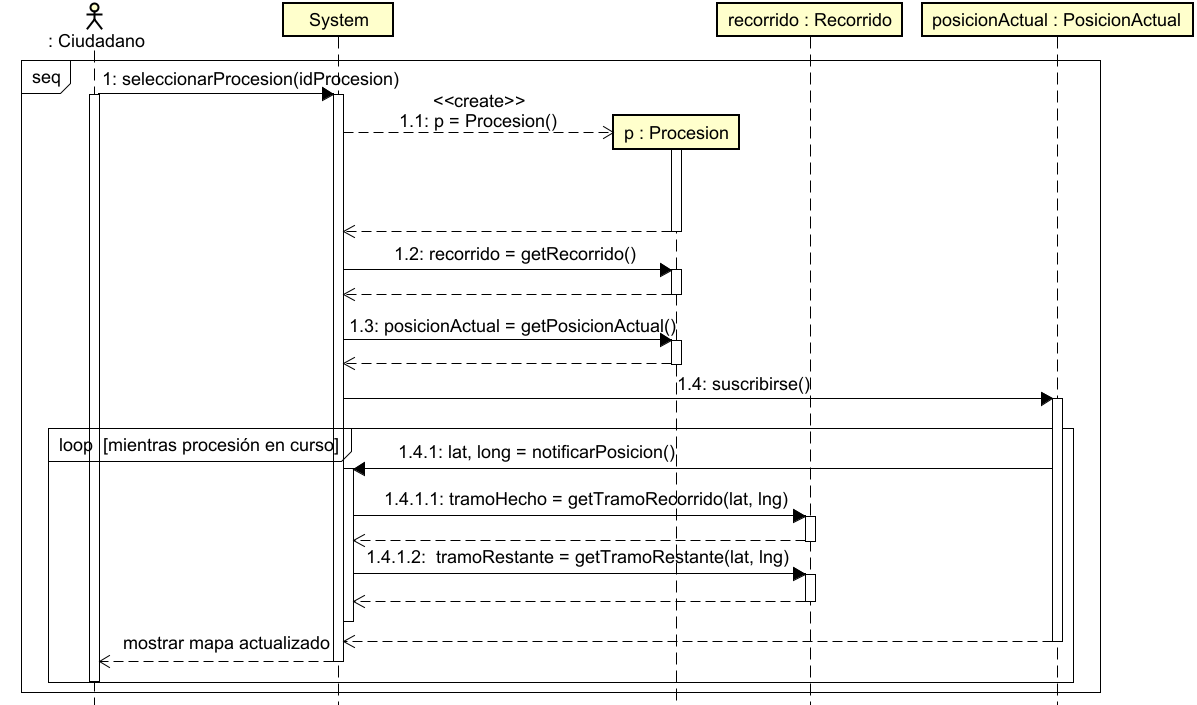
\includegraphics[width=1\textwidth,keepaspectratio]{imagenes/DSCasoUsoVerProcesion.png}
\caption{Diagrama de secuencia del CU ``Visualizar procesión en tiempo real''}
\label{fig:secVisualizarProcesion}
\end{figure}

En el caso de uso \textit{Compartir ubicación durante procesión} (Figura~\ref{fig:secCompartirUbicacion}), el cofrade accede a la procesión activa de su cofradía y activa la opción de compartir su ubicación. El sistema solicita los permisos de localización si no los tiene concedidos: si el cofrade los deniega, se le informa de que no es posible compartir la ubicación sin permiso; si los concede, el sistema comienza a actualizar de forma periódica la posición del cofrade mientras la procesión sigue en curso.

\begin{figure}[H]
\centering
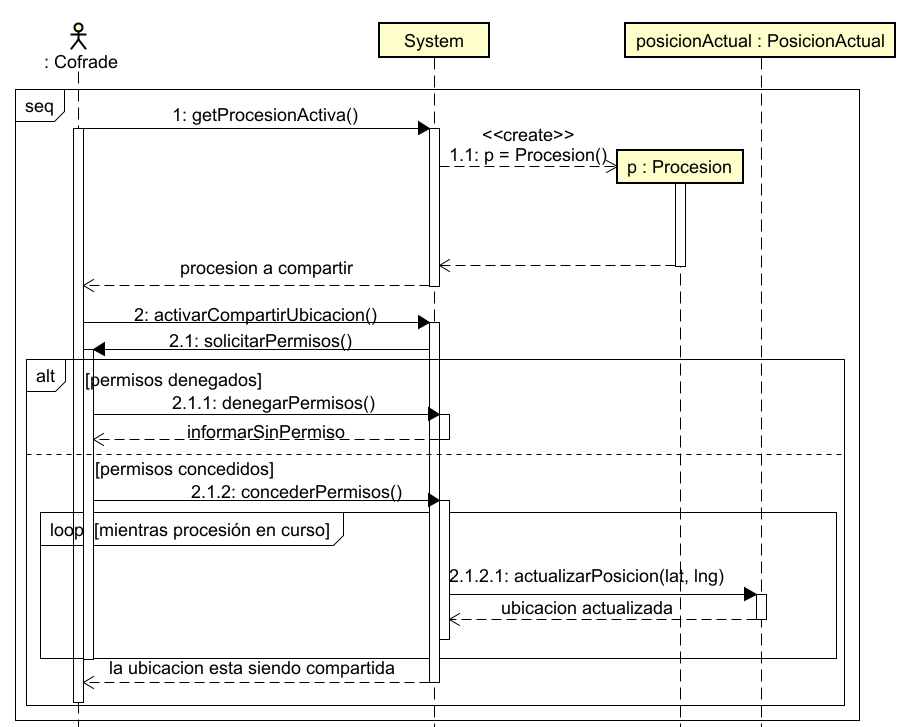
\includegraphics[width=1\textwidth,keepaspectratio]{imagenes/DSCasoUsoCompartirUbi.png}
\caption{Diagrama de secuencia del CU ``Compartir ubicación durante procesión''}
\label{fig:secCompartirUbicacion}
\end{figure}

En el caso de uso \textit{Acceso como cofrade} (Figura~\ref{fig:secAccesoCofrade}), el usuario selecciona la opción de registro y el sistema le muestra el formulario correspondiente. Al introducir el código de acceso de su cofradía, el sistema obtiene el \texttt{CodigoAcceso} correspondiente y lo valida, informando al usuario del acceso correcto o de un error de validación según el resultado.

\begin{figure}[H]
\centering
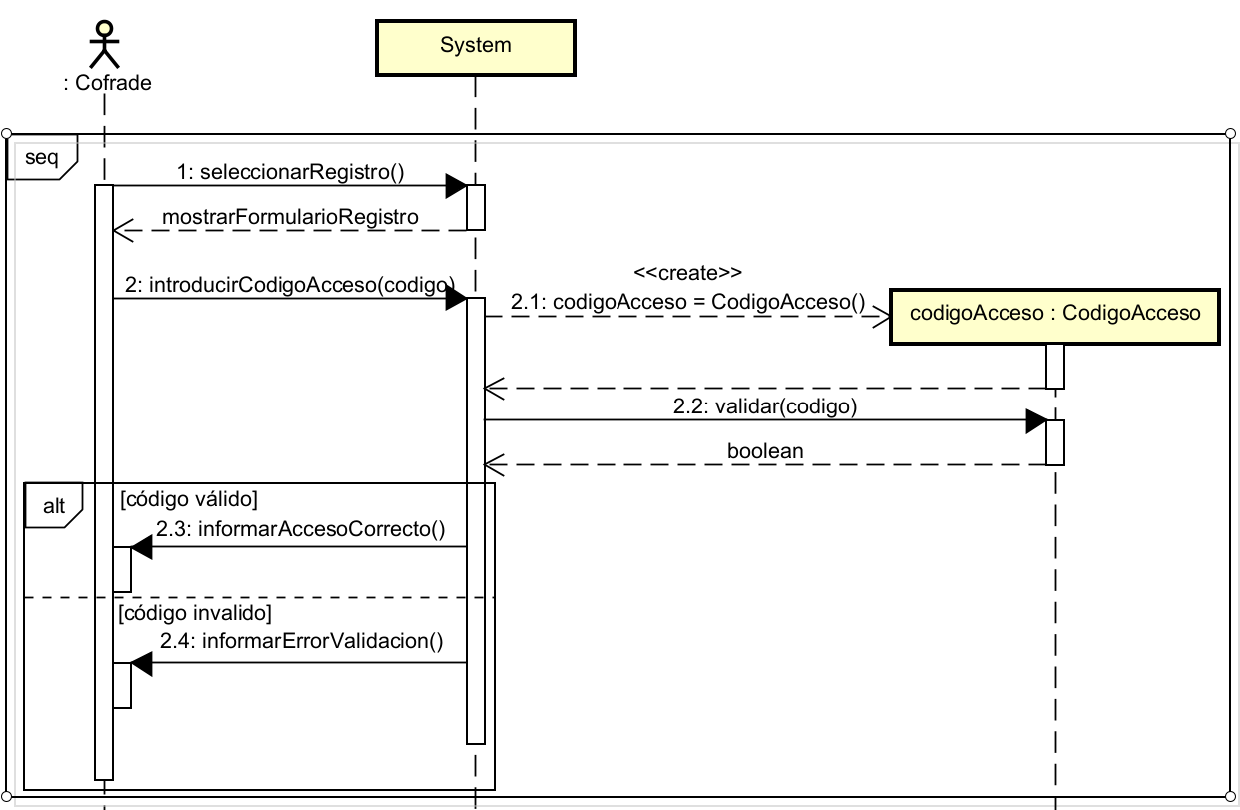
\includegraphics[width=1\textwidth,keepaspectratio]{imagenes/DSCasoUsoAccesoCofrade.png}
\caption{Diagrama de secuencia del CU ``Acceso como cofrade''}
\label{fig:secAccesoCofrade}
\end{figure}

En el caso de uso \textit{Dar de alta ciudad} (Figura~\ref{fig:secAltaCiudad}), el administrador accede al panel de administración, donde el sistema le muestra la lista de ciudades existentes, y selecciona la opción de añadir una nueva ciudad. Tras introducir los datos, el sistema construye la instancia de \texttt{Ciudad} correspondiente y valida los datos introducidos, repitiendo la solicitud hasta que estos son válidos, momento en el que la ciudad queda dada de alta.

\begin{figure}[H]
\centering
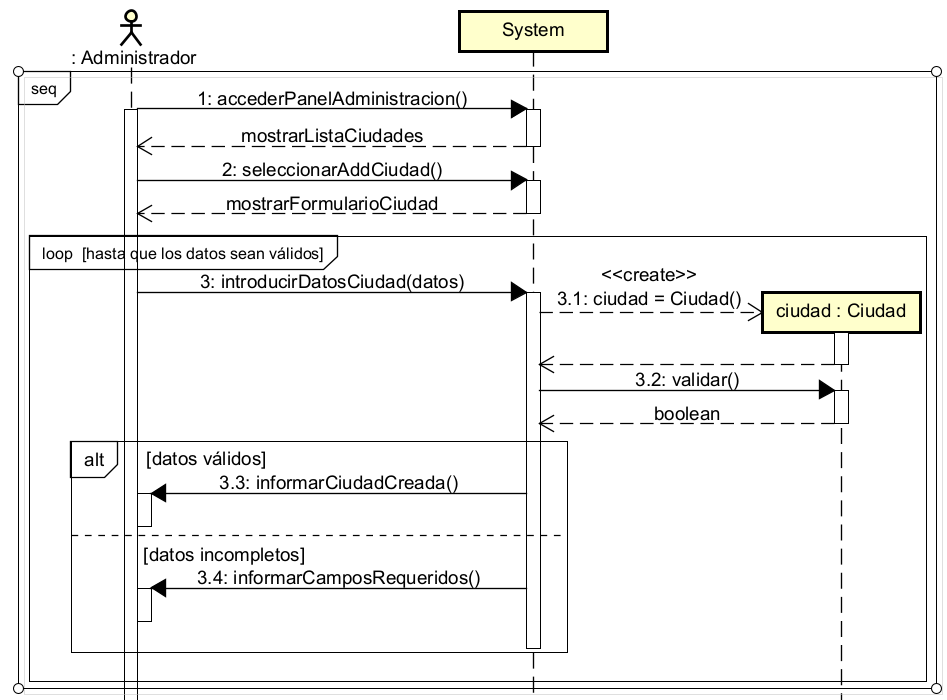
\includegraphics[width=1\textwidth,keepaspectratio]{imagenes/DSCasoUsoCrearCiudad.png}
\caption{Diagrama de secuencia del CU ``Dar de alta ciudad''}
\label{fig:secAltaCiudad}
\end{figure}

% TODO: diagramas de secuencia pendientes de añadir - Editar ciudad, Dar de baja ciudad y Crear alerta.


\chapter{Descripción de las iteraciones}\label{cap:iteraciones}
\section{1ª Iteración}\label{cap:1_iteracion}

\subsection{Analisís}

\subsection{Diseño}

Antes de comenzar la implementación de esta primera iteración ha sido necesario tomar una serie de decisiones de diseño que condicionan el resto del proyecto: qué tecnologías se van a usar, cómo se organiza el código, cómo se guardan los datos y qué soluciones ya conocidas (patrones de diseño) conviene aplicar. Estas decisiones se explican a continuación con el detalle suficiente para que puedan entenderse sin conocimientos previos de React Native o Firebase, ya que sientan la base para el resto de iteraciones del proyecto.

\subsubsection{Decisiones tecnológicas}

Para el cliente\footnote{Cliente: en una arquitectura cliente-servidor, es la parte del sistema con la que interactúa directamente el usuario; en este caso, la propia aplicación instalada en el teléfono móvil.} móvil se ha optado por \textbf{React Native} \cite{reactnative}, un \emph{framework}\footnote{Framework: conjunto de herramientas y bibliotecas de código que facilitan el desarrollo de un tipo concreto de aplicación, proporcionando una estructura base sobre la que trabajar.} que permite escribir una única aplicación y ejecutarla tanto en Android como en iOS, en lugar de programar dos aplicaciones nativas independientes (una en Kotlin/Java para Android y otra en Swift para iOS). Se descarta el desarrollo nativo duplicado por dos motivos: el requisito RNF-07 exige que la aplicación funcione en ambas plataformas, y al tratarse de un proyecto desarrollado por una única persona, mantener y probar dos bases de código distintas multiplicaría el tiempo de desarrollo sin aportar ninguna ventaja funcional. Además, React Native dispone de librerías ya probadas para los dos puntos más críticos del sistema: la integración con mapas (\texttt{react-native-maps}) y el acceso a la geolocalización del dispositivo (\texttt{expo-location} o \texttt{react-native-geolocation-service}).

Como \emph{backend}\footnote{Backend: la parte del sistema que no ve el usuario directamente, encargada de almacenar los datos, gestionar la lógica de negocio y responder a las peticiones que le hace el cliente.} se ha optado por \textbf{Firebase} \cite{firebase}, una plataforma de Google que se ofrece como \emph{Backend-as-a-Service} (BaaS): en lugar de programar un servidor propio, se contratan una serie de servicios ya construidos (base de datos, autenticación de usuarios, almacenamiento de ficheros, envío de notificaciones) a los que la aplicación se conecta directamente. Se descarta programar un backend a medida porque Firebase ya resuelve de forma nativa todo lo anterior y, sobre todo, porque su base de datos (Cloud Firestore \cite{firestore}) permite que varios dispositivos vean los mismos datos actualizados en tiempo real sin que el equipo de desarrollo tenga que programar esa sincronización a mano: la aplicación simplemente se ``suscribe'' a los datos que le interesan y Firebase le avisa automáticamente cada vez que cambian (este mecanismo se denomina \emph{listener}, y se explica con más detalle en el apartado de patrones de diseño). Esta decisión es coherente con el riesgo ``Problemas con Firebase/base de datos'' identificado en la planificación (Sección~\ref{cap:analisisRiesgos}) y con el requisito RNF-08, que exige actualizar la posición de una procesión cada 30 segundos como mínimo.

Para los mapas se mantiene \textbf{Google Maps Platform} \cite{googlemapsapi}, ya justificado en el estado de la cuestión (Sección~1.3.2), por ser la solución de mapas más extendida y con mejor documentación. La contingencia prevista ante el riesgo ``Problemas con la integración de Google Maps'' (Sección~\ref{cap:analisisRiesgos}) sigue siendo migrar a OpenStreetMap \cite{openstreetmap} o Mapbox si en la práctica surgen problemas de cuota o de coste.

\subsubsection{Arquitectura del sistema}

La arquitectura de un sistema describe, a grandes rasgos, en qué piezas se divide y cómo se comunican entre sí. En este proyecto se ha definido una arquitectura \textbf{cliente-servidor sin servidor intermedio propio}: la aplicación React Native (el cliente) se comunica directamente con los SDK\footnote{SDK (\emph{Software Development Kit}): conjunto de herramientas que proporciona un servicio (en este caso, Firebase o Google Maps) para que otras aplicaciones puedan integrarse con él fácilmente, sin tener que hablar directamente con sus servidores a bajo nivel.} oficiales de Firebase (Authentication, Cloud Firestore, Cloud Messaging y Storage) y de Google Maps Platform (Maps SDK y Directions API). Es importante notar que no existe una capa de API REST\footnote{API REST: forma habitual de comunicación entre un cliente y un servidor propio, en la que el cliente pide o envía datos a través de peticiones HTTP a unas direcciones (\emph{endpoints}) definidas por el propio equipo de desarrollo. Al no tener servidor propio, esta capa no es necesaria en este proyecto.} propia entre el cliente y el servidor, como sí ocurriría si se hubiese optado por programar un backend a medida: es Firebase quien ya expone esa comunicación a través de su SDK. Internamente, el SDK de Firebase abre un canal de comunicación permanente con los servidores de Google (una conexión en tiempo real basada en HTTP/2, la misma tecnología que usa HTTPS) por la que viajan tanto las peticiones de lectura y escritura como los avisos de los \emph{listeners}; el SDK de Google Maps Platform, en cambio, solo se comunica puntualmente mediante peticiones HTTPS convencionales (por ejemplo, al calcular una ruta con la Directions API). En ambos casos es el propio SDK quien gestiona la conexión, la autenticación y la reconexión ante una pérdida de red, sin que la aplicación tenga que programar nada de eso.

\paragraph{Estructura del front-end}

Dentro del propio cliente, el código se organiza siguiendo una \textbf{arquitectura en capas} \cite{sommerville2015}: el proyecto se divide en varios grupos de carpetas (o \emph{paquetes}), cada uno con una responsabilidad concreta, de forma que cada capa solo puede depender de la capa inmediatamente inferior y nunca al revés. Esta regla se sigue para que un cambio en una capa concreta (por ejemplo, cambiar de Firebase a otro proveedor de datos) afecte al menor número posible de partes del código, y para poder probar cada capa de forma aislada. Las cuatro capas definidas son:

\begin{itemize}
    \item \textbf{UI} (\texttt{screens}, \texttt{components}, \texttt{navigation}): las pantallas que ve el usuario, agrupadas por su rol (ciudadano, cofrade, junta de cofradías, administrador), siguiendo los cuatro diagramas de casos de uso del Capítulo~\ref{cap:analisis}; los componentes visuales reutilizables entre pantallas (por ejemplo, la tarjeta con la información de una cofradía); y la navegación entre pantallas.
    \item \textbf{Application} (\texttt{context}, \texttt{hooks}): el estado que se comparte entre varias pantallas a la vez, como la sesión del usuario, su rol activo, la ciudad seleccionada o si está compartiendo su ubicación en ese momento.
    \item \textbf{Data} (\texttt{services}, \texttt{models}): un servicio por cada tipo de información del dominio (\texttt{cofradiaService}, \texttt{procesionService}, \texttt{geoService}, \texttt{notificationService}...) que es el único responsable de hablar con Firebase y con Google Maps, además de los tipos de datos que describen cómo es cada objeto (una cofradía, una procesión...) dentro de la aplicación.
    \item \textbf{Infrastructure} (\texttt{firebase}, \texttt{maps}): la configuración e inicialización de los SDK externos, es decir, el código mínimo necesario para que el resto de la aplicación pueda empezar a usar Firebase y Google Maps.
\end{itemize}

La Figura~\ref{fig:disenoPaquetes} muestra esta organización en forma de diagrama de paquetes, donde las flechas discontinuas indican qué paquete depende de (necesita) cuál.

\begin{figure}[H]
    \centering
    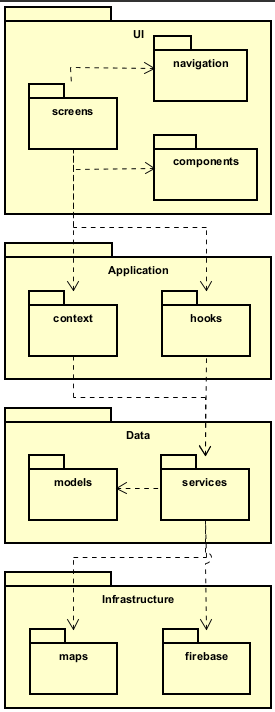
\includegraphics[width=0.45\textwidth]{imagenes/Dragrama de aplicacion front-end.png}
    \caption{Diagrama de paquetes de la aplicación cliente}
    \label{fig:disenoPaquetes}
\end{figure}

\paragraph{Estructura del back-end}

Como se ha explicado, el back-end de este proyecto no incluye código propio, sino que se apoya íntegramente en los siguientes servicios de Firebase:

\begin{itemize}
    \item \textbf{Firebase Authentication}: servicio que crea y gestiona la sesión de los usuarios con un rol elevado (cofrade, junta de cofradías, administrador), sin que el proyecto tenga que programar ni almacenar contraseñas por su cuenta. El ciudadano no necesita registrarse ni iniciar sesión en ningún momento: puede consultar procesiones, ver el mapa y recibir notificaciones sin tener ningún tipo de cuenta. Solo cuando un usuario introduce un código de acceso válido (colección \texttt{codigosAcceso}, ver apartado \nameref{sec:disenoBD}) se crea su sesión de Firebase Authentication y se le asigna el rol correspondiente.
    \item \textbf{Cloud Firestore}: la base de datos del proyecto. Guarda toda la información en las colecciones \texttt{ciudades}, \texttt{cofradias}, \texttt{eventos}, \texttt{procesiones}, \texttt{recorridos}, \texttt{usuarios} y \texttt{notificaciones} (el diseño completo de estas colecciones se explica en el apartado \nameref{sec:disenoBD} de esta misma sección).
    \item \textbf{Firebase Storage}: espacio de almacenamiento en la nube donde se guardan las imágenes de los pasos de cada cofradía, ya que este tipo de archivo no se guarda de forma eficiente dentro de la base de datos.
    \item \textbf{Cloud Messaging} \cite{firebasefcm}: servicio que permite enviar notificaciones \emph{push} (avisos que llegan al teléfono del usuario aunque no tenga la aplicación abierta en ese momento), usado para las alertas y avisos que publican las Juntas de Cofradías (RF-13, RF-14, RF-27).
\end{itemize}

\paragraph{Diagrama de despliegue}

Un diagrama de despliegue representa, de forma física, dónde se ejecuta cada parte del sistema y cómo se comunican entre sí esos entornos. La Figura~\ref{fig:disenoDespliegue} recoge el despliegue completo de este proyecto: el dispositivo móvil ejecuta la aplicación React Native, que se comunica mediante el protocolo HTTPS\footnote{HTTPS: versión segura (cifrada) del protocolo HTTP, usado habitualmente para la comunicación entre aplicaciones y servicios en internet.} tanto con Firebase (autenticación, base de datos, almacenamiento y notificaciones) como con Google Maps Platform (visualización de mapas y cálculo de rutas). Puede observarse que no existe ningún nodo de base de datos local: el requisito RNF-03 (disponibilidad de la información estática sin conexión a internet) queda cubierto por la caché\footnote{Caché: copia local y temporal de unos datos, guardada en el propio dispositivo, que permite seguir accediendo a ellos aunque se pierda la conexión a internet.} que Cloud Firestore guarda automáticamente en el dispositivo, sin que sea necesario implementar una base de datos local adicional como haría, por ejemplo, una aplicación Android nativa con Room. Este enfoque es más sencillo que el que sigue otro TFG de la escuela centrado en el funcionamiento sin conexión, el de Llorente Pérez~\cite{marioTFG}: su aplicación permite completar toda una actividad sin conexión a internet, guardando los datos en el propio dispositivo hasta poder enviarlos más tarde, porque está pensada para practicarse en el medio natural, donde puede no haber cobertura durante horas. En este proyecto, en cambio, las procesiones de Semana Santa transcurren en entornos urbanos con cobertura de red prácticamente garantizada, por lo que no hace falta un mecanismo tan complejo: basta con que la información estática (RNF-03) quede disponible sin conexión, que es justo lo que ya ofrece la caché de Firestore.

\begin{figure}[H]
    \centering
    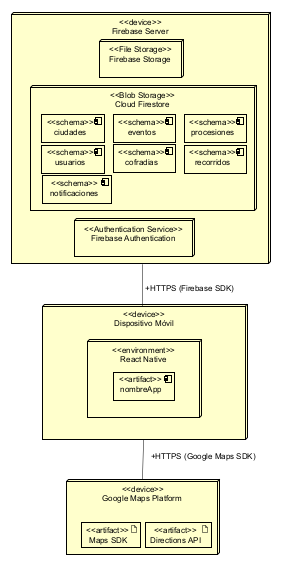
\includegraphics[width=0.45\textwidth]{imagenes/Diagrama de despliegue.png}
    \caption{Diagrama de despliegue de la aplicación}
    \label{fig:disenoDespliegue}
\end{figure}

\subsubsection{Diseño de la base de datos}\label{sec:disenoBD}

A diferencia de una base de datos relacional tradicional (como MySQL), organizada en tablas con filas y columnas relacionadas mediante claves, Cloud Firestore es una base de datos \textbf{NoSQL} \cite{nosql}\footnote{NoSQL: familia de bases de datos que no organiza la información en tablas relacionadas, sino en otras estructuras --en este caso, documentos agrupados en colecciones-- más flexibles para datos que cambian de forma o que se leen con mucha frecuencia en tiempo real.} de tipo documental: la información se organiza en \emph{colecciones} (agrupaciones de elementos del mismo tipo, similar a una carpeta) que contienen \emph{documentos} (cada elemento individual, similar a un fichero, con sus propios campos de datos). El modelo de dominio de la Figura~\ref{fig:DiagramDomain} se ha traducido a esta estructura de colecciones y subcolecciones (colecciones anidadas dentro de un documento concreto) siguiendo estas decisiones:

\begin{itemize}
    \item \texttt{pasos} y \texttt{puntosRuta} se modelan como \textbf{subcolecciones} de \texttt{cofradias} y \texttt{recorridos} respectivamente, porque siempre se consultan junto a su documento padre (por ejemplo, los pasos de una cofradía concreta) y nunca de forma independiente.
    \item \texttt{posicionActual} se modela como una \textbf{subcolección con un único documento} (\texttt{procesiones/\{id\}/posicionActual/actual}) en lugar de como un campo dentro del propio documento de la procesión, para que estas escrituras frecuentes de posición no afecten a los datos más estables de la procesión (horario, recorrido, pasos), que rara vez cambian. Este documento se sobrescribe cada vez que llega una nueva posición GPS. Cuando varios cofrades comparten su ubicación simultáneamente durante la misma procesión, sus posiciones se agregan y se escriben en modo \emph{batch} sobre este documento único, en lugar de realizar una escritura independiente por cada actualización individual, reduciendo así el número de operaciones sobre Firestore y, con ello, el consumo de ancho de banda y el coste asociado. El cliente se suscribe a este documento mediante un \emph{listener} en tiempo real (en vez de estar preguntando repetidamente si hay novedades, es Firestore quien avisa a la aplicación en cuanto el documento cambia), cumpliendo el requisito RNF-08 sin necesidad de implementar servidores de sockets propios. Al tratarse de un único documento por procesión que se sobrescribe con la posición agregada, el cliente recibe una sola actualización por cambio de posición en lugar de un flujo continuo de actualizaciones parciales por cada cofrade, evitando así problemas de parpadeo o sobrecarga en el mapa.
    \item \texttt{favoritos} no se guarda en Firestore, sino de forma local en el propio dispositivo (por ejemplo, con \texttt{AsyncStorage}), ya que el ciudadano no tiene cuenta ni sesión en la que persistir esta información en el servidor; únicamente se guarda el identificador de la cofradía o procesión marcada como favorita.
    \item \texttt{codigosAcceso} (subcolección de \texttt{cofradias}) y \texttt{notificacionesEntregadas} (subcolección de \texttt{usuarios}, que registra si un usuario ha leído cada notificación), estas sí como subcolecciones de Firestore, guardan únicamente una \textbf{referencia} (el identificador) a la cofradía, procesión, usuario o notificación correspondiente, en lugar de copiar todos sus datos, para evitar tener la misma información duplicada en varios sitios y que se desactualice.
    \item La colección \texttt{usuarios} solo contiene los perfiles de rol elevado (cofrade, junta de cofradías, administrador): el ciudadano no se registra, por lo que no genera ningún documento en Firestore para poder usar la aplicación. Un usuario obtiene uno de estos roles al introducir un \textbf{código de acceso} válido, gestionado en la subcolección \texttt{cofradias/\{id\}/codigosAcceso} (con estados \texttt{EMITIDO}, \texttt{VALIDADO} y \texttt{REVOCADO}); en ese momento se crea su sesión de Firebase Authentication y su documento en \texttt{/usuarios/\{id\}}, con el rol guardado como campo y comprobado mediante las reglas de seguridad de Firestore, mecanismo que cubre el requisito RNF-05 (control de acceso diferenciado por rol). Cada código de acceso lleva además una \textbf{referencia a la cofradía} que lo emite, de forma que un cofrade que valida su código queda automáticamente vinculado a esa cofradía y puede compartir su ubicación en tiempo real durante las procesiones en las que participa, que es la única acción que el modelo de dominio le permite realizar directamente sobre el sistema (Figura~\ref{fig:DiagramDomain}).
\end{itemize}

\begin{figure}[H]
    \centering
    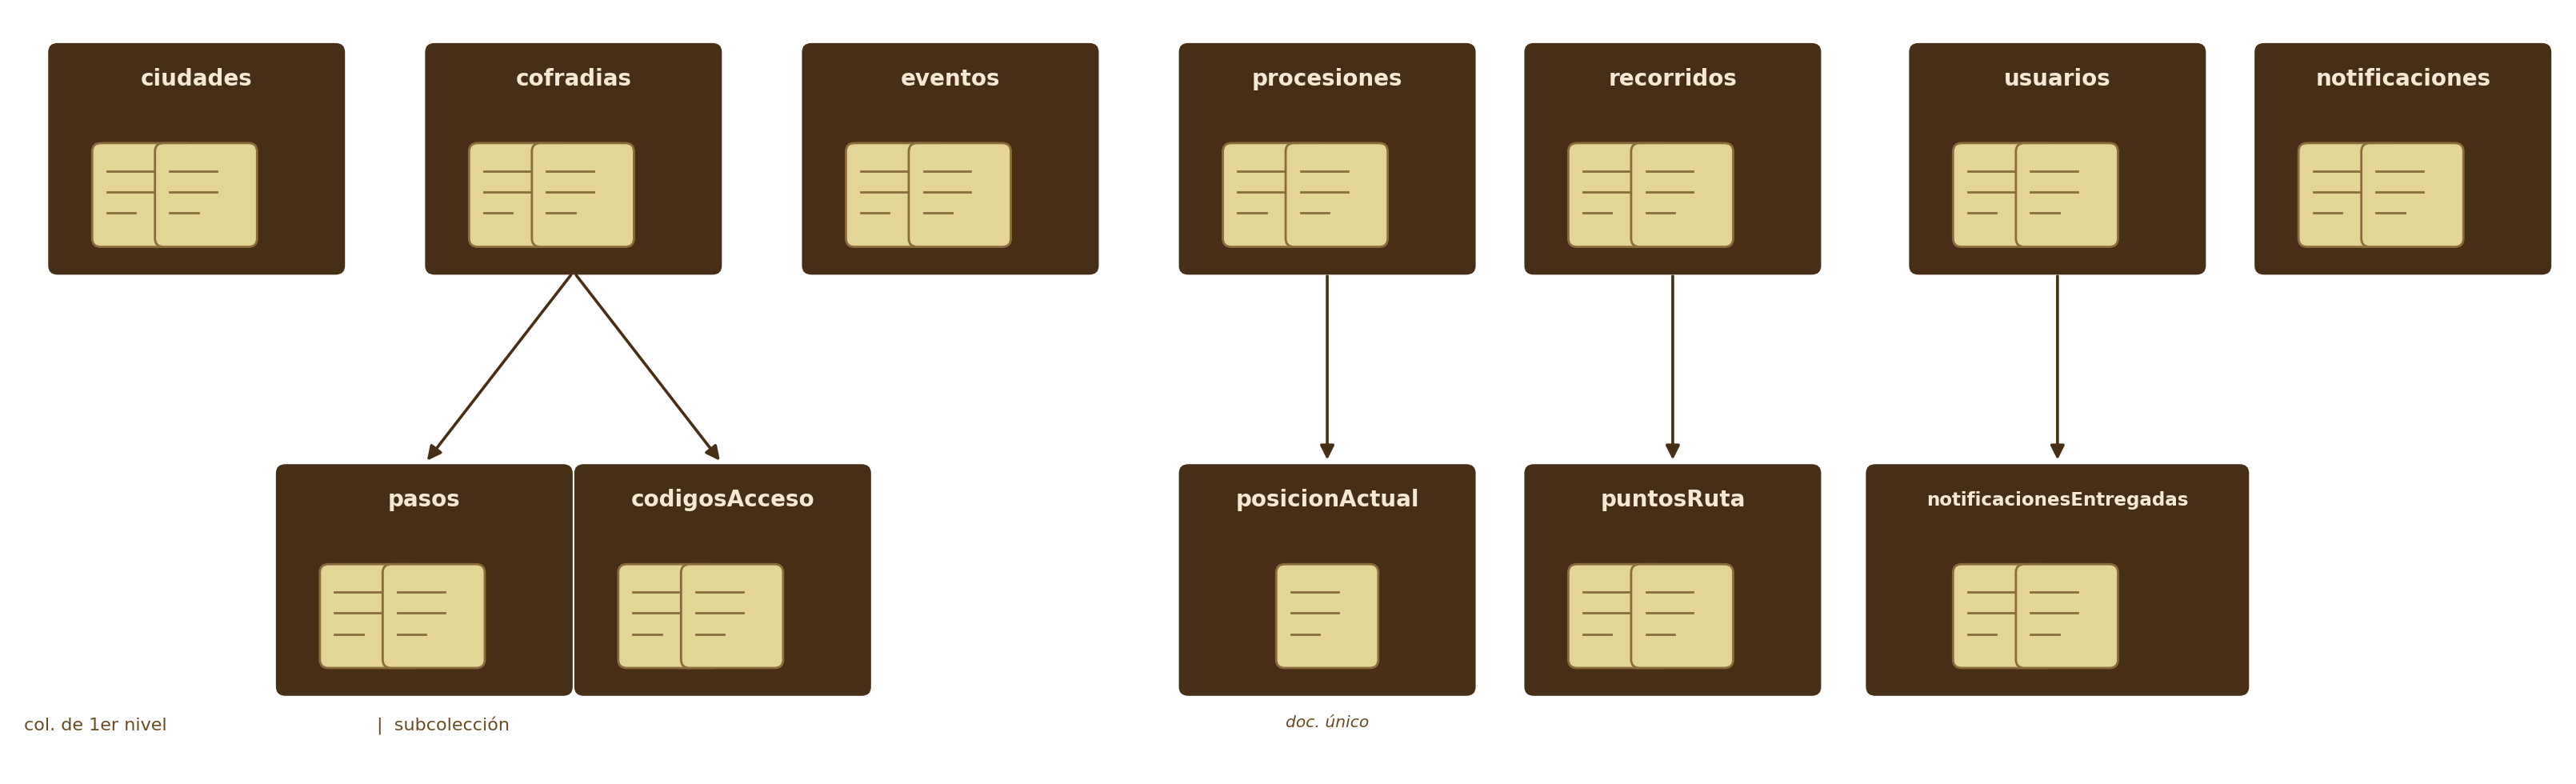
\includegraphics[width=0.9\textwidth]{imagenes/estructura_firestore.png}
    \caption{Estructura de colecciones y subcolecciones de Cloud Firestore}
    \label{fig:EstructuraFirestore}
\end{figure}

El Apéndice~\ref{cap:esquemaBD} recoge, a nivel de campo, el esquema completo de cada colección y subcolección --tipos de dato y referencias incluidas-- para quien necesite el detalle completo de la base de datos.

\subsubsection{Interfaces de usuario}
 
Paralelamente a las decisiones de arquitectura y de base de datos, se ha diseñado en Figma \cite{figma} el conjunto de pantallas del perfil de ciudadano mediante \emph{mockups}\footnote{Mockup: representación visual estática de la interfaz de una aplicación, sin funcionalidad real, utilizada para planificar el diseño antes de su implementación.}, que sirven de referencia visual para la implementación posterior. Se ha optado por diseñar de forma conjunta todas las pantallas del perfil ciudadano, aunque no todas se implementen en esta primera iteración, para garantizar una línea visual coherente desde el principio y evitar rediseños parciales más adelante. De ellas, en esta primera iteración se implementan únicamente la selección de ciudad, la pantalla de inicio y los listados y fichas de detalle de cofradías, procesiones, pasos y eventos; el resto se retoman en la iteración a la que corresponden: el mapa en vivo en la Iteración 2, el modo cofrade y la ubicación compartida del perfil en la Iteración 3, y el calendario, la búsqueda y las preferencias de notificaciones del perfil en iteraciones posteriores.
 
Todas las pantallas comparten una estética oscura con acentos dorados, que evoca la iluminación de cirios y el ambiente nocturno característico de las procesiones, y una barra de navegación inferior fija con cinco secciones (\emph{Inicio}, \emph{Calendario}, \emph{Mapa}, \emph{Buscar} y \emph{Perfil}), que se corresponde directamente con el paquete \texttt{navigation/} descrito en el apartado de arquitectura. Los listados de cofradías, procesiones, pasos y eventos ya no ocupan una sección propia de la barra de navegación, sino que se accede a ellos desde un menú contextual en la pantalla de \emph{Inicio}, tal y como se explica más adelante.
 
La paleta de color se apoya en tonos marrón muy oscuro, casi negro, para el fondo (\texttt{\#1E1008}, \texttt{\#120A06}, \texttt{\#34150E}, \texttt{\#472F17}), dorados como color de acento para títulos, iconos activos y elementos interactivos (\texttt{\#C9A84C}, \texttt{\#9A7D60}), tonos crema para tarjetas y textos secundarios (\texttt{\#F0E0C8}, \texttt{\#E3D595}) y blanco (\texttt{\#FFFFFF}) para el texto principal sobre fondo oscuro; un verde puntual (\texttt{\#37E37E}) se reserva para indicadores de estado, como una procesión en curso. En cuanto a la tipografía, se combinan tres familias: \textbf{Cormorant Garamond}, una serifa elegante, para los títulos, coherente con la estética evocada; \textbf{Lora}, también serifa pero más neutra, para el texto de lectura extensa (historia de una cofradía, descripción de un paso); y \textbf{Sora}, de palo seco, para los elementos de interfaz (botones, etiquetas, barra de navegación), donde interesa más la legibilidad a tamaños pequeños que el carácter estético. Estas decisiones se apoyan, además del criterio propio, en las pautas de \emph{Material Design~3} \cite{materialdesign3}, la guía de diseño de interfaz de Google, en particular en lo relativo al contraste de color, el tamaño mínimo táctil de los elementos interactivos y la estructura de la barra de navegación inferior.
 
\paragraph{Selección de ciudad}
 
Es la primera pantalla que ve cualquier usuario, ya que toda la información de la aplicación (cofradías, procesiones, eventos) está filtrada por la ciudad seleccionada, tal y como se refleja en la colección \texttt{ciudades} descrita en el apartado anterior. El usuario puede buscar su ciudad o elegirla de una lista con el número de procesiones disponibles en cada una.
 
\begin{figure}[H]
    \centering
    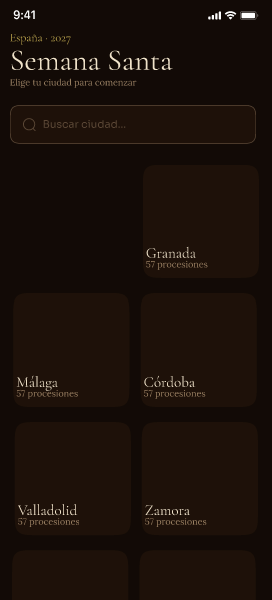
\includegraphics[width=0.45\textwidth]{imagenes/eleguirCiudad.png}
    \caption{Mockup de la pantalla de selección de ciudad}
    \label{fig:mockupCiudad}
\end{figure}
 
\paragraph{Inicio}
 
Muestra la información general del día de Semana Santa seleccionado: un aviso destacado si existe alguna incidencia relevante (por ejemplo, un retraso en el horario de salida), la procesión que está en curso en ese momento si la hay, unas estadísticas generales de la ciudad (número de cofradías, procesiones y nazarenos) y el listado de procesiones y eventos programados para el día, marcando cuáles son favoritos del ciudadano. Desde el menú contextual de esta pantalla (icono \emph{overflow} superior derecho) se accede, además, a los listados independientes de cofradías, procesiones, pasos y eventos.
 
\begin{figure}[H]
    \centering
    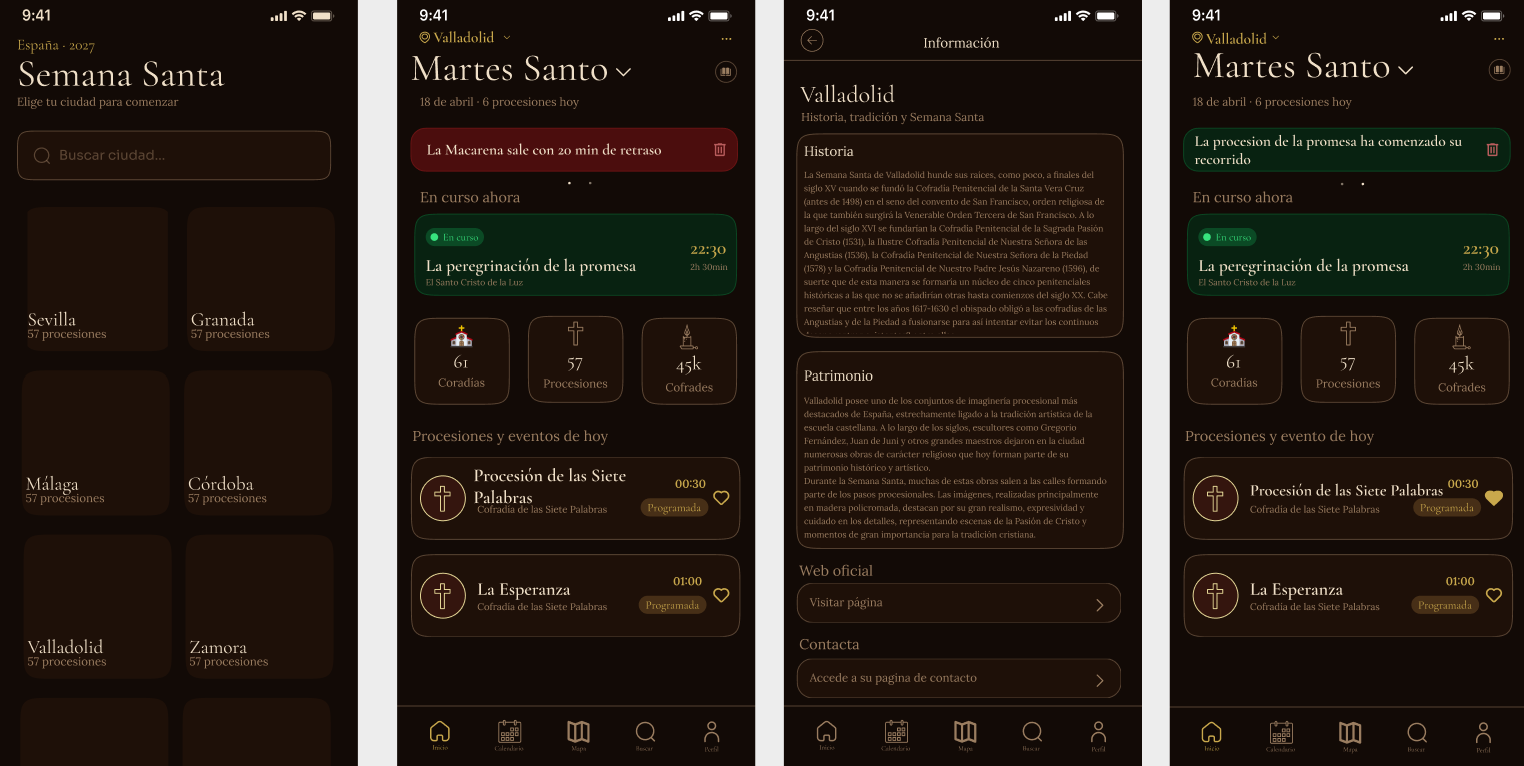
\includegraphics[width=0.9\textwidth]{imagenes/inicioYfav.png}
    \caption{Mockup de la pantalla de inicio: aviso de retraso, procesión en curso, estadísticas y agenda del día}
    \label{fig:mockupInicio}
\end{figure}
 
\paragraph{Calendario}
 
Complementa a la pantalla de inicio permitiendo consultar cualquier otro día de la Semana Santa, no solo el actual. Ofrece dos niveles de detalle: una vista mensual completa, con un indicador en los días que tienen procesiones programadas, y una vista semanal con la agenda del día seleccionado, listando sus procesiones con horario y duración.
 
\begin{figure}[H]
    \centering
    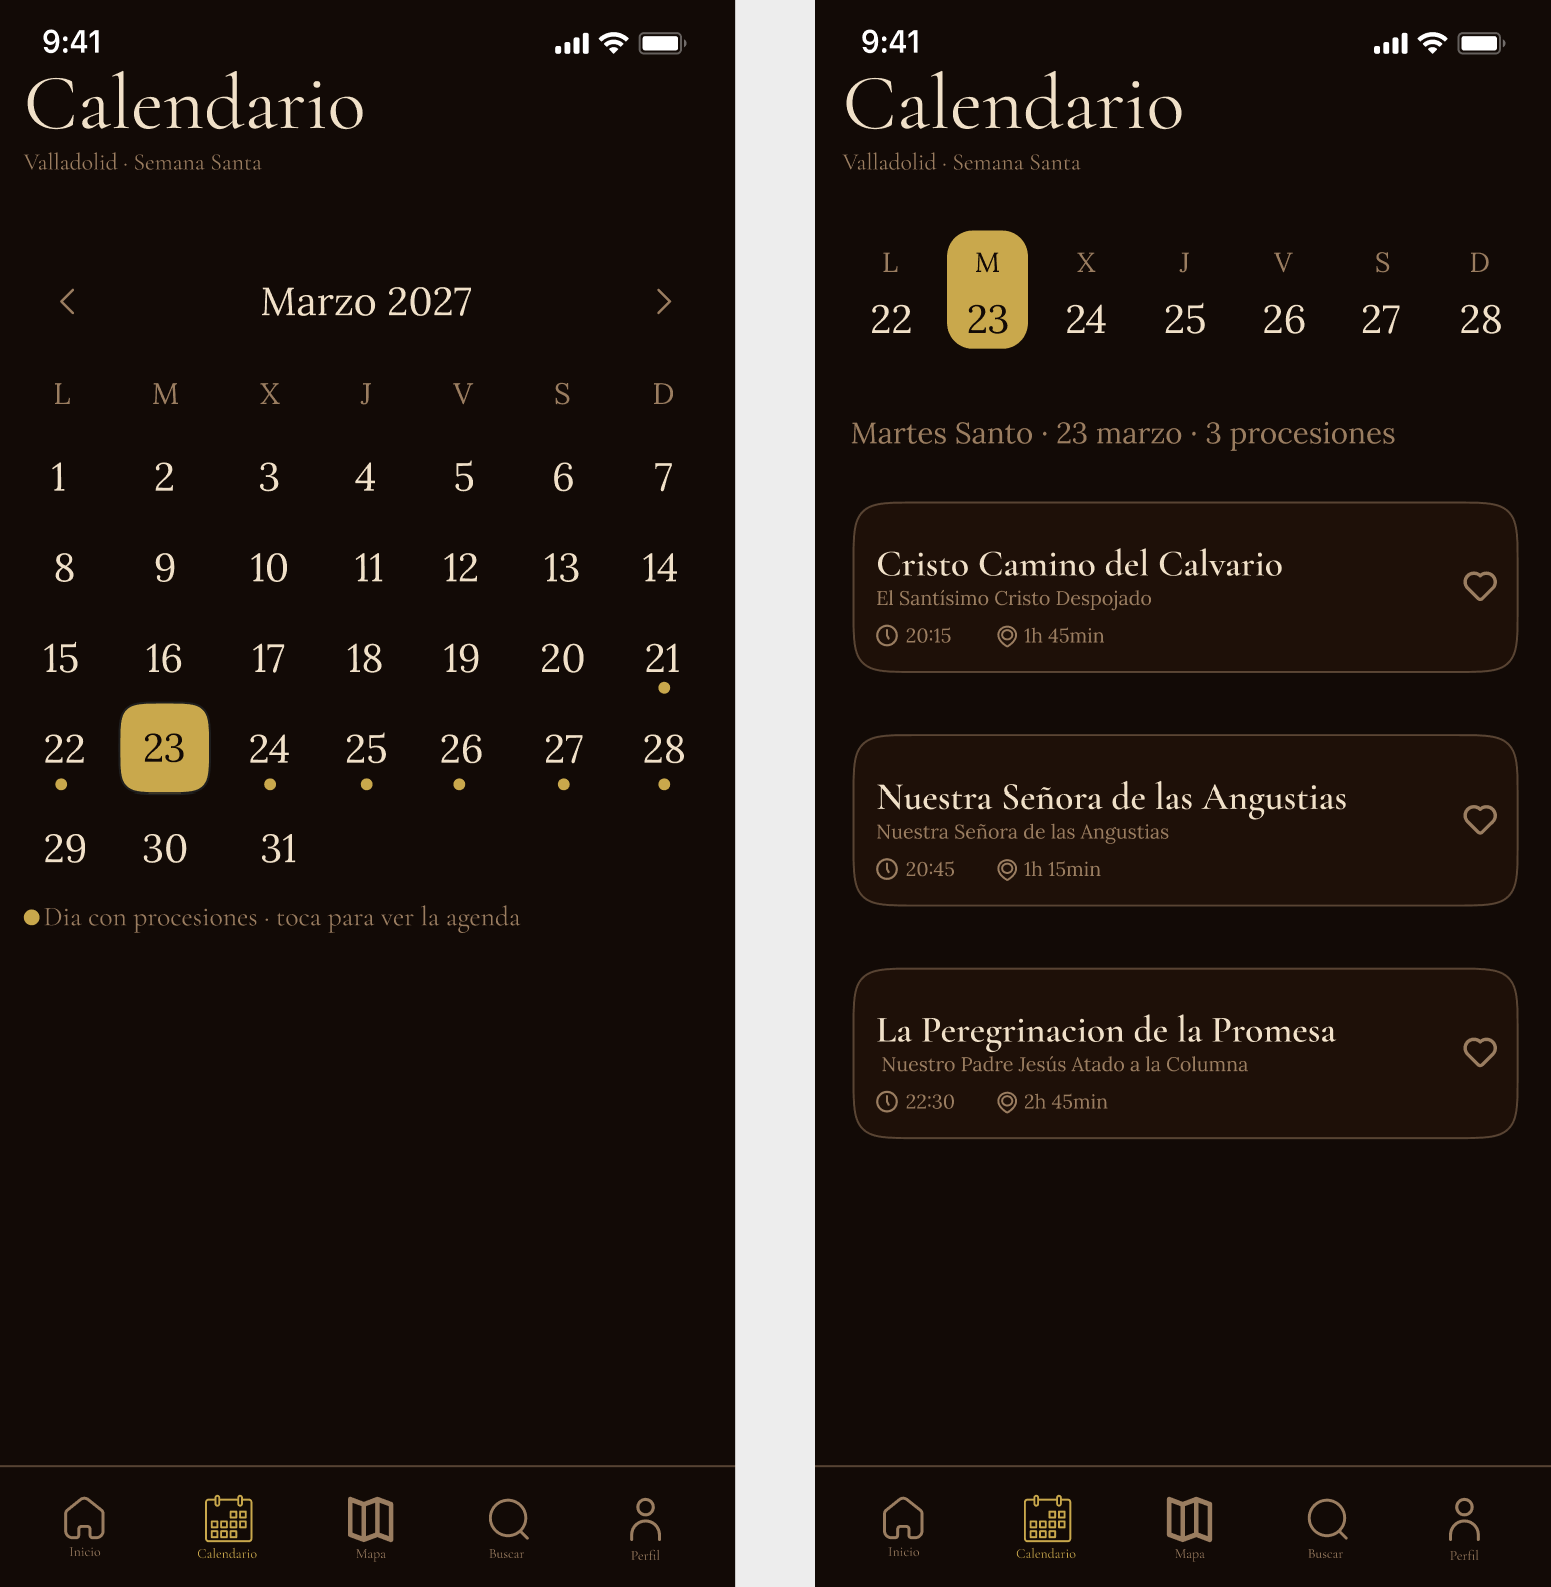
\includegraphics[width=0.9\textwidth]{imagenes/calendario.png}
    \caption{Mockup de la pantalla de calendario: vista mensual y agenda del día seleccionado}
    \label{fig:mockupCalendario}
\end{figure}
 
\paragraph{Listados de cofradías, procesiones, pasos y eventos}
 
Cada uno de estos cuatro elementos del dominio cuenta con su propio listado, accesible desde el menú de la pantalla de Inicio, con buscador propio y sin más información que el nombre de cada elemento, ya que su detalle se consulta accediendo a la ficha correspondiente.
 
\begin{figure}[H]
    \centering
    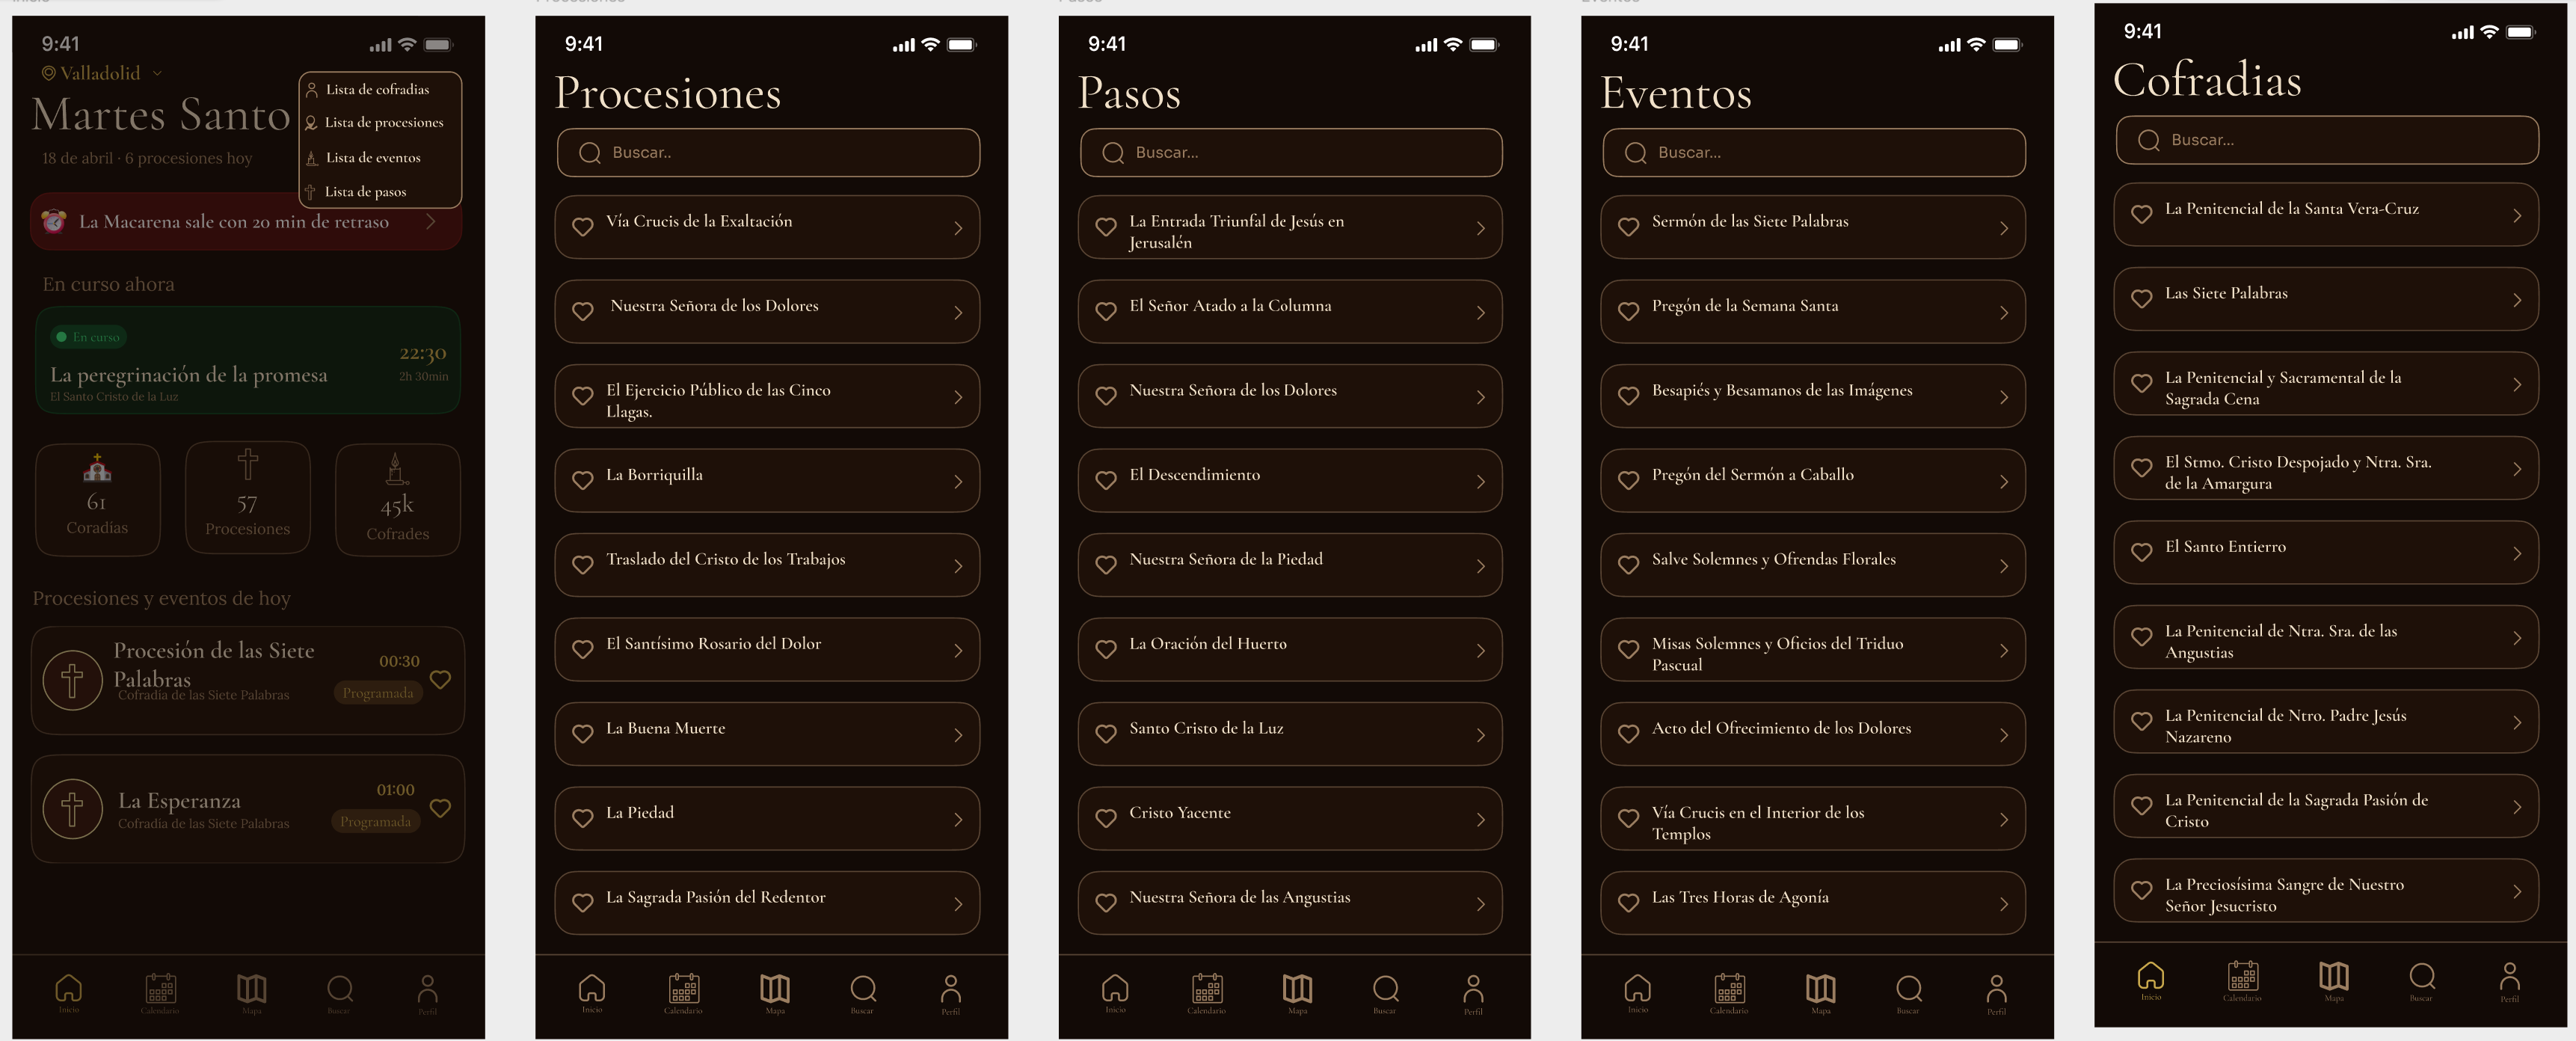
\includegraphics[width=0.95\textwidth]{imagenes/listados.png}
    \caption{Mockup del menú de la pantalla de inicio y de los listados de procesiones, pasos, eventos y cofradías}
    \label{fig:mockupListados}
\end{figure}
 
\paragraph{Detalle de cofradía y de paso}
 
La ficha de una cofradía muestra su historia, su web oficial, las procesiones y el evento que organiza y los pasos que la componen. De forma análoga, la ficha de un paso muestra una imagen, su historia y origen, un análisis artístico y su web oficial, siguiendo la misma estructura visual que la ficha de cofradía para mantener la coherencia del conjunto.
 
\begin{figure}[H]
    \centering
    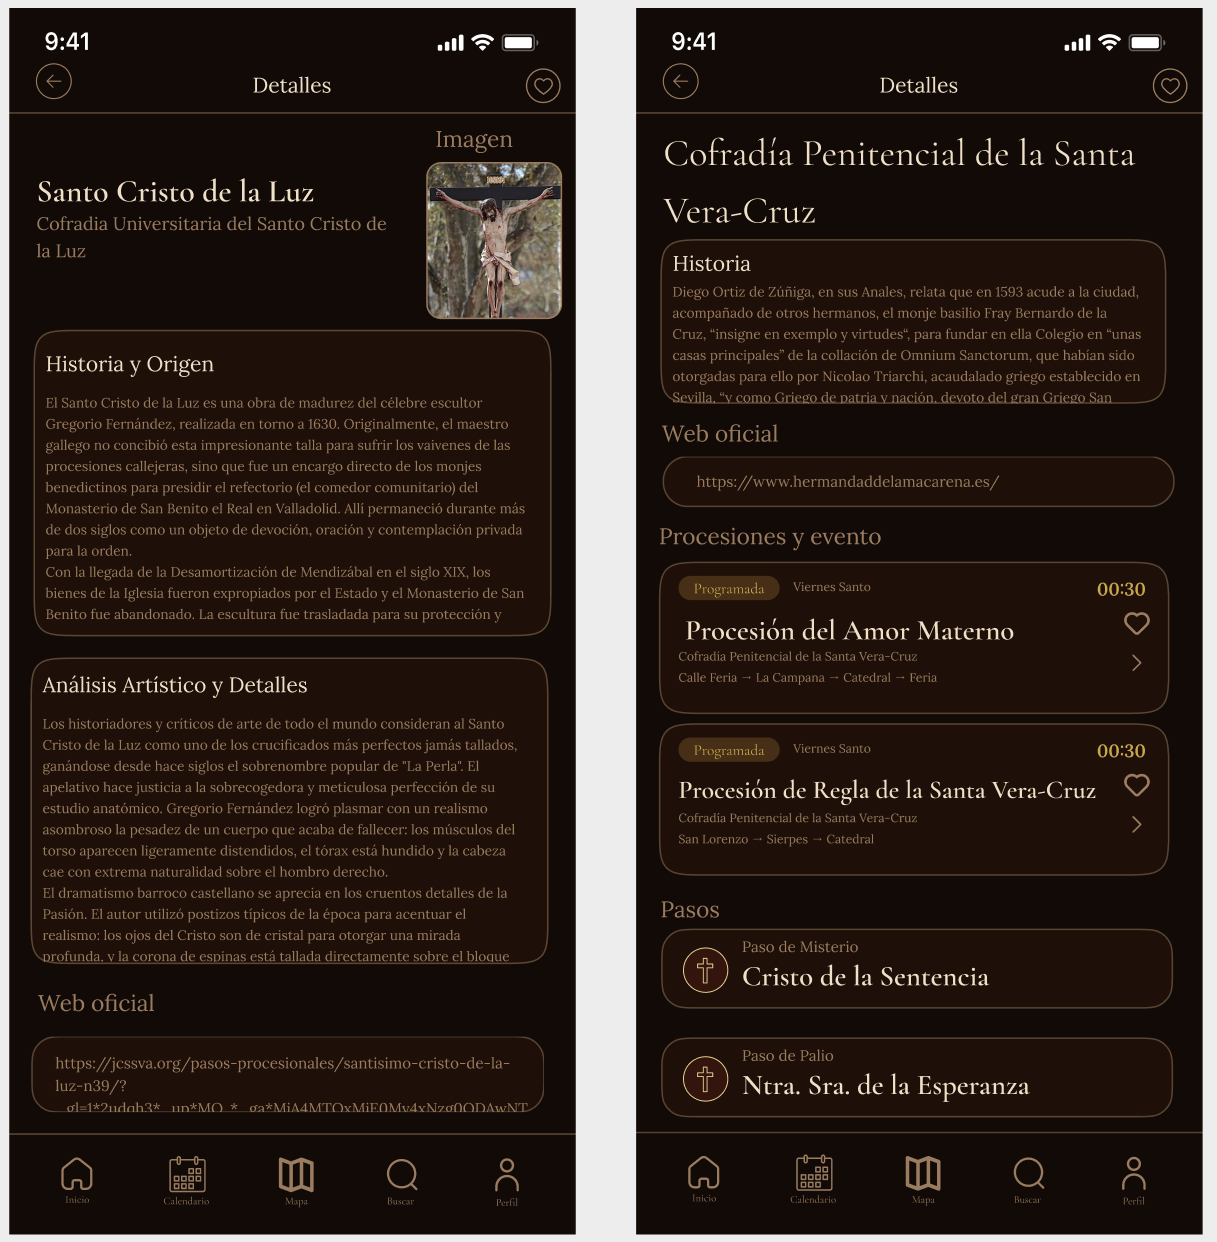
\includegraphics[width=0.9\textwidth]{imagenes/infoPasoyCofradia.png}
    \caption{Mockup del detalle de un paso y de una cofradía}
    \label{fig:mockupDetalleCofradiaPaso}
\end{figure}
 
\paragraph{Detalle de procesión}
 
Muestra el estado de la procesión (programada, en curso o finalizada), su día y hora de salida, duración, número de nazarenos, los pasos que participan en ella y su recorrido sobre un mapa, con un botón de acceso directo al mapa en vivo si la procesión está en curso. Además, de forma similar a la ficha de una cofradía, cada procesión tiene una pantalla de información ampliada con la historia y el origen del desfile.
 
\begin{figure}[H]
    \centering
    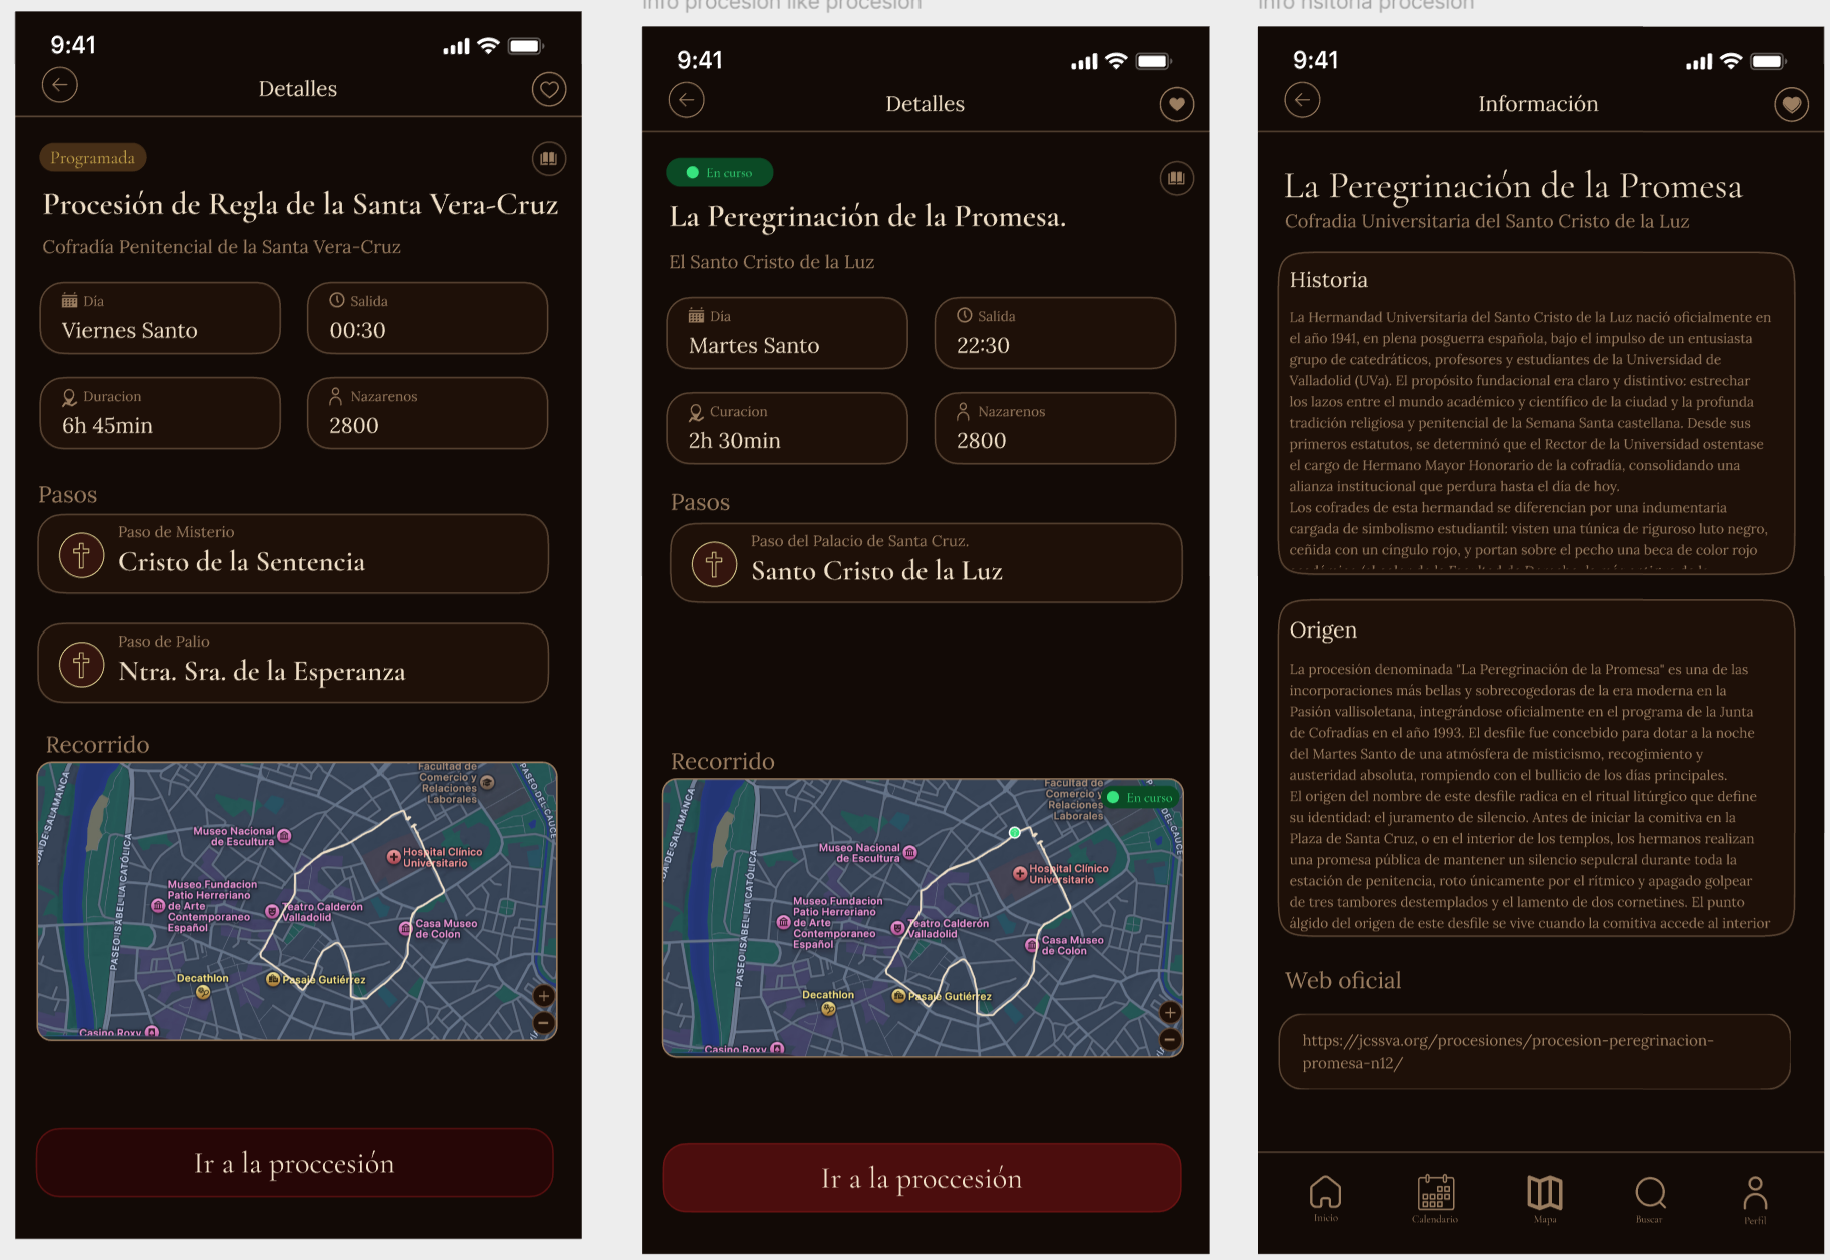
\includegraphics[width=0.95\textwidth]{imagenes/procesionDetalleNuevo.png}
    \caption{Mockup del detalle de una procesión (programada y en curso) y de su información ampliada}
    \label{fig:mockupDetalleProcesion}
\end{figure}
 
\paragraph{Buscar}
 
Permite localizar procesiones, pasos y eventos combinando texto libre con filtros por día de Semana Santa y por estado (programada, en curso o finalizada), mostrando un mensaje cuando ningún resultado cumple los filtros seleccionados. Su funcionalidad se implementa en una iteración posterior.
 
\begin{figure}[H]
    \centering
    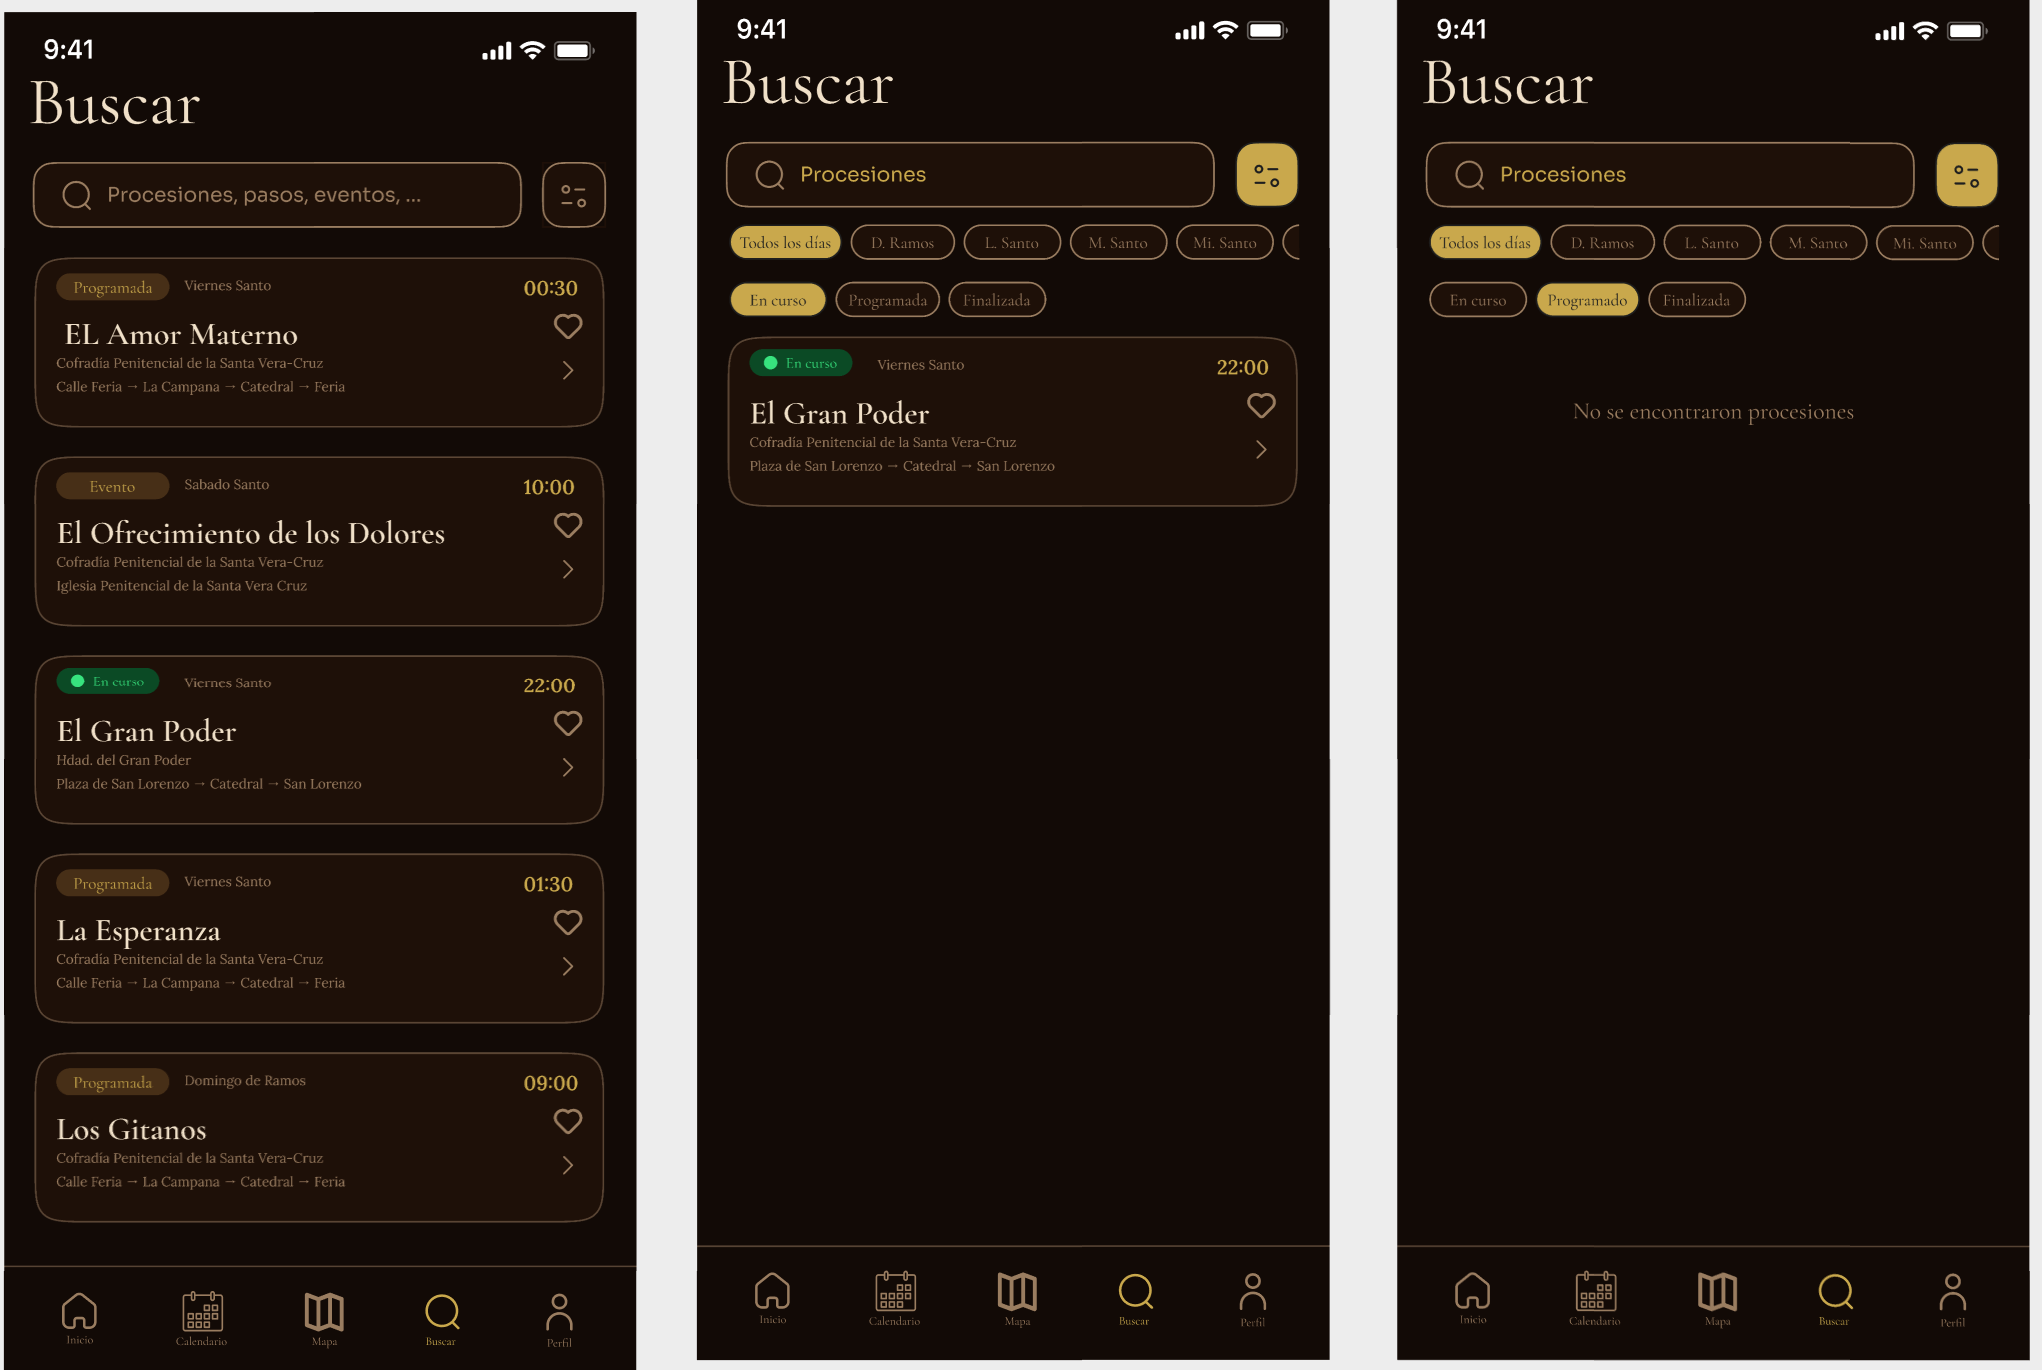
\includegraphics[width=0.9\textwidth]{imagenes/buscaryFiltrar.png}
    \caption{Mockup de la pantalla de búsqueda con filtros por día y estado}
    \label{fig:mockupBuscar}
\end{figure}
 
\paragraph{Mapa en Vivo}
 
Mostrará sobre un mapa de Google Maps la posición en tiempo real de las procesiones en curso y la ubicación del propio ciudadano, junto con un listado de las procesiones actualmente en movimiento desde el que centrar el mapa sobre una de ellas. Se implementa en la Iteración 2.
 
\begin{figure}[H]
    \centering
    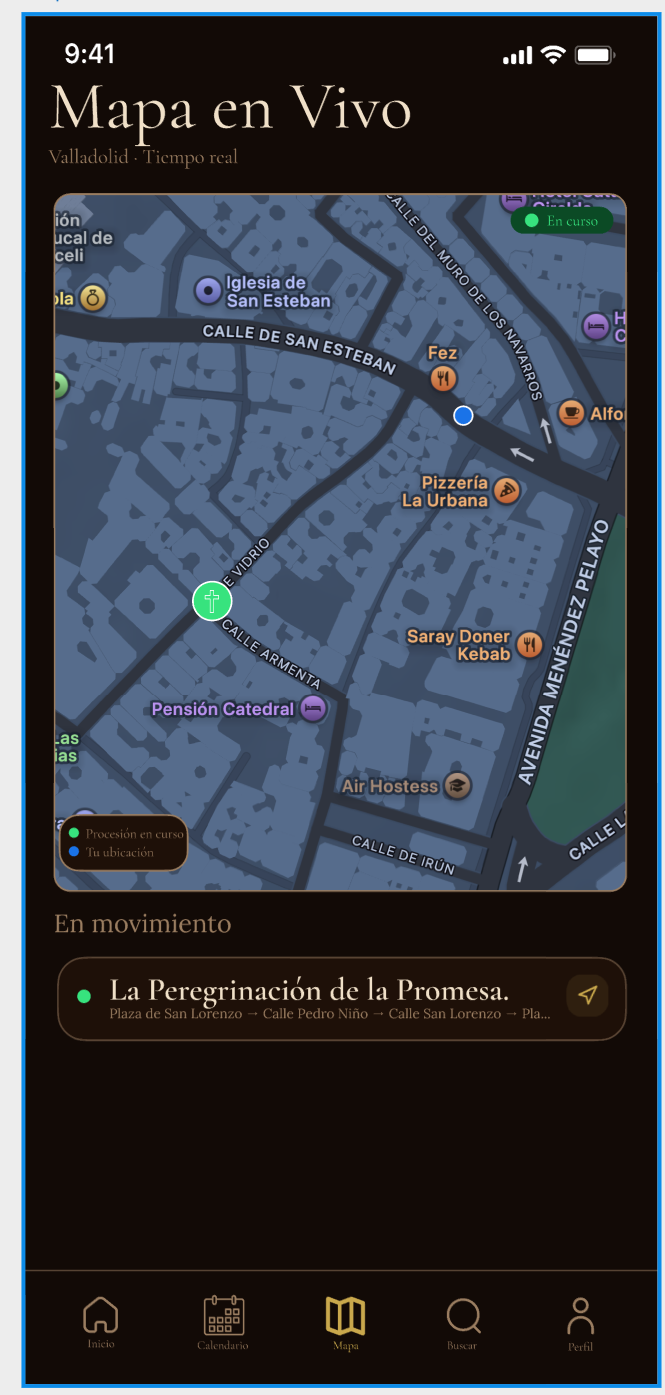
\includegraphics[width=0.45\textwidth]{imagenes/mapaEnVivo.png}
    \caption{Mockup del mapa en vivo}
    \label{fig:mockupMapa}
\end{figure}
 
\paragraph{Perfil}
 
Reúne la ciudad seleccionada y las cofradías/procesiones favoritas del ciudadano, el cambio entre el modo ciudadano y el modo cofrade, y las preferencias de notificaciones (avisos de procesiones en curso, alertas de tráfico y retrasos). En modo cofrade se añade además el botón para activar la ubicación compartida durante una procesión. El cambio de modo y la ubicación compartida se implementan en la Iteración 3; las preferencias de notificaciones, en una iteración posterior.
 
\begin{figure}[H]
    \centering
    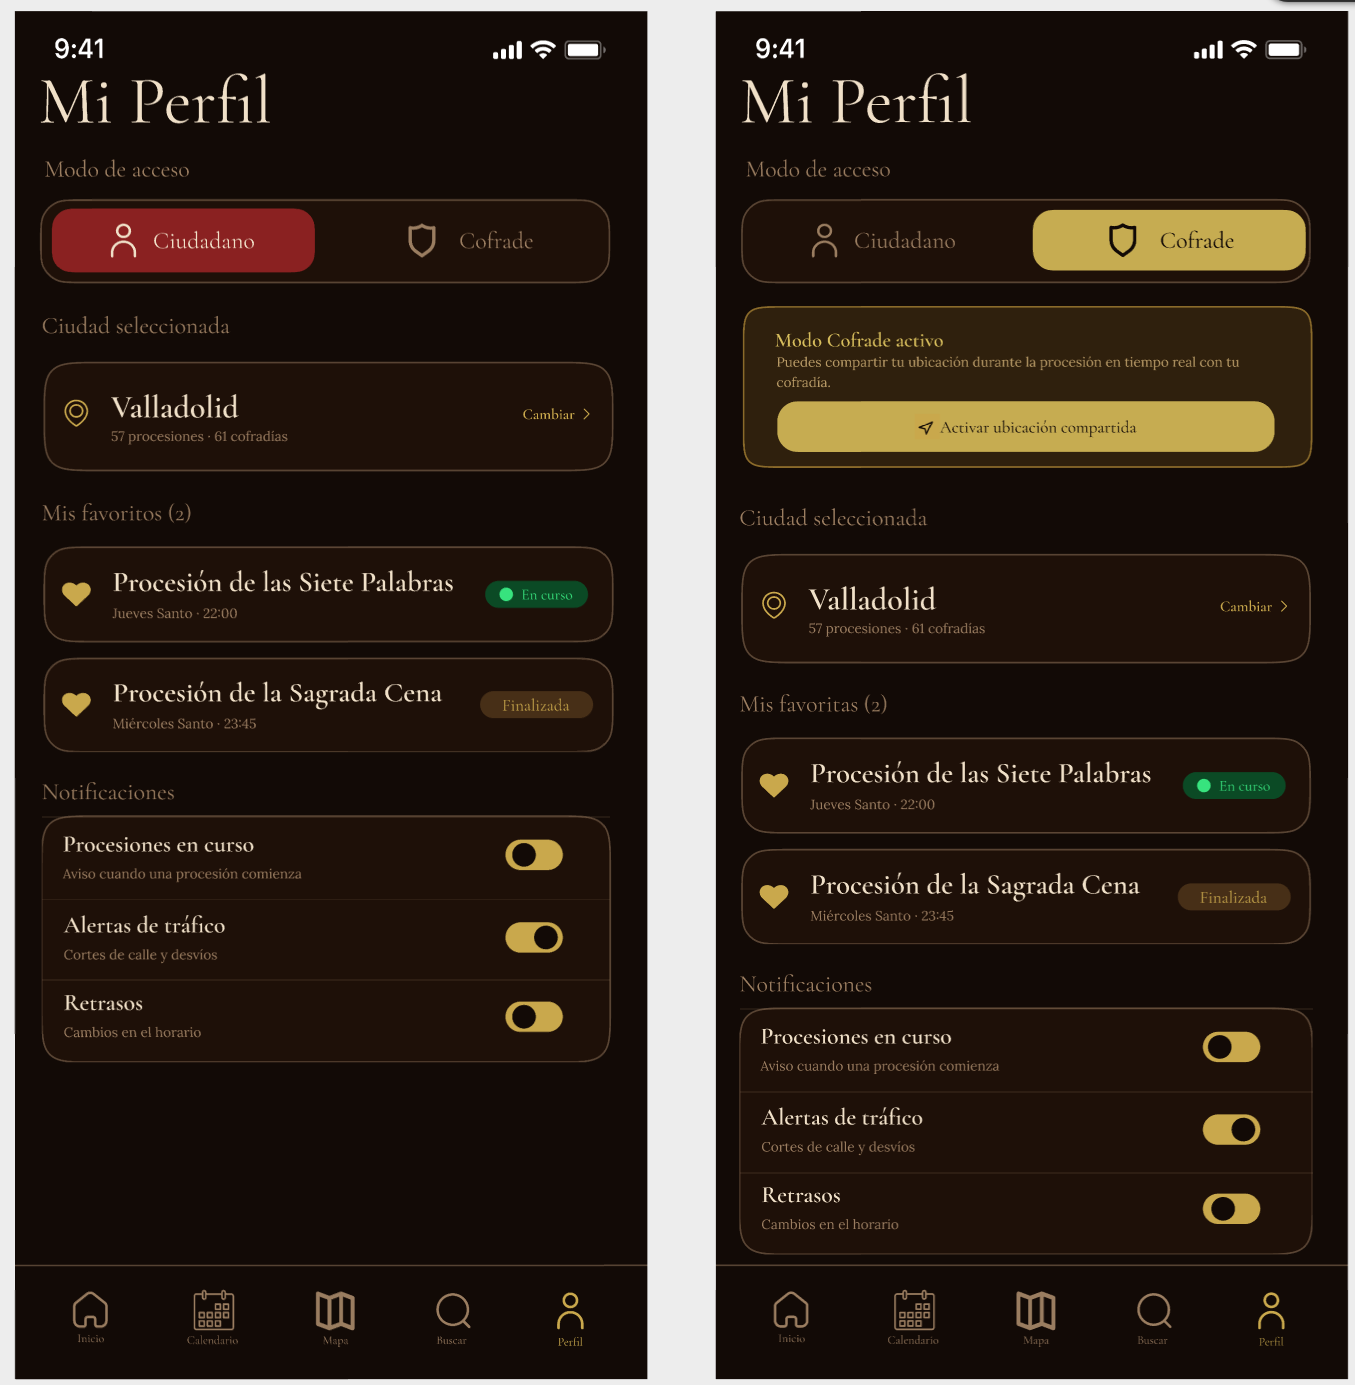
\includegraphics[width=0.9\textwidth]{imagenes/perfiles.png}
    \caption{Mockup de la pantalla de perfil, en modo ciudadano y en modo cofrade}
    \label{fig:mockupPerfil}
\end{figure}
 
\subsubsection{Patrones de diseño}
 
Un patrón de diseño \cite{larman2004} es una solución ya conocida y reutilizable a un problema que se repite con frecuencia en el desarrollo de software; su uso facilita la legibilidad, el mantenimiento y la escalabilidad del código. Para seleccionar los patrones aplicables a este proyecto se han revisado dos TFG previos de la escuela con una arquitectura similar (aplicación móvil apoyada en Firebase), de los que se han descartado los patrones \emph{Builder} y \emph{Abstract Factory}: en Java se justifican porque los constructores de clases no admiten bien parámetros opcionales, pero en JavaScript/TypeScript un objeto literal con esos mismos campos opcionales ya resuelve el mismo problema de forma nativa, y en ningún punto del sistema es necesario intercambiar familias completas de implementaciones. Los siete patrones finalmente aplicados son los siguientes:
 
\begin{itemize}
    \item \textbf{Singleton}: patrón que garantiza que una clase tenga una única instancia en toda la aplicación y un punto de acceso global a ella, evitando crear varias copias innecesarias. En este proyecto, la inicialización del SDK de Firebase (\texttt{firebase/config}) se realiza una única vez y esa misma instancia se reutiliza en el resto de la aplicación.
    \item \textbf{Repository}: patrón que separa la lógica de acceso a los datos del resto de la aplicación, ocultando los detalles de cómo y dónde se almacenan. La capa \texttt{services} es la única parte del código que conoce el SDK de Firebase; el resto de la aplicación solo invoca funciones como \texttt{procesionService.} \texttt{obtenerActivas(ciudadId)}, sin saber que por detrás se está consultando Firestore. Esto facilitaría cambiar de proveedor de backend en el futuro (línea de trabajo futuro, Sección~\ref{cap:trabajo_futuro}) sin modificar ninguna pantalla.
    \item \textbf{Observer}: patrón en el que uno o varios elementos (``observadores'') se suscriben a los cambios de otro elemento y son notificados automáticamente cuando este cambia, en lugar de tener que preguntar repetidamente. Los \emph{listeners} de Firestore (\texttt{onSnapshot}) funcionan así: notifican a la interfaz cada vez que cambia la posición de una procesión o llega una notificación nueva.
    \item \textbf{Factory Method}: patrón que centraliza en una única función la creación de un objeto, delegando en ella la decisión de qué variante concreta construir. El dominio distingue \texttt{Aviso} y \texttt{Alerta} como subtipos de \texttt{Notificacion} (Figura~\ref{fig:DiagramDomain}); una función fábrica construye el objeto correcto según los campos \texttt{tipoAlerta} y \texttt{fechaExpiracion} antes de guardarlo en Firestore.
    \item \textbf{Context/Provider}: convención propia de React (no un patrón GoF\footnote{GoF (\emph{Gang of Four}): apodo con el que se conoce a los cuatro autores del libro \emph{Design Patterns} \cite{gof} (1994), que popularizó el catálogo clásico de patrones de diseño orientado a objetos (Singleton, Observer, Factory Method, entre otros).} clásico) que permite exponer un dato o estado a cualquier pantalla de la aplicación sin tener que pasarlo manualmente de componente en componente. \texttt{AuthContext} y \texttt{LocationContext} exponen así el usuario autenticado y los permisos de ubicación a cualquier pantalla que los necesite.
    \item \textbf{Facade}: patrón que ofrece una única función sencilla como punto de entrada a una operación que, por detrás, involucra varios pasos o subsistemas distintos. El caso de uso ``Compartir ubicación durante procesión'' (RF-15) esconde tras la llamada \texttt{geoService.iniciarCompartirUbicacion} \texttt{(procesionId)} la solicitud de permiso de GPS, la escritura periódica en Firestore y la gestión de una posible pérdida de conexión.
    \item \textbf{Adapter}: patrón que convierte el formato de datos de un sistema externo al formato interno que espera la aplicación, permitiendo que ambos ``encajen'' sin modificar ninguno de los dos. Las notificaciones \emph{push} de Firebase Cloud Messaging llegan con un formato plano (título, cuerpo, y un mapa de texto), distinto del modelo interno tipado \texttt{Alerta}/\texttt{Aviso}; una función adaptadora convierte ese \emph{payload} recibido al modelo de dominio antes de utilizarlo en la aplicación.
\end{itemize}
 
\subsection{Implementacion}
 
\subsection{Pruebas}
\section{2ª Iteración}\label{cap:2_iteracion}

\subsection{Analisís}

\subsection{Diseño}

\subsection{Implementacion}

Esta segunda iteración implementa en el backend las entidades necesarias para el sistema de mapas: \texttt{Recorrido}, \texttt{Ubicacion} y \texttt{PuntoRuta}, siguiendo la misma estructura de cuatro capas ya establecida en la Iteración 1 y documentada a nivel de campo en el Apéndice~\ref{cap:esquemaBD}.

\texttt{Ubicacion} es una tabla nueva, sin equivalente directo en el modelo de dominio original (Figura~\ref{fig:DiagramDomain}): agrupa en un único lugar la latitud, la longitud y la dirección que necesitan tanto \texttt{Evento} como \texttt{PuntoRuta}, para poder reutilizar el mismo punto geográfico desde varias entidades sin duplicar datos --por ejemplo, la sede de una cofradía y un punto de interés del recorrido que coincidan en el mismo templo--.

\texttt{PuntoRuta} es, además, la raíz de una jerarquía de herencia real de tablas (estrategia \texttt{JOINED} de JPA): un punto ``de paso'' simple se guarda directamente en \texttt{puntos\_ruta}, mientras que un punto ``de interés'', con nombre, descripción, imagen y una categoría, extiende esa tabla en \texttt{PuntoDeInteres}. Durante esta implementación se detectó, además, que un mismo punto de ruta puede formar parte de \textbf{varios} recorridos --varias procesiones pueden compartir un mismo tramo de calle--, así que la relación entre \texttt{Recorrido} y \texttt{PuntoRuta} se resolvió como una relación N:M mediante la tabla intermedia \texttt{recorrido\_puntos\_ruta}, que además guarda el orden del punto y su hora prevista de paso \emph{en ese recorrido concreto}, ya que un mismo punto puede ocupar posiciones y horas distintas según el recorrido del que forme parte.

\subsection{Pruebas}

Al igual que en la Iteración 1, la verificación de estas entidades se ha realizado de forma manual mediante la documentación interactiva de springdoc-openapi (\texttt{/swagger-ui.html}). La batería de pruebas automatizadas queda pendiente y se documentará en el Capítulo~\ref{cap:pruebas}.

\section{3ª Iteración}\label{cap:3_iteracion}

\subsection{Analisís}

\subsection{Diseño}

\subsection{Implementacion}

Esta tercera iteración implementa la geolocalización en tiempo real y el perfil de cofrade, lo que exige dos piezas que hasta ahora no hacían falta: la entidad \texttt{Procesion} propiamente dicha y, por primera vez en el proyecto, un mecanismo de autenticación --hasta este punto todos los \emph{endpoints} eran de lectura o gestión pública, ya que el ciudadano nunca se registra (RI-01)--.

\texttt{Procesion} se implementa como una extensión real de \texttt{Evento} (herencia con estrategia \texttt{JOINED} de JPA, Apéndice~\ref{cap:esquemaBD}) en lugar de una simple referencia: hereda nombre, historia, fecha, estado, ubicación y cofradías participantes de \texttt{Evento}, y añade únicamente su fecha de inicio y fin y su \texttt{Recorrido} asociado (relación 1:1, opcional --una procesión puede programarse antes de tener ruta definida--).

Para el acceso como cofrade (caso de uso ``Acceso como cofrade'', Sección~\ref{cap:modeloInteraccion}) se implementa \texttt{CodigoAcceso} junto con la infraestructura de autenticación: tokens \textbf{JWT} generados y validados con la biblioteca \texttt{jjwt}, un filtro de Spring Security que intercepta cada petición para comprobar el token, y el \emph{endpoint} \texttt{POST /auth/codigo-acceso}, que valida el código y devuelve directamente un token identificado con la cofradía correspondiente, sin registrar ninguna fila de usuario (Apéndice~\ref{cap:esquemaBD}, Sección~\ref{sec:usuariosBD}). La clase \texttt{Cofrade} del modelo de dominio (Figura~\ref{fig:DiagramDomain}) se implementa así como una representación construida en memoria a partir de ese token en cada petición, no como una entidad persistida.

Por último, se implementa la funcionalidad de compartir ubicación (RF-15) mediante el \emph{endpoint} \texttt{POST /procesiones/\{id\}/posiciones}, que registra cada actualización de posición del cofrade como una lectura --o \emph{ping}-- anónima en \texttt{PosicionActual}, y \texttt{GET /procesiones/\{id\}/ubicacion}, que calcula la posición agregada de la procesión en ese momento como el promedio de los \emph{pings} recibidos en los últimos 60 segundos, cubriendo así el requisito RNF-08.

\subsection{Pruebas}

Al igual que en las iteraciones anteriores, la verificación se ha realizado de forma manual mediante springdoc-openapi (\texttt{/swagger-ui.html}), incluyendo la obtención de un token válido con \texttt{POST /auth/codigo-acceso} y su uso en las peticiones protegidas subsiguientes. La batería de pruebas automatizadas queda pendiente y se documentará en el Capítulo~\ref{cap:pruebas}.

\section{4ª Iteración}\label{cap:4_iteracion}

\subsection{Analisís}

\subsection{Diseño}

\subsection{Implementacion}

Esta cuarta iteración implementa el panel de la Junta de Cofradías: el acceso mediante credenciales propias y el mecanismo de control de acceso que restringe, entidad por entidad, qué puede gestionar cada Junta.

Se implementa \texttt{MiembroJuntaCofradia} --persona con credenciales que pertenece a la Junta de una ciudad, pudiendo haber varios miembros por Junta-- y el \emph{endpoint} \texttt{POST /auth/login}, que compara el \texttt{email} y la contraseña (\emph{hash} BCrypt) recibidos y devuelve un token JWT con el identificador del miembro y su rol, siguiendo el mismo mecanismo de autenticación introducido en la Iteración 3.

Sobre esa autenticación se implementa la autorización por rol que exige el requisito RNF-05: en la capa \texttt{Service} de cada entidad de contenido --\texttt{Cofradia}, \texttt{Paso}, \texttt{Evento}, \texttt{Procesion} y \texttt{CodigoAcceso}--, las operaciones de creación, edición y eliminación comprueban que quien las solicita es un miembro de la Junta que gestiona la ciudad a la que pertenece esa cofradía, antes de permitir la operación; en caso contrario, la API responde con un código \texttt{403} (prohibido). Esta comprobación se centraliza en un único método reutilizable en lugar de repetirse en cada entidad, para evitar duplicar la misma lógica de autorización varias veces. Las entidades \texttt{Recorrido}, \texttt{Ubicacion}, \texttt{PuntoRuta} y \texttt{PuntoDeInteres}, al no pertenecer a una única cofradía --se diseñaron como recursos reutilizables entre procesiones e incluso entre ciudades distintas, Sección~\ref{cap:2_iteracion}--, solo exigen que quien las gestione sea una Junta de Cofradías cualquiera, sin comparar ciudad.

\subsection{Pruebas}

Al igual que en las iteraciones anteriores, la verificación se ha realizado de forma manual: obtención de un token con \texttt{POST /auth/login} y comprobación de que las operaciones de gestión se aceptan o se rechazan (\texttt{403}) según la ciudad que gestiona cada Junta de prueba. La batería de pruebas automatizadas queda pendiente y se documentará en el Capítulo~\ref{cap:pruebas}.

\clearpage
%\chapter{Tecnologías utilizadas}\label{cap:tecnologias}
 
Este capítulo recoge, a modo de referencia, el conjunto de tecnologías, herramientas y servicios empleados en el desarrollo del proyecto, agrupados por la parte del sistema a la que pertenecen. La justificación de cada decisión --por qué esta tecnología y no otra-- se desarrolla con más detalle en el apartado \nameref{sec:decisionesTecnologicas} (Sección~\ref{cap:1_iteracion}); este capítulo se centra en describir brevemente cada pieza y su papel dentro del sistema.
 
\section{Cliente móvil}
 
\begin{itemize}
    \item \textbf{React Native} \cite{reactnative}: \emph{framework}\footnote{Framework: conjunto de herramientas y bibliotecas de código que facilitan el desarrollo de un tipo concreto de aplicación, proporcionando una estructura base sobre la que trabajar.} de Meta que permite escribir una única aplicación en JavaScript/TypeScript y ejecutarla tanto en Android como en iOS.
    \item \textbf{Expo} \cite{expo}: conjunto de herramientas sobre React Native recomendado por la documentación oficial de este último \cite{reactnative} para construir el código de la aplicación, en lugar de configurar manualmente el entorno nativo de cada plataforma. Aporta una biblioteca estándar de módulos nativos, un proceso de compilación gestionado (\emph{EAS Build}) y la publicación de actualizaciones del código sin pasar por las tiendas de aplicaciones.
    \item \textbf{react-native-maps} y \textbf{expo-location}: librerías utilizadas para la integración del mapa y el acceso a la geolocalización del dispositivo, respectivamente; esta última forma parte de la biblioteca estándar de Expo.
    \item \textbf{TanStack Query} \cite{reactquery}: librería de gestión de estado remoto que se encarga de las peticiones a la API propia (caché en memoria y en disco, reintentos automáticos y actualización periódica de los datos), utilizada para cubrir la disponibilidad sin conexión de los datos estáticos (RNF-03), tal y como se explica en la Sección~\ref{cap:1_iteracion}.
\end{itemize}
 
\section{Backend propio}
 
\begin{itemize}
    \item \textbf{Spring Boot} \cite{springboot}: \emph{framework} de Java sobre el que se construye la API REST\footnote{API REST: forma habitual de comunicación entre un cliente y un servidor propio, en la que el cliente pide o envía datos a través de peticiones HTTP a unas direcciones (\emph{endpoints}) definidas por el propio equipo de desarrollo.} del proyecto, siguiendo una arquitectura en capas (controlador, servicio, repositorio) descrita en la Sección~\ref{cap:1_iteracion}.
    \item \textbf{Spring Security} \cite{springsecurity} y \textbf{JWT} (\emph{JSON Web Token}) \cite{jwt}: mecanismo de autenticación y autorización de la API. Tras validar sus credenciales, el usuario recibe un token firmado que debe incluir en cada petición posterior; el servidor lo valida y comprueba el rol asociado antes de permitir el acceso a un recurso, sin necesidad de mantener sesión en el servidor.
    \item \textbf{Spring Data JPA} \cite{springdatajpa} e \textbf{Hibernate} \cite{hibernate}: capa de persistencia (\emph{Object-Relational Mapping} u ORM\footnote{ORM: técnica que traduce automáticamente entre los objetos de un lenguaje de programación orientado a objetos (Java, en este caso) y las tablas de una base de datos relacional, evitando escribir manualmente la mayoría de las sentencias SQL.}) que traduce las entidades Java del dominio a tablas de PostgreSQL y viceversa.
    \item \textbf{springdoc-openapi} \cite{springdoc}, basado en la especificación \textbf{OpenAPI} \cite{openapi}: genera automáticamente la documentación interactiva de la API a partir del propio código.
\end{itemize}
 
\section{Base de datos}
 
\begin{itemize}
    \item \textbf{PostgreSQL} \cite{postgresql}: sistema gestor de bases de datos relacional utilizado para almacenar toda la información persistente del sistema (ciudades, cofradías, procesiones, recorridos, usuarios, notificaciones, etc.). El esquema completo se detalla en el Apéndice~\ref{cap:esquemaBD}.
\end{itemize}
 
\section{Servicios externos}
 
\begin{itemize}
    \item \textbf{Expo Push Notifications} \cite{expo}: servicio de notificaciones \emph{push} de la propia plataforma Expo (\texttt{exp.host}), en lugar de Firebase Cloud Messaging. El backend propio es quien decide cuándo se envía una notificación (por ejemplo, cuando una Junta de Cofradías crea una notificación de cambio de horario o cancelación) y se la manda a Expo mediante una petición HTTP corriente a su API; es Expo quien por detrás entrega esa notificación al dispositivo del usuario a través de FCM (Android) o de APNs (iOS), sin que el backend propio tenga que integrarse directamente con ninguno de los dos ni gestionar credenciales de Firebase o de Apple. Se ha optado por esta vía en lugar del Firebase Admin SDK planteado inicialmente porque, al usar ya Expo como plataforma del cliente móvil, evita añadir un segundo proveedor de \emph{push} y sus credenciales propias al proyecto.
    \item \textbf{Google Maps Platform} \cite{googlemapsapi}: visualización de mapas y cálculo de rutas en el cliente, ya justificado en el estado de la cuestión (Sección~1.3.2).
\end{itemize}
 
\section{Despliegue y alojamiento}
 
\begin{itemize}
    \item \textbf{Railway} \cite{railway}: plataforma \emph{PaaS} (\emph{Platform as a Service}) utilizada para alojar tanto la API de Spring Boot como la base de datos PostgreSQL. Se ha elegido frente a un servidor propio (VPS) porque simplifica el despliegue continuo desde GitHub, no requiere gestionar manualmente el sistema operativo del servidor y dispone de un plan gratuito suficiente para las necesidades del proyecto durante el desarrollo del TFG \cite{railwaypricing}, en línea con el planteamiento de \nameref{sec:decisionesTecnologicas} de priorizar el tiempo de desarrollo dado que el proyecto lo lleva a cabo una única persona. El manual de despliegue completo se recoge en el Apéndice~\ref{cap:manual_despliegue}.
\end{itemize}
 
\section{Herramientas de desarrollo}
 
\begin{itemize}
    \item \textbf{Android Studio} \cite{androidstudio} y \textbf{Visual Studio Code} \cite{vscode}: entornos de desarrollo utilizados para la aplicación móvil y para el backend, respectivamente.
    \item \textbf{GitHub} \cite{github}: control de versiones y repositorio remoto del proyecto, utilizado además como origen del despliegue continuo en Railway.
    \item \textbf{Figma} \cite{figma}: diseño de las interfaces mediante \emph{mockups}, tal y como se explica en la Sección~\ref{cap:1_iteracion}.
\end{itemize}

\chapter{Estado final de la aplicación}\label{cap:estadofinal}




\subsection{Historias de usuario}


\begin{table}[ht!]
\caption{Historia de usuario HU01}
\begin{center}
\begin{tabular}{| m{0.2\textwidth} | m{0.7\textwidth} |}
\hline
\textbf{ID} 				& 	HU01 \\ 
\hline
\textbf{Nombre} 				& 	Login de un usuario \\ 
\hline
\textbf{Prioridad}		&	Alta \\
\hline
\textbf{Riesgo}			&	Bajo \\
\hline
\textbf{Descripción}			&	Como usuario quiero poder acceder a la aplicación a través de una pantalla de login \\
\hline
\textbf{Validación}	&	- Quiero poder introducir mi nick y contraseña para acceder a mi perfil de usuario \\
					&	- Quiero que mi nick sea único \\
\hline
\end{tabular}
\end{center}
\end{table}




\input{70_pruebas/1_pruebas}

\chapter{Conclusiones}\label{cap:conclusiones}

\section{Trabajo futuro}\label{cap:trabajo_futuro}

Como líneas de trabajo futuro se plantean las siguientes ampliaciones del sistema.

En primer lugar, el desarrollo de una página web para la aplicación, que permita a los usuarios acceder a determinadas funcionalidades sin necesidad de instalar la aplicación móvil.

En segundo lugar, se plantea la posibilidad de generalizar el sistema desarrollado para dar soporte no solo a la Semana Santa, sino a cualquier tipo de evento o celebración tradicional (por ejemplo, ferias, romerías o fiestas patronales). Para ello, entre otros cambios, las entidades específicas del dominio actual deberían sustituirse por clases más genéricas: las cofradías o hermandades pasarían a modelarse como \textit{organizaciones}, sus miembros o cofrades como \textit{miembros}, y las Juntas de Cofradías como \textit{conjuntos de organizaciones} encargados de coordinar a varias organizaciones dentro de un mismo evento. De esta forma, el resto del sistema (geolocalización en tiempo real, gestión de recorridos, notificaciones, etc.) podría reutilizarse prácticamente sin cambios, ya que estas funcionalidades no dependen de la naturaleza religiosa del evento, sino de su estructura organizativa. Esta generalización estaría alineada con el objetivo de escalabilidad planteado inicialmente para el proyecto (Sección~\ref{cap:objetivos}), y permitiría ampliar el alcance de la aplicación mucho más allá del ámbito de la Semana Santa.

En tercer lugar, la imagen de un \texttt{Paso} se guarda hoy como una URL de texto libre (Apéndice~\ref{cap:esquemaBD}), sin ninguna infraestructura de subida de archivos: es la Junta de Cofradías quien aloja la imagen en otro sitio y pega el enlace en el formulario, en lugar de seleccionarla directamente desde el propio dispositivo. Como mejora futura, esto podría resolverse de dos formas: guardando la imagen como un campo binario en la propia base de datos PostgreSQL --sin depender de ningún servicio externo, aunque no es la solución más eficiente para servir muchas imágenes pesadas a la vez--, o retomando el planteamiento inicial de usar \textbf{Firebase Storage} \cite{firebasestorage} --un servicio dedicado a este propósito, con mejor rendimiento a mayor escala, pero que exigiría gestionar las credenciales de un proyecto de Firebase además del backend propio ya existente--.

Por último, sería interesante adaptar la interfaz en función de la Semana Santa de cada ciudad, asociando a cada una la terminología propia que se emplea localmente, de forma que la experiencia resulte más cercana y personalizada para cada usuario.

\section{Puntos débiles}\label{cap:puntosDebiles}

El sistema presenta una seguridad limitada en el acceso de los cofrades, que se realiza mediante el escaneo de un código QR. No obstante, se ha priorizado la usabilidad frente a la seguridad, ya que el nivel de riesgo asociado a este método de acceso se considera asumible dado el contexto de uso de la aplicación.

Por otro lado, la introducción de información a través del dispositivo móvil resulta costosa para el usuario. Una alternativa más adecuada sería ofrecer una página web con capacidad de edición tanto para las juntas de cofradías como para los administradores. Sin embargo, por motivos de acotación del alcance del proyecto y de la carga de trabajo disponible, esta funcionalidad no se ha llegado a implementar.

Por otro lado, el uso de un backend propio con Spring Boot y PostgreSQL, en lugar de una plataforma \emph{Backend-as-a-Service} como Firebase, traslada a la propia autora responsabilidades que antes asumía la plataforma de forma automática: el dimensionado y escalado de la infraestructura, las copias de seguridad de la base de datos, y la aplicación de parches de seguridad al propio servidor. Railway~\cite{railway}, la plataforma elegida para el despliegue (Apéndice~\ref{cap:manual_despliegue}), simplifica buena parte de esta gestión, pero no la elimina por completo como sí ocurría con Firebase.
 
Asimismo, la posición en vivo de una procesión (RNF-08) se resuelve mediante una API REST convencional consultada periódicamente por el cliente, en lugar de mediante los \emph{listeners} en tiempo real que ofrecía Cloud Firestore de forma nativa. Esta solución cumple el requisito tal y como está definido (una actualización cada 30 segundos como mínimo), pero no ofrece la misma sensación de instantaneidad que un mecanismo de \emph{push}, y su eficiencia se degrada más rápido al aumentar el número de usuarios simultáneos que la consultan, ya que cada consulta es una petición HTTP independiente en lugar de una única notificación que el servidor reenvía a quien esté suscrito. Del mismo modo, la disponibilidad sin conexión de los datos estáticos (RNF-03), cubierta antes de forma automática por la caché local de Firestore, exige ahora una solución explícita en el cliente (Sección~\ref{cap:1_iteracion}), con el consiguiente esfuerzo de implementación adicional.
 
Por último, el desarrollo de un backend propio con una tecnología (Spring Boot) con la que la autora contaba con una experiencia previa limitada --un único proyecto de prácticas durante el Grado-- ha supuesto una curva de aprendizaje que no era necesaria con el planteamiento inicial basado en Firebase, y que se ha gestionado mediante una prueba de concepto acotada antes de comenzar la implementación completa, tal y como recoge el riesgo correspondiente (Sección~\ref{cap:analisisRiesgos}).
 
Por último, al asociarse los códigos de acceso a nivel de cofradía y no de procesión concreta (Sección~\ref{cap:1_iteracion}), un cofrade recibe notificaciones de todas las procesiones de su cofradía y no únicamente de aquellas en las que participa. Se considera una limitación menor, asumible dado que el número de procesiones por cofradía es reducido.

% \input{80_trabajofuturo/1_trabajofuturo}
%

\part*{Apéndices}
\addcontentsline{toc}{part}{Apéndices}
\appendix
%\chapter{Glosario}\label{cap:glosario}


%\section{Sección}
% \begin{itemize}  

% \item \textbf{Prueba}: ésta es la definición.

% \item \textbf{Prueba}: ésta es la definición.

% \item \textbf{Prueba}: ésta es la definición.

% \end{itemize}
\chapter{Acrónimos}\label{cap:acronimos}

% Si hace falta separar los acrónimos
%\section{Sección}

\begin{itemize}

\item \textbf{API}: Application Programming Interface.
\item \textbf{PWA}: Progressive Web App (ya lo explicas en el texto, pero debería estar en el apéndice)
\item \textbf{GPS}: Global Positioning System
\item \textbf{UML}: Unified Modeling Language
\item \textbf{RF}: Requisito Funcional
\item \textbf{RI}: Requisito de Información
\item \textbf{RNF}: Requisito No Funcional
\item \textbf{HU}: Historia de Usuario
\item \textbf{TFG}: Trabajo de Fin de Grado





\end{itemize}
%\chapter{Detalle de la funcionalidad implementada}\label{cap:funcionalidad_implementada}


%\chapter{Resultados del test de usabilidad}\label{cap:resultados_test_usabilidad}


%\chapter{Hitos del proyecto}\label{cap:hitos_proyecto}
\lipsum
% HECHO
\chapter{Manual de despliegue}\label{cap:manual_despliegue}

Este apéndice describe los pasos necesarios para desplegar el backend propio (API Spring Boot y base de datos PostgreSQL) en Railway~\cite{railway}, así como la configuración necesaria en el cliente React Native y en el proyecto de Firebase para que la aplicación completa funcione en un entorno nuevo.

\section{Requisitos previos}

\begin{itemize}
    \item Cuenta en Railway~\cite{railway} vinculada al repositorio de GitHub~\cite{github} del backend.
    \item Cuenta de Firebase con un proyecto creado, con los servicios \textbf{Storage} y \textbf{Cloud Messaging} habilitados (ya no es necesario habilitar Firestore ni Authentication).
    \item Clave de API de Google Maps Platform~\cite{googlemapsapi} con las APIs de \emph{Maps SDK} y \emph{Directions} activadas.
    \item Java 17 o superior y Node.js instalados en el entorno de desarrollo local.
\end{itemize}

\section{Despliegue del backend en Railway}

\begin{enumerate}
    \item Crear un nuevo proyecto en Railway y añadir dos servicios: uno de tipo \textbf{PostgreSQL} (Railway lo aprovisiona automáticamente) y otro de tipo \textbf{despliegue desde GitHub}, apuntando al repositorio del backend.
    \item Railway detecta automáticamente que se trata de un proyecto Spring Boot (Maven/Gradle) y genera la imagen de despliegue sin necesidad de un \texttt{Dockerfile} propio, aunque puede añadirse uno para tener un control más explícito del proceso de construcción.
    \item Configurar las siguientes variables de entorno en el servicio del backend:
    \begin{itemize}
        \item \texttt{SPRING\_DATASOURCE\_URL}, \texttt{SPRING\_DATASOURCE\_USERNAME} y \texttt{SPRING\_DATASOURCE\_PASSWORD}: Railway las expone automáticamente al enlazar el servicio de PostgreSQL con el del backend.
        \item \texttt{JWT\_SECRET}: clave secreta utilizada para firmar los tokens JWT (Sección~\ref{cap:1_iteracion}). Debe ser una cadena aleatoria de suficiente longitud y no debe compartirse ni subirse al repositorio.
        \item \texttt{JWT\_EXPIRATION}: tiempo de validez del token, en milisegundos.
        \item \texttt{FIREBASE\_CREDENTIALS}: contenido (o ruta) del fichero de credenciales de servicio de Firebase, necesario para que el backend pueda usar el Firebase Admin SDK~\cite{fcmadminsdk} y así disparar notificaciones \emph{push}.
    \end{itemize}
    \item Al desplegar, Spring Boot ejecuta automáticamente las migraciones del esquema de base de datos (Apéndice~\ref{cap:esquemaBD}) sobre la instancia de PostgreSQL antes de arrancar la API.
    \item Railway asigna un dominio público HTTPS al backend (por ejemplo, \texttt{https://\{proyecto\}.up.railway.app}), que será la URL base que consumirá la aplicación cliente.
    \item Cada nuevo \emph{commit} en la rama principal del repositorio dispara automáticamente un nuevo despliegue (integración continua), sin intervención manual.
\end{enumerate}

\section{Documentación de la API}

Una vez desplegado el backend, la documentación interactiva de la API, generada automáticamente por springdoc-openapi~\cite{springdoc} a partir del propio código, queda disponible en \texttt{/swagger-ui.html} sobre el dominio del backend, y permite consultar y probar cada \emph{endpoint} sin necesidad de herramientas adicionales.

\section{Configuración del cliente React Native}

\begin{enumerate}
    \item En el fichero de configuración de entorno del cliente (por ejemplo, \texttt{.env}), establecer la URL base de la API desplegada en Railway (\texttt{API\_BASE\_URL}).
    \item Añadir la clave de API de Google Maps Platform en la configuración nativa del proyecto (\texttt{AndroidManifest.xml} en Android, \texttt{Info.plist} en iOS), según la documentación oficial de \texttt{react-native-maps}.
    \item Añadir el fichero de configuración de Firebase (\texttt{google-services.json} en Android, \texttt{GoogleService-Info.plist} en iOS) descargado desde la consola de Firebase, necesario únicamente para inicializar los SDK de Storage y Cloud Messaging.
\end{enumerate}

\section{Generación del ejecutable de la aplicación móvil}

La generación del paquete de instalación (\texttt{.apk}/\texttt{.aab} para Android) se realiza mediante las herramientas estándar de Expo/React Native (\texttt{eas build}), siguiendo la documentación oficial de React Native~\cite{reactnative}, sin diferencias respecto a un proyecto que no consumiera un backend propio.
%\chapter{Pruebas realizadas en la aplicación de prueba de llamadas}\label{cap:pruebas_aplicacion_de_pruebas}



\chapter{Manual de uso}\label{cap:manual_uso}


%\chapter{Cuaderno de bitácora}\label{cap:cuaderno_bitacora}
\lipsum
% HECHO
\chapter{Contenido del TFG}\label{cap:contenido_cd}



%%%%

\part*{}
\addcontentsline{toc}{part}{Bibliografía}
%\nocite{*}

% B. Internacional
\bibliographystyle{IEEEtran}

% C. Otro
%\bibliographystyle{miunsrturl}
\bibliography{bibliografia/bibliografia}




\chapter*{}
\thispagestyle{empty}




\end{document}